\documentclass[a4paper,12pt,twoside]{article}
\usepackage[left=1in,right=1in,top=1in,bottom=1in]{geometry}

\usepackage{xeCJK}
\setCJKmainfont{Songti TC}
\setCJKfamilyfont{kai}{Songti TC}
\newcommand{\kai}{\CJKfamily{kai}} % 用 \kai{使用楷書}

\usepackage{lmodern}
\usepackage{titling}
\usepackage{titlesec}
\usepackage{graphicx}
\usepackage{float}
\usepackage{amsmath, amsthm, amssymb, amsfonts, mathrsfs}
\usepackage{upgreek} % 直立的希臘字母

\usepackage[shortlabels]{enumitem}
\usepackage{setspace}
\renewcommand{\baselinestretch}{1.5}
\usepackage[colorlinks]{hyperref}
\usepackage{fancyvrb}
\usepackage{fancyhdr}
\usepackage{multicol}
\usepackage{caption}
\usepackage{subcaption}
\usepackage{listings}
\usepackage{bm}
\usepackage{bbm} % for \mathbbm{1} (indicator function)
\usepackage{centernot}
\usepackage{mdframed}
\usepackage{xltabular}
\usepackage{tcolorbox}
\tcbuselibrary{skins, breakable}
\usepackage{tikz}
\usetikzlibrary{patterns, arrows.meta, positioning, calc, decorations.pathmorphing, decorations.pathreplacing, decorations.markings, decorations.shapes, angles, quotes, 3d, matrix}
\usepackage[nameinlink, capitalise]{cleveref}
\usepackage{diagbox}
\usepackage{booktabs}
\usepackage{multirow,array}
\usepackage{tabularx}
\usepackage{mathtools}
\usepackage{indentfirst} % 首段 indent
\setlength{\parindent}{2em}
\usepackage{cancel} % 數學式子畫線槓掉
\newcommand\mcancel[2][red]{\setbox0=\hbox{$#2$}%
\rlap{\raisebox{.45\ht0}{\textcolor{#1}{\rule{\wd0}{1pt}}}}#2}
\setcounter{MaxMatrixCols}{20}
\usepackage{datetime2}
\usepackage{paracol}

\makeatletter
\def\tiangan#1{\expandafter\@tiangan\csname c@#1\endcsname}
\def\@tiangan#1{%
  \ifcase#1\or (甲)\or (乙)\or (丙)\or (丁)\or (戊)\or (己)\or (庚)\or (辛)\or (壬)\or (癸)\else(?)\fi
}
\AddEnumerateCounter{\tiangan}{\@tiangan}{(甲)}
\makeatother

% 支援 \wideparen 圓弧記號（若未載入 yhmath，可用此巨集穩定渲染）
\providecommand{\wideparen}[1]{\overset{\frown}{#1}}
\providecommand{\redtext}[1]{{\color{red} #1}}
\providecommand{\bluetext}[1]{{\color{blue} #1}}

\AtBeginDocument{%
 \setlength{\abovedisplayskip}{6pt}
 \setlength{\belowdisplayskip}{6pt}
 \setlength{\abovedisplayshortskip}{4pt}
 \setlength{\belowdisplayshortskip}{4pt}
}

\definecolor{codegreen}{rgb}{0,0.6,0}
\definecolor{codegray}{rgb}{0.5,0.5,0.5}
\definecolor{codepurple}{rgb}{0.58,0,0.82}
\definecolor{backcolour}{rgb}{0.95,0.95,0.92}

\lstdefinestyle{mystyle}{
 backgroundcolor=\color{backcolour},
 commentstyle=\color{codegreen},
 keywordstyle=\color{magenta},
 numberstyle=\tiny\color{codegray},
 stringstyle=\color{codepurple},
 basicstyle=\ttfamily\footnotesize,
 breakatwhitespace=false,
 breaklines=true,
 captionpos=b,
 keepspaces=true,
 numbers=left,
 numbersep=5pt,
 showspaces=false,
 showstringspaces=false,
 showtabs=false,
 tabsize=2
}
\lstset{style=mystyle}

\hypersetup{citecolor=blue, linkcolor=blue, urlcolor=blue}

\DeclareMathOperator{\supp}{supp}
\DeclareMathOperator{\skewness}{Skewness}
\DeclareMathOperator{\DU}{D-U}
\DeclareMathOperator{\CU}{C-U}
\DeclareMathOperator{\Geo}{Geo}
\DeclareMathOperator{\Pois}{Pois}
\DeclareMathOperator{\Gam}{Gam}
\DeclareMathOperator{\LN}{LogN}
\DeclareMathOperator{\cov}{Cov}
\DeclareMathOperator*{\argmax}{arg\,max}
\DeclareMathOperator*{\argmin}{arg\,min}
\DeclareMathOperator{\re}{Re}
\DeclareMathOperator{\im}{Im}

\newcommand{\N}{\mathbb{N}}
\newcommand{\Z}{\mathbb{Z}}
\newcommand{\Q}{\mathbb{Q}}
\newcommand{\R}{\mathbb{R}}
\newcommand{\C}{\mathbb{C}}
\newcommand{\G}{\mathcal{G}}
\newcommand{\mP}{\mathbb{P}}
\newcommand{\F}{\mathcal{F}}
\newcommand{\B}{\mathcal{B}}
\newcommand{\1}{\mathbbm{1}}
\newcommand{\Poi}{\text{Poi}}
\newcommand{\Var}{\text{Var}}
\newcommand{\as}{\text{a.s.}}
\newcommand{\vect}[1]{\boldsymbol{\mathbf{#1}}}
\newcommand{\paren}[1]{\left({#1}\right)}
\newcommand{\brk}[1]{\left[{#1}\right]}
\newcommand{\curl}[1]{\left\{{#1}\right\}}
\providecommand{\lambdaup}{\uplambda}
\renewcommand{\lambda}{\lambdaup}
\providecommand{\wideparen}[1]{\overset{\frown}{#1}}

\theoremstyle{definition} % 定理環境 style 改用正體
\newtheorem{theorem}{定理}
\newtheorem*{theorem*}{定理}
\newtheorem{definition}{定義}
\newtheorem*{definition*}{定義}
\newtheorem{example}{例子}
\newtheorem*{example*}{例子}
\newtheorem{exercise}{練習}
\newtheorem*{exercise*}{練習}
\newtheorem{corollary}{推論}
\newtheorem*{corollary*}{推論}
\newtheorem{property}{性質}
\newtheorem*{property*}{性質}
\newtheorem{prop}{命題}
\newtheorem*{prop*}{命題}
\newtheorem{proposition}[prop]{命題}
\newtheorem*{proposition*}{命題}
\newtheorem{lemma}{引理}
\newtheorem*{lemma*}{引理}
\newtheorem{problem}{問題}
\newtheorem*{problem*}{問題}
\newtheorem*{remark}{註}
\newtheorem{discussion}{論例}
\newtheorem*{discussion*}{論例}
\newtheorem{homework}{作業}
\newtheorem*{homework*}{作業}
\newtheorem{example-non}{例}

% 讓 \begin{solution} 與 \begin{solution*} 皆可用，並以 # 或 \square 結尾
\newtheorem*{solution}{【解】}
\AtEndEnvironment{solution}{\hfill$\#$}

% 每章（\section）自動重置定理、例題、論例、命題、公式等計數器，確保全冊與單章編譯編號完全一致
\makeatletter
\@addtoreset{theorem}{section}
\@addtoreset{definition}{section}
\@addtoreset{example}{section}
\@addtoreset{exercise}{section}
\@addtoreset{corollary}{section}
\@addtoreset{property}{section}
\@addtoreset{prop}{section}
\@addtoreset{lemma}{section}
\@addtoreset{problem}{section}
\@addtoreset{discussion}{section}
\@addtoreset{homework}{section}
\@addtoreset{example-non}{section}
\@addtoreset{equation}{section}
\makeatother

% 當原書該章各節（§ X-Y）獨立重新起算定理、例題、論例、公式編號時，於 \subsection 後呼叫 \resetsectcounters
\newcommand{\resetsectcounters}{%
  \setcounter{theorem}{0}%
  \setcounter{definition}{0}%
  \setcounter{example}{0}%
  \setcounter{exercise}{0}%
  \setcounter{corollary}{0}%
  \setcounter{property}{0}%
  \setcounter{prop}{0}%
  \setcounter{lemma}{0}%
  \setcounter{problem}{0}%
  \setcounter{discussion}{0}%
  \setcounter{homework}{0}%
  \setcounter{example-non}{0}%
  \setcounter{equation}{0}%
}

\renewcommand{\figurename}{圖}
\renewcommand{\tablename}{表}

% 統一勘誤表返回連結巨集：各單章主檔與全冊主檔皆於勘誤表標題處定義 \label{sec:current_errata}
\providecommand{\errataref}{\hyperref[sec:current_errata]{目錄前勘誤表}}

\DeclareMathOperator{\var}{Var}
\DeclareMathOperator{\corr}{corr}
\DeclareMathOperator{\rank}{rank}
\DeclareMathOperator{\MSE}{MSE}
\DeclareMathOperator{\SSE}{SSE}
\DeclareMathOperator{\SST}{SST}
\DeclareMathOperator{\SSR}{SSR}
\DeclareMathOperator{\sgn}{sign}
\DeclareMathOperator{\alt}{Alt}
\DeclareMathOperator{\adj}{adj}
\DeclareMathOperator{\curlOp}{curl}
\DeclareMathOperator{\spn}{span}
\DeclareMathOperator{\sse}{SSE}
\DeclareMathOperator{\tr}{tr}

\newcommand{\ep}{\varepsilon}
\newcommand{\p}{\partial}
\newcommand{\abs}[1]{\left|#1\right|}
\newcommand\norm[1]{\left\lVert#1\right\rVert}
\newcommand{\innerprod}[1]{\langle#1\rangle}
\newcommand{\ds}{\displaystyle}
\newcommand{\blank}{\rule[-1mm]{1.5cm}{0.1mm}}
\newcommand{\dint}{\displaystyle\int}
\renewcommand{\bar}{\overline}

\newtheoremstyle{remark}{}{}{}{}{\bfseries\sffamily}{.}{.5em}{#1}
\theoremstyle{remark}

\newtheorem*{remark*}{\textit{Remark}}
\newtheorem*{solution*}{解}

\AtEndEnvironment{solution*}{\hfill$\square$}
\newtheorem*{hint*}{Hint}


\providecommand{\redtext}[1]{{\color{red} #1}}
\providecommand{\bluetext}[1]{{\color{blue} #1}}

\fancypagestyle{firstpage}{
  \fancyhf{}
  \fancyhead[R]{\small《高中數學實驗教材》第 6 冊（社會組）}
  \fancyhead[L]{\small 第 4 章\quad 綜合分析}
  \fancyfoot[C]{\thepage}
}

\pagestyle{fancy}
\setlength{\headheight}{14pt}
\renewcommand{\headrulewidth}{0.5pt}
\renewcommand{\footrulewidth}{0pt}
\fancyhead{}
\fancyhead[LE]{\small 《高中數學實驗教材》第六冊（社會組）}
\fancyhead[RO]{\small 第四章\quad 綜合分析}
\fancyfoot[C]{\thepage}

\title{\LARGE\textbf{《高中數學實驗教材》第六冊（社會組）}\\[0.5em] \Large\textbf{第四章\quad 綜合分析}}
\author{\textbf{高中數學實驗教材編輯小組}\quad 編著}
\date{民國六十四年（1975）初版}

\begin{document}

\maketitle
\thispagestyle{firstpage}

% ==========================================
% 掃描檔勘誤、文字校訂與疑難處說明（依規則整理於目錄之前）
% ==========================================
\section*{【說明】第四章掃描檔勘誤、疑難處與文義校訂表}
\addcontentsline{toc}{section}{【說明】第四章掃描檔勘誤、疑難處與文義校訂表}
\label{sec:errata_notes_b6_ch4}
\label{sec:current_errata}

本章依據 1975 年初版《高中數學實驗教材 第六冊（社會組）》（高三下）第四章「綜合分析」掃描原件完整轉錄為 \LaTeX{} 格式。為忠實反映教材原始內容並兼顧排版品質與嚴謹性，依作業規範將掃描檔中出現之印刷訛誤、符號缺漏、字模損毀、歷史印記雜訊及文義疑難處詳細考證彙整於下表。讀者可點擊表格中之章節連結直接跳至正文對應位置：

\begin{table}[H]
\centering
\small
\renewcommand{\arraystretch}{1.35}
\begin{tabularx}{\textwidth}{|p{3.2cm}|p{3.8cm}|X|}
\hline
\textbf{章節位置} & \textbf{掃描檔原始現象 / 誤植} & \textbf{考證說明與校訂處理} \\ \hline

\hyperref[note:b6s-ch4-p172-prob-dup]{§ 4 頁 172 綜合分析第 31* 題} & 
連續兩題編號皆印為「31」 & 
原書排版時將第 31 題（旋轉矩陣乘法）與接續之截球面圓面積題皆編為「31」，致使題號重複，茲在正文加星號註記「31*」並保留考證說明。 \\ \hline

\hyperref[note:b6s-app4-p205-sin]{附錄 IV § 4 頁 205 作業 7} & 
「$\sin k\pi$」 & 
原書該處誤印為「當 $k$ 為偶數時 $\sin k\pi$ 為極大值，當 $k$ 為奇數時 $\sin k\pi$ 為極小值」，對照前文例 22（$y=\sin x$ 之極值點為 $x=\frac{\pi}{2}+k\pi$），顯應為「$\sin\left(\dfrac{\pi}{2}+k\pi\right)$」，茲予校訂並加註說明。 \\ \hline

\end{tabularx}
\end{table}

\newpage
\renewcommand{\contentsname}{目\qquad 次}
\tableofcontents
\newpage

\setcounter{section}{3}
% !TeX root = Chapter4_main.tex
% =========================================================================
% 《高中數學實驗教材》第六冊（社會組）
% 第四章 綜合分析 與 附錄 IV 導數
% =========================================================================
\section{綜合分析}\label{sec:b6s-ch4}\label{sec:b6s-4}

以下是就歷年的考題所做的綜合分析，要指出的是與題目本身相關的各個基本概念及其在運算過程中所用到的各個基本工具。

我們希望能將高中三年數學題材間的聯係，藉著這些題目表現一二，而同學們能從各個題目所提示的重點與簡單的解說回顧全局。

特別強調的將是：沒有哪一個題目是可以孤立存在的，是僅屬於某章某節的。

% ==========================================
% 歷屆大學聯考考題綜合分析（第 1 題至第 33 題）
% ==========================================

\paragraph{1. （36年度，臺大）}
求作 $y = \dfrac{1-|x|}{|1+x|}$ 的圖形。

\paragraph{【分析】}
\begin{enumerate}[label=(\arabic*), leftmargin=2em]
  \item 含絕對值符號的函數，必須分成幾個範圍討論。本題應分為 $x<-1$, $-1<x\le 0$, $0<x$ 三個範圍。
  \item 在 $x=-1$ 點，函數沒有意義。
  \item 要注意漸近線。
\end{enumerate}

\paragraph{【解答】}
\begin{enumerate}[label=(\arabic*), leftmargin=2em]
  \item 在 $x<-1$ 的範圍，
  \[ y = \dfrac{1-(-x)}{-(1+x)} = -1, \quad \text{表直線} \]
  \item 在 $-1<x\le 0$ 的範圍，
  \[ y = \dfrac{1-(-x)}{1+x} = 1, \quad \text{表直線} \]
  \item 在 $0\le x$ 的範圍，
  \[ y = \dfrac{1-x}{1+x} = -1 + \dfrac{2}{x+1}, \quad \text{表雙曲線} \]
  此時 $\begin{cases} y+1=0 \\ x+1=0 \end{cases}$ 分別為雙曲線的兩漸近線。
\end{enumerate}

\begin{figure}[H]
\centering
\begin{tikzpicture}[>=Stealth, scale=1.0, line cap=round, line join=round]
  % 坐標軸
  \draw[->, thick] (-3.5, 0) -- (4.0, 0) node[right] {$X$};
  \draw[->, thick] (0, -2.5) -- (0, 3.0) node[above] {$Y$};
  \node[below right] at (0, 0) {$O$};

  % 漸近線 x = -1
  \draw[dashed, thick] (-1, -2.5) -- (-1, 3.0);
  \node[below left] at (-1, 0) {$-1$};

  % 漸近線 y = -1
  \draw[dashed] (-3.5, -1) -- (4.0, -1);
  \node[below] at (2.5, -1) {$y=-1$};

  % x < -1: y = -1
  \draw[line width=1.5pt] (-3.5, -1) -- (-1.05, -1);
  \draw (-1, -1) circle (2pt); % 空心

  % -1 < x <= 0: y = 1
  \draw[line width=1.5pt] (-0.95, 1) -- (0, 1);
  \draw (-1, 1) circle (2pt); % 空心
  \filldraw[black] (0, 1) circle (2pt);

  % x >= 0: y = (1-x)/(1+x)
  \draw[line width=1.5pt, domain=0:3.8, samples=50] plot (\x, {(1-\x)/(1+\x)});
\end{tikzpicture}
\caption{$y = \dfrac{1-|x|}{|1+x|}$ 之圖形}
\label{fig:b6s-4-prob1}
\end{figure}
\hfill$\#$

\paragraph{2. （36年度，臺大）}
設 $\begin{cases} x+y+z=5 & \text{(1)} \\ x^2+y^2+z^2=9 & \text{(2)} \end{cases}$，求證 $x, y, z$ 皆不小於 1 且不大於 $7/3$。

\paragraph{【分析】}
即求三維空間中一平面與一以原點為圓心半徑為 3 的球面交界（為一圓）點的座標範圍。但本題不宜用幾何的方法去處理，應當由二次方程有實數解，令判別式 $\ge 0$ 來觀察。

\paragraph{【解答】}
\begin{enumerate}[label=(\arabic*), leftmargin=2em]
  \item 以 $z=5-x-y$ 代入 (2) 式，得
  \[ x^2+y^2+(5-x-y)^2 = 9 \]
  或
  \[ x^2+(y-5)x+(y^2-5y+8) = 0 \]
  由於 $x, y$ 均為實數，即對一固定之 $y$，$x$ 之解應為實數，故
  \[ \text{判別式} = (y-5)^2 - 4(y^2-5y+8) \ge 0 \]
  或 $(y-1)(3y-7) \le 0$，即 $1 \le y \le \dfrac{7}{3}$。
  \item 由於 (1), (2) 對於 $x, y, z$ 呈對稱形式，故同理
  \[ 1 \le x \le \dfrac{7}{3}, \quad 1 \le z \le \dfrac{7}{3} \text{。}\hfill\# \]
\end{enumerate}

\paragraph{3. （37年度，臺大）}
設 $x$ 之二次方程式 $x^2+px+q=0$ 之二根為 $\tan A$ 與 $\tan B$，試以 $p$ 與 $q$ 表示 $\tan(A+B)\tan(A-B)$ 之值。

\paragraph{【分析】}
利用根與係數關係，及正切的加法定理。

\paragraph{【解答】}
$\begin{cases} \tan A + \tan B = -p \\ \tan A \tan B = q \end{cases}$

故
\begin{align*}
\tan(A+B) &= \dfrac{\tan A + \tan B}{1-\tan A\tan B} = \dfrac{-p}{1-q} \\
\tan(A-B) &= \dfrac{\tan A - \tan B}{1+\tan A\tan B} = \dfrac{\pm\sqrt{(\tan A+\tan B)^2 - 4\tan A\tan B}}{1+q} = \dfrac{\pm\sqrt{p^2-4q}}{1+q}
\end{align*}
故得
\[ \tan(A+B)\tan(A-B) = \pm\dfrac{p\sqrt{p^2-4q}}{q^2-1} \text{。}\hfill\# \]

\paragraph{4. （38年度，臺大）}
\begin{enumerate}[label=(\alph*), leftmargin=2em]
  \item 設有雙曲線 $4x^2-9y^2=1$ \dotfill (1)\\
  試求平行於直線 $5x+4y+7=0$ \dotfill (2)\\
  之切線方程。
  \item 將座標軸旋轉 $45^\circ$，求下列方程式經變換後之方程式，並證明其所表示之曲線為拋物線 $x^{\frac{1}{2}} + y^{\frac{1}{2}} = a^{\frac{1}{2}}$。
\end{enumerate}

\paragraph{【分析】}
\begin{enumerate}[label=(\alph*), leftmargin=2em]
  \item 設切線方程式為 $5x+4y+c=0$。代入 (1) 式求重根時 $c$ 之值。
  \item 先將 $x^{\frac{1}{2}} + y^{\frac{1}{2}} = a^{\frac{1}{2}}$ 化為二元多項式再以 $x=\dfrac{x'-y'}{\sqrt{2}}, y=\dfrac{x'+y'}{\sqrt{2}}$ 代入。
\end{enumerate}

\paragraph{【解答】}
\begin{enumerate}[label=(\alph*), leftmargin=2em]
  \item 由 $x=-\dfrac{4y+c}{5}$ 代入 (1)，得
  \[ 161y^2 - 32cy - (4c^2-25) = 0 \]
  由判別式 $=0$，得 $(16c)^2 + 161(4c^2-25) = 0$
  即 $c^2 = \dfrac{4025}{900}, \quad c = \pm\dfrac{\sqrt{161}}{6}$
  得兩切線方程：
  \[ \begin{cases} 30x+24y+\sqrt{161}=0 \\ 30x+24y-\sqrt{161}=0 \end{cases} \]
  \item 平方 $x^{\frac{1}{2}} + y^{\frac{1}{2}} = a^{\frac{1}{2}}$ 兩邊，
  \[ x+y+2x^{\frac{1}{2}}y^{\frac{1}{2}} = a \]
  再平方 $2x^{\frac{1}{2}}y^{\frac{1}{2}} = a-(x+y)$ 之兩邊：
  \[ 4xy = a^2 - 2a(x+y) + (x+y)^2 \]
  即 $x^2-2xy+y^2-2a(x+y)+a^2=0$
  以 $x=\dfrac{x'-y'}{\sqrt{2}}, y=\dfrac{x'+y'}{\sqrt{2}}$ 代入上式：
  \[ \left(\dfrac{x'-y'}{\sqrt{2}}\right)^2 - 2\left(\dfrac{x'-y'}{\sqrt{2}}\right)\left(\dfrac{x'+y'}{\sqrt{2}}\right) + \left(\dfrac{x'+y'}{\sqrt{2}}\right)^2 - 2a\left(\dfrac{x'-y'}{\sqrt{2}}+\dfrac{x'+y'}{\sqrt{2}}\right) + a^2 = 0 \]
  即 $2{y'}^2 - \dfrac{4a}{\sqrt{2}}x' + a^2 = 0$
  或
  \[ {y'}^2 = \sqrt{2}a\left(x' - \dfrac{a}{2\sqrt{2}}\right) \]
  為拋物線。即滿足 $x^{\frac{1}{2}} + y^{\frac{1}{2}} = a^{\frac{1}{2}}$ 的點必在此拋物線上。
\end{enumerate}

\paragraph{注意：}
\begin{enumerate}[label=(\arabic*), leftmargin=2em]
  \item $a=0$ 時，表 $(0,0)$ 點。
  \item 並非所有拋物線上的點均在 $x^{\frac{1}{2}} + y^{\frac{1}{2}} = a^{\frac{1}{2}}$ 的圖形上。（$\because x\ge 0, y\ge 0$ 為必要條件）
\end{enumerate}

\begin{figure}[H]
\centering
\begin{tikzpicture}[>=Stealth, scale=1.1, line cap=round, line join=round]
  % 坐標軸 X, Y
  \draw[->, thick] (-1.0, 0) -- (4.0, 0) node[right] {$X$};
  \draw[->, thick] (0, -1.0) -- (0, 4.0) node[above] {$Y$};
  \node[below left] at (0, 0) {$O$};

  % 旋轉軸 X', Y' (45度)
  \draw[->, thick, dashed] (-1.0, -1.0) -- (3.2, 3.2) node[above right] {$X'$};
  \draw[->, thick, dashed] (2.0, -2.0) -- (-2.0, 2.0) node[above left] {$Y'$};

  % 原曲線 x^{1/2} + y^{1/2} = a^{1/2} 在第一象限 (取 a = 2.5)
  % 頂點在 a 處
  \draw[line width=1.5pt, domain=0:2.5, samples=60] plot (\x, {(sqrt(2.5) - sqrt(\x))^2});
  \node[below] at (2.5, 0) {$a$};
  \node[left] at (0, 2.5) {$a$};

  % 拋物線延伸部分 (虛線)
  \draw[thick, dashed, domain=-0.7:1.8, samples=50] plot ({0.7071*(0.625 + 0.3535*\x*\x) - 0.7071*\x}, {0.7071*(0.625 + 0.3535*\x*\x) + 0.7071*\x});
\end{tikzpicture}
\caption{$x^{\frac{1}{2}}+y^{\frac{1}{2}}=a^{\frac{1}{2}}$ 經坐標軸旋轉 $45^\circ$ 之拋物線圖形}
\label{fig:b6s-4-prob4}
\end{figure}

\paragraph{5. （39年度，臺大）}
設有相交二直線，其交點為 $A$，交角之銳角為 $\omega$，今於其中一直線上取一點 $A_1$，命 $AA_1 = l$，並自 $A_1$ 引垂直於他直線之直線，命其垂足為 $A_2$；次自 $A_2$ 引垂直於 $AA_1$ 的直線；命其垂足為 $A_3$，更自 $A_3$ 引垂直於 $A_1 A_2$ 之直線，如斯操作下去，繼續無窮次，試求此等垂線長之和。

\paragraph{【分析】}
這是一個無限極數的問題，此級數不見得一定收斂，必需驗證。我們分別求
\begin{align*}
S_1 &= A_1 A_2 + A_3 A_4 + A_5 A_6 + \dots \\
S_2 &= A_2 A_3 + A_4 A_5 + A_6 A_7 + \dots
\end{align*}
再求 $S = S_1 + S_2$。

\begin{figure}[H]
\centering
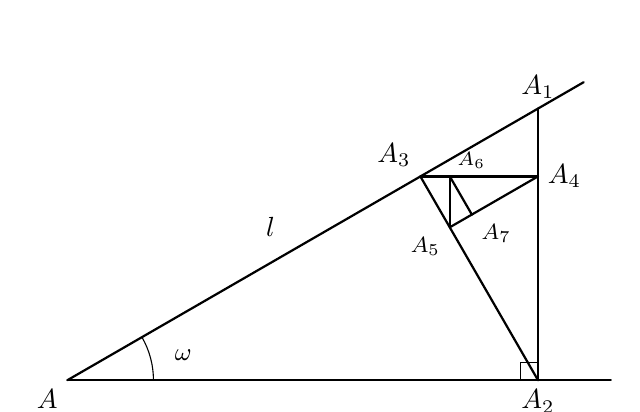
\begin{tikzpicture}[>=Stealth, scale=1.15, line cap=round, line join=round]
  % 兩直線交角 omega = 30 deg (exact perpendiculars matching original p.147)
  \coordinate (A) at (0, 0);
  \coordinate (X) at (6.0, 0);
  \coordinate (Y) at (5.7, 3.29);

  \draw[thick] (A) -- (X);
  \draw[thick] (A) -- (Y);
  \node[below left] at (A) {$A$};
  \draw[thin] (0.95, 0) arc (0:30:0.95);
  \node[font=\small] at (1.28, 0.28) {$\omega$};

  % 精確垂直足座標 (AA1 = 6, omega = 30 deg)
  \coordinate (A1) at (5.196, 3.000);
  \coordinate (A2) at (5.196, 0.000);
  \coordinate (A3) at (3.897, 2.250);
  \coordinate (A4) at (5.196, 2.250);
  \coordinate (A5) at (4.222, 1.688);
  \coordinate (A6) at (4.222, 2.250);
  \coordinate (A7) at (4.466, 1.828);

  \draw[thick] (A1) -- (A2);
  \draw[thick] (A2) -- (A3);
  \draw[thick] (A3) -- (A4);
  \draw[thick] (A4) -- (A5);
  \draw[thick] (A5) -- (A6);
  \draw[thick] (A6) -- (A7);

  \node[above] at (A1) {$A_1$};
  \node[below] at (A2) {$A_2$};
  \node[above left] at (A3) {$A_3$};
  \node[right] at (A4) {$A_4$};
  \node[below left, font=\footnotesize] at (A5) {$A_5$};
  \node[above right=-1pt, font=\scriptsize] at (A6) {$A_6$};
  \node[below right, font=\footnotesize] at (A7) {$A_7$};
  \node[above left] at (2.4, 1.48) {$l$};

  % 直角記號
  \draw[thin] (5.00, 0) -- (5.00, 0.20) -- (5.196, 0.20);
\end{tikzpicture}
\caption{無限交替垂線之幾何結構}
\label{fig:b6s-4-prob5}
\end{figure}

\paragraph{【解答】}
\begin{align*}
A_1 A_2 &= l \sin\omega \\
A_2 A_3 &= AA_2 \sin\omega = l \cos\omega \sin\omega \\
A_3 A_4 &= A_2 A_3 \sin\omega = l \cos\omega \sin^2\omega \\
A_4 A_5 &= A_3 A_4 \cos\omega = l \cos^2\omega \sin^2\omega \\
A_5 A_6 &= l \cos^2\omega \sin^3\omega \\
&\ \ \vdots
\end{align*}
即
\begin{align*}
S_1 &= l \sin\omega [1 + \cos\omega\sin\omega + (\cos\omega\sin\omega)^2 + (\cos\omega\sin\omega)^3 + \dots] \\
S_2 &= l \cos\omega\sin\omega [1 + \cos\omega\sin\omega + (\cos\omega\sin\omega)^2 + \dots]
\end{align*}
又因 $\omega$ 為銳角，$|\cos\omega\sin\omega| < 1$，故等比級數收斂，得：
\[ S_1 = \dfrac{l\sin\omega}{1-\cos\omega\sin\omega}, \quad S_2 = \dfrac{l\cos\omega\sin\omega}{1-\cos\omega\sin\omega} \]
即
\[ S = \dfrac{l\sin\omega(1+\cos\omega)}{1-\cos\omega\sin\omega} \text{。}\hfill\# \]

\paragraph{6. （39年度，臺大）}
設 $A+B+C=180^\circ$，試求下列行列式之值：
\[ \begin{vmatrix}
\sin^2 A & \cot A & 1 \\
\sin^2 B & \cot B & 1 \\
\sin^2 C & \cot C & 1
\end{vmatrix} \]

\paragraph{【分析】}
利用第二列減去第一列，第三列減去第一列，再利用三角形倍角與和角公式簡化。

\paragraph{【解答】}
\begin{align*}
\begin{vmatrix}
\sin^2 A & \cot A & 1 \\
\sin^2 B & \cot B & 1 \\
\sin^2 C & \cot C & 1
\end{vmatrix}
&= \begin{vmatrix}
\sin^2 A & \cot A & 1 \\
\sin^2 B - \sin^2 A & \cot B - \cot A & 0 \\
\sin^2 C - \sin^2 A & \cot C - \cot A & 0
\end{vmatrix} \\
&= \begin{vmatrix}
\frac{1}{2}(\cos 2A - \cos 2B) & \frac{\cos B}{\sin B} - \frac{\cos A}{\sin A} \\
\frac{1}{2}(\cos 2A - \cos 2C) & \frac{\cos C}{\sin C} - \frac{\cos A}{\sin A}
\end{vmatrix} \\
&= \begin{vmatrix}
\sin(B+A)\sin(B-A) & \frac{\sin(A-B)}{\sin A \sin B} \\
\sin(C+A)\sin(C-A) & \frac{\sin(A-C)}{\sin A \sin C}
\end{vmatrix} \\
&= \dfrac{\sin(A-B)\sin(A-C)}{\sin A \sin B \sin C} \begin{vmatrix}
-\sin(A+B) & \sin C \\
-\sin(A+C) & \sin B
\end{vmatrix} = 0
\end{align*}
因為 $\begin{cases} \sin(A+B) = \sin C \\ \sin(A+C) = \sin B \end{cases} \quad (A+B+C=180^\circ)$。\hfill$\#$

\paragraph{7.}
某學生每試五題平均可答出三題，今應試八題問至少能答出五題的或然率若干？

\paragraph{【分析】}
應先求出能答出八題、七題、六題、五題之或然率，再相加。（以上均為獨立事件）

\paragraph{【解答】}
此生答出一題之或然率為 $\dfrac{3}{5}$，不能答出一題之或然率為 $\dfrac{2}{5}$。
故能答出八題之或然率為 $\left(\dfrac{3}{5}\right)^8$，七題的為 ${}_8 C_7 \left(\dfrac{3}{5}\right)^7 \left(\dfrac{2}{5}\right)$，六題的為 ${}_8 C_6 \left(\dfrac{3}{5}\right)^6 \left(\dfrac{2}{5}\right)^2$，五題的為 ${}_8 C_5 \left(\dfrac{3}{5}\right)^5 \left(\dfrac{2}{5}\right)^3$。故得至少可答出五題的或然率為
\begin{align*}
&\left(\dfrac{3}{5}\right)^8 + {}_8 C_7 \left(\dfrac{3}{5}\right)^7 \left(\dfrac{2}{5}\right) + {}_8 C_6 \left(\dfrac{3}{5}\right)^6 \left(\dfrac{2}{5}\right)^2 + {}_8 C_5 \left(\dfrac{3}{5}\right)^5 \left(\dfrac{2}{5}\right)^3 \\
&= \dfrac{3^5}{5^8}(27 + 144 + 336 + 448) = \dfrac{46413}{78125} \text{。}\hfill\#
\end{align*}

\paragraph{8. （46年度，聯招）}
試解
\[ \begin{vmatrix}
1+x & 2 & 3 & 4 \\
1 & 2+x & 3 & 4 \\
1 & 2 & 3+x & 4 \\
1 & 2 & 3 & 4+x
\end{vmatrix} = 0 \]

\paragraph{【分析】}
顯然可看出各列的常數項均相同。

\paragraph{【解答】}
將第二、三、四行加前第一行，得
\begin{align*}
\begin{vmatrix}
1+x & 2 & 3 & 4 \\
1 & 2+x & 3 & 4 \\
1 & 2 & 3+x & 4 \\
1 & 2 & 3 & 4+x
\end{vmatrix}
&= \begin{vmatrix}
x+10 & 2 & 3 & 4 \\
x+10 & 2+x & 3 & 4 \\
x+10 & 2 & 3+x & 4 \\
x+10 & 2 & 3 & 4+x
\end{vmatrix} \\
&= (x+10) \begin{vmatrix}
1 & 2 & 3 & 4 \\
1 & 2+x & 3 & 4 \\
1 & 2 & 3+x & 4 \\
1 & 2 & 3 & 4+x
\end{vmatrix} \\
&= (x+10) \begin{vmatrix}
1 & 0 & 0 & 0 \\
1 & x & 0 & 0 \\
1 & 0 & x & 0 \\
1 & 0 & 0 & x
\end{vmatrix} = (x+10)x^3
\end{align*}
即 $(x+10)x^3 = 0$，得 $x = -10 \text{ 或 } 0$。\hfill$\#$

\paragraph{9. （50年度，聯招）}
\begin{enumerate}[label=(\alph*), leftmargin=2em]
  \item 利用絕對值之定義，方程式 $x+y=2$ 的圖形，及關於座標之對稱性，試作 $|x|+|y|=2$ 之圖。
  \item 應用 (a) 之結果試作 $|x-1|+|y-1|=2$ 之圖。
  \item 再應用 (b)，試作 $||x|-1| + ||y|-1| = 2$ 之圖。
\end{enumerate}

\paragraph{【分析】}
一個方程式 $f(x,y)=C$，若有 $f(x,y)=f(-x,y)$，表其圖形與 $y$ 軸對稱。若 $f(x,y)=f(x,-y)$，表其圖形與 $x$ 軸對稱。若 $f(x,y)=f(-x,-y)$ 表其圖形與原點對稱。若 $f(x,y)=f(y,x)$ 表其圖形與直線 $x=y$ 對稱。

\paragraph{【解答】}
\begin{enumerate}[label=(\alph*), leftmargin=2em]
  \item 因為 $|x|+|y| = |-x|+|y| = |x|+|-y| = |-x|+|-y|$。方程式 $|x|+|y|=2$ 之圖形應分別對稱於 $x$ 軸，$y$ 軸和原點，又知 $-2\le x\le 2, -2\le y\le 2$ 為必要條件。今在此範圍（第一象限）內 $x+y=2$ 的圖形如圖 1。故根據其對稱性繪出 $|x|+|y|=2$ 的圖形如圖 2（第 2, 3, 4 象限均含）。（注意：$CD$ 段亦可在畫出 $BC$ 段後根據對 $x$ 軸的對稱性而畫出）。
  \item 將座標平移到 $(1,1)$ 點，則可由 (a) 得到 $|x-1|+|y-1|=2$ 的圖形，見圖 3。
  \item 在 $x\ge 0, y\ge 0$，$||x|-1|+||y|-1|=2$ 之圖形恰當 (b) 之圖形相同。又可驗證此方程式對於 $x$ 軸、$y$ 軸、原點均對稱故可利用對稱性作圖 如圖 4。\hfill$\#$
\end{enumerate}

\begin{figure}[H]
\centering
\begin{subfigure}[b]{0.46\textwidth}
\centering
\begin{tikzpicture}[>=Stealth, scale=0.72, line cap=round]
  \draw[->] (-0.8, 0) -- (3.2, 0) node[right] {\footnotesize $X$};
  \draw[->] (0, -0.8) -- (0, 3.2) node[above] {\footnotesize $Y$};
  \draw[thick] (2, 0) -- (0, 2);
  \node[above right] at (2, 0) {\footnotesize $A$};
  \node[below] at (2, 0) {\footnotesize $2$};
  \node[above right] at (0, 2) {\footnotesize $B$};
  \node[left] at (0, 2) {\footnotesize $2$};
\end{tikzpicture}
\caption{圖 1}
\end{subfigure}
\hfill
\begin{subfigure}[b]{0.46\textwidth}
\centering
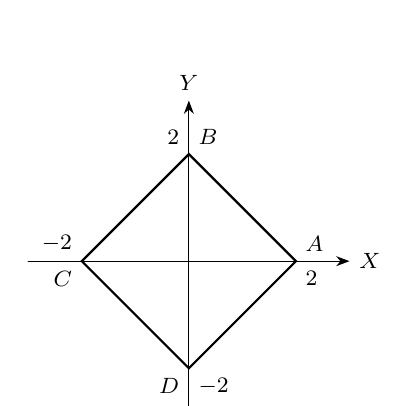
\begin{tikzpicture}[>=Stealth, scale=0.68, line cap=round]
  \draw[->] (-3.0, 0) -- (3.0, 0) node[right] {\footnotesize $X$};
  \draw[->] (0, -2.9) -- (0, 3.0) node[above] {\footnotesize $Y$};
  \draw[thick] (2, 0) -- (0, 2) -- (-2, 0) -- (0, -2) -- cycle;
  \node[above right] at (0, 2) {\footnotesize $B$};
  \node[above left] at (0, 2) {\footnotesize $2$};
  \node[above right] at (2, 0) {\footnotesize $A$};
  \node[below right] at (2, 0) {\footnotesize $2$};
  \node[above left] at (-2, 0) {\footnotesize $-2$};
  \node[below left] at (-2, 0) {\footnotesize $C$};
  \node[below left] at (0, -2) {\footnotesize $D$};
  \node[below right] at (0, -2) {\footnotesize $-2$};
\end{tikzpicture}
\caption{圖 2}
\end{subfigure}

\vspace{0.8em}
\begin{subfigure}[b]{0.46\textwidth}
\centering
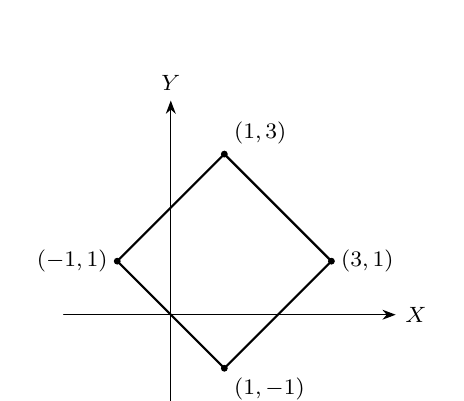
\begin{tikzpicture}[>=Stealth, scale=0.68, line cap=round]
  \draw[->] (-2.0, 0) -- (4.2, 0) node[right] {\footnotesize $X$};
  \draw[->] (0, -1.8) -- (0, 4.0) node[above] {\footnotesize $Y$};
  \draw[thick] (3, 1) -- (1, 3) -- (-1, 1) -- (1, -1) -- cycle;
  \filldraw (1, 3) circle (1.5pt) node[above right] {\footnotesize $(1,3)$};
  \filldraw (3, 1) circle (1.5pt) node[right] {\footnotesize $(3,1)$};
  \filldraw (-1, 1) circle (1.5pt) node[left] {\footnotesize $(-1,1)$};
  \filldraw (1, -1) circle (1.5pt) node[below right] {\footnotesize $(1,-1)$};
\end{tikzpicture}
\caption{圖 3}
\end{subfigure}
\hfill
\begin{subfigure}[b]{0.46\textwidth}
\centering
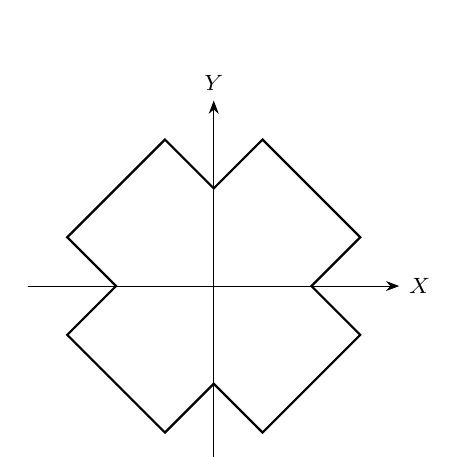
\begin{tikzpicture}[>=Stealth, scale=0.62, line cap=round]
  \draw[->] (-3.8, 0) -- (3.8, 0) node[right] {\footnotesize $X$};
  \draw[->] (0, -3.7) -- (0, 3.8) node[above] {\footnotesize $Y$};
  % 四個象限對稱拼接圖形
  \draw[thick] (3, 1) -- (1, 3) -- (0, 2) -- (-1, 3) -- (-3, 1) -- (-2, 0) -- (-3, -1) -- (-1, -3) -- (0, -2) -- (1, -3) -- (3, -1) -- (2, 0) -- cycle;
\end{tikzpicture}
\caption{圖 4}
\end{subfigure}
\caption{含絕對值之線性幾何對稱圖形}
\label{fig:b6s-4-prob9}
\end{figure}

\paragraph{10. （51年度，聯招）}
解下列不等式
\[ \begin{vmatrix}
1-x & 4 & 1 & 1 \\
1 & 2-x & 3 & 1 \\
1 & 1 & 3-x & 2 \\
1 & 1 & 1 & 4-x
\end{vmatrix} > 0 \]

\paragraph{【分析】}
同第八題，各列係數和相等，各行加到第一行。

\paragraph{【解答】}
\begin{align*}
\begin{vmatrix}
1-x & 4 & 1 & 1 \\
1 & 2-x & 3 & 1 \\
1 & 1 & 3-x & 2 \\
1 & 1 & 1 & 4-x
\end{vmatrix}
&= \begin{vmatrix}
7-x & 4 & 1 & 1 \\
7-x & 2-x & 3 & 1 \\
7-x & 1 & 3-x & 2 \\
7-x & 1 & 1 & 4-x
\end{vmatrix} \\
&= (7-x) \begin{vmatrix}
1 & 4 & 1 & 1 \\
1 & 2-x & 3 & 1 \\
1 & 1 & 3-x & 2 \\
1 & 1 & 1 & 4-x
\end{vmatrix} \\
&= (7-x) \begin{vmatrix}
1 & 4 & 1 & 1 \\
0 & -2-x & 2 & 0 \\
0 & -3 & 2-x & 1 \\
0 & -3 & 0 & 3-x
\end{vmatrix} \\
&= (7-x) \begin{vmatrix}
-2-x & 2 & 0 \\
-3 & 2-x & 1 \\
-3 & 0 & 3-x
\end{vmatrix} \\
&= (7-x) \begin{vmatrix}
-x & 2 & 0 \\
-x & 2-x & 1 \\
-x & 0 & 3-x
\end{vmatrix} \\
&= x(x-7) \begin{vmatrix}
1 & 2 & 0 \\
1 & 2-x & 1 \\
1 & 0 & 3-x
\end{vmatrix} = x(x-7) \begin{vmatrix}
1 & 2 & 0 \\
0 & -x & 1 \\
0 & -2 & 3-x
\end{vmatrix} \\
&= x(x-7) \begin{vmatrix}
-x & 1 \\
-2 & 3-x
\end{vmatrix} = x(x-7)(x-2)(x-1)
\end{align*}
故得 $x(x-1)(x-2)(x-7) > 0$。

今由下表：
\begin{center}
\renewcommand{\arraystretch}{1.2}
\begin{tabular}{c|c|c|c|c|c}
& $x<0$ & $0<x<1$ & $1<x<2$ & $2<x<7$ & $7<x$ \\ \hline
$x$ & $-$ & $+$ & $+$ & $+$ & $+$ \\
$x-1$ & $-$ & $-$ & $+$ & $+$ & $+$ \\
$x-2$ & $-$ & $-$ & $-$ & $+$ & $+$ \\
$x-7$ & $-$ & $-$ & $-$ & $-$ & $+$ \\ \hline
$f(x)$ & $+$ & $-$ & $+$ & $-$ & $+$
\end{tabular}
\end{center}
故得 $x<0$ 或 $1<x<2$ 或 $7<x$。\hfill$\#$

\paragraph{註：} 另有一簡便之法如下，從 7 的右邊起畫正、負號相間：
\begin{center}
\begin{tikzpicture}[scale=1.0]
  \draw[thick, ->] (-1, 0) -- (8.5, 0);
  \foreach \x in {0, 1, 2, 7} {
    \draw (\x, 0.1) -- (\x, -0.1) node[below] {$\x$};
  }
  \node[above] at (-0.5, 0.1) {$+$};
  \node[above] at (0.5, 0.1) {$-$};
  \node[above] at (1.5, 0.1) {$+$};
  \node[above] at (4.5, 0.1) {$-$};
  \node[above] at (7.8, 0.1) {$+$};
\end{tikzpicture}
\end{center}
故取 $7<x$ 或 $1<x<2$ 或 $x<0$。

\paragraph{11. （52年度，聯招）}
設正三角形 $ABC$ 之一邊長為 $k$；今依 $AB, BC, CA$ 之順序將其各區分為 $1:2$ 之點命為 $A_1, B_1, C_1$；其次依 $A_1 B_1, B_1 C_1, C_1 A_1$ 之順序，將三角形 $A_1 B_1 C_1$ 之各邊分為 $1:2$ 之邊命為 $A_2, B_2, C_2$；再次同樣，如此繼續無窮次，試求 $ABC, A_1 B_1 C_1, A_2 B_2 C_2, \dots$ 等無限個三角形面積之總和。

\paragraph{【分析】}
我們猜測各三角形均相似，且其面積比成一等比級數。

\paragraph{【解答】}
首先，$\angle A_1 B B_1 = \dfrac{\pi}{3}, \quad \overline{A_1 B} = 2\overline{BB_1}$，故 $\angle A_1 B_1 B = \dfrac{\pi}{2}$。所以
\[ A_1 B_1 = A_1 B \sin\dfrac{\pi}{3} = \dfrac{2}{3}k \cdot \dfrac{\sqrt{3}}{2} = \dfrac{\sqrt{3}}{3}k \]
故得知 $\triangle A_1 B_1 C_1$ 亦為正三角形，同理 $\triangle A_n B_n C_n$ 均為正三角形，故均相似。

\begin{figure}[H]
\centering
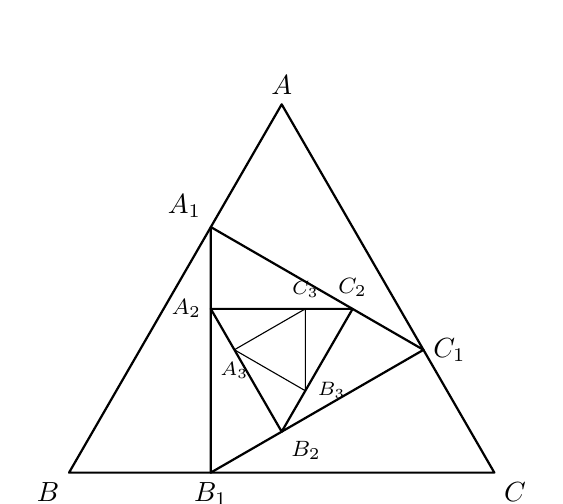
\begin{tikzpicture}[>=Stealth, scale=1.35, line cap=round, line join=round]
  \coordinate (A) at (0, 3.464);
  \coordinate (B) at (-2, 0);
  \coordinate (C) at (2, 0);

  \draw[thick] (A) -- (B) -- (C) -- cycle;
  \node[above] at (A) {$A$};
  \node[below left] at (B) {$B$};
  \node[below right] at (C) {$C$};

  % 依 AB, BC, CA 順序作 1:2 分點 (AA1:A1B = 1:2, 使 A1B1 垂直於 BC, 與原書 p.154 一致)
  \coordinate (A1) at ($(A)!0.3333!(B)$);
  \coordinate (B1) at ($(B)!0.3333!(C)$);
  \coordinate (C1) at ($(C)!0.3333!(A)$);

  \draw[thick] (A1) -- (B1) -- (C1) -- cycle;
  \node[above left] at (A1) {$A_1$};
  \node[below] at (B1) {$B_1$};
  \node[right] at (C1) {$C_1$};

  % 第二層 1:2 分點
  \coordinate (A2) at ($(A1)!0.3333!(B1)$);
  \coordinate (B2) at ($(B1)!0.3333!(C1)$);
  \coordinate (C2) at ($(C1)!0.3333!(A1)$);

  \draw[thick] (A2) -- (B2) -- (C2) -- cycle;
  \node[left, font=\footnotesize] at (A2) {$A_2$};
  \node[below right, font=\footnotesize] at (B2) {$B_2$};
  \node[above=1pt, font=\footnotesize] at (C2) {$C_2$};

  % 第三層 1:2 分點
  \coordinate (A3) at ($(A2)!0.3333!(B2)$);
  \coordinate (B3) at ($(B2)!0.3333!(C2)$);
  \coordinate (C3) at ($(C2)!0.3333!(A2)$);

  \draw[thin] (A3) -- (B3) -- (C3) -- cycle;
  \node[below=1pt, font=\scriptsize] at (A3) {$A_3$};
  \node[right=1pt, font=\scriptsize] at (B3) {$B_3$};
  \node[above=0.5pt, font=\scriptsize] at (C3) {$C_3$};
\end{tikzpicture}
\caption{無限正三角形縮小嵌套結構}
\label{fig:b6s-4-prob11}
\end{figure}

所以，
\[ \dfrac{\triangle A_1 B_1 C_1 \text{ 面積}}{\triangle ABC \text{ 面積}} = \dfrac{A_1 B_1^2}{AB^2} = \dfrac{(\frac{\sqrt{3}}{3}k)^2}{k^2} = \dfrac{1}{3} \]
即
\[ \triangle A_n B_n C_n \text{ 面積} = \dfrac{1}{3}\triangle A_{n-1} B_{n-1} C_{n-1} \text{ 面積} = \dfrac{1}{3^n}\triangle ABC \text{ 面積} \]
今 $\triangle ABC \text{ 面積} = \dfrac{\sqrt{3}}{4}k^2$
\begin{align*}
\therefore S &= \triangle ABC \text{ 面積} + \triangle A_1 B_1 C_1 \text{ 面積} + \triangle A_2 B_2 C_2 \text{ 面積} + \dots \\
&= \dfrac{\sqrt{3}}{4}k^2 \left(1 + \dfrac{1}{3} + \dfrac{1}{3^2} + \dfrac{1}{3^3} + \dots\right) = \dfrac{\sqrt{3}}{4}k^2 \cdot \dfrac{1}{1-\frac{1}{3}} = \dfrac{3\sqrt{3}}{8}k^2 \text{。}\hfill\#
\end{align*}

\paragraph{12. （53年度，聯招）}
設 $a_1, a_2, \dots, a_n; b_1, b_2, \dots, b_n$ 及 $k$ 均為實數，求下列等式中之 $p, q, r$：
\[ (ka_1+b_1)^2 + (ka_2+b_2)^2 + \dots + (ka_n+b_n)^2 = pk^2 + 2qk + r \]
並由此推出不等式
\[ (a_1 b_1 + a_2 b_2 + \dots + a_n b_n)^2 \le (a_1^2 + a_2^2 + \dots + a_n^2)(b_1^2 + b_2^2 + \dots + b_n^2) \]

\paragraph{【分析】}
顯然須利用判別式 $\ge 0$ 的性質。

\paragraph{【解答】}
由前式左邊，顯然得 $pk^2+2qk+r \ge 0$，又
\begin{align*}
p &= (a_1^2+a_2^2+\dots+a_n^2) \\
q &= (a_1 b_1 + a_2 b_2 + \dots + a_n b_n) \\
r &= (b_1^2+b_2^2+\dots+b_n^2)
\end{align*}
今 $p\ge 0$，無論 $k$ 值為何恆有 $pk^2+2qk+r \ge 0$ 的充要條件為 $q^2-pr \le 0$，即
\[ (a_1 b_1 + a_2 b_2 + \dots + a_n b_n)^2 \le (a_1^2+a_2^2+\dots+a_n^2)(b_1^2+b_2^2+\dots+b_n^2) \text{。}\hfill\# \]

\paragraph{13. （54年度，聯招）}
設 $n$ 為正整數
\begin{enumerate}[label=(\alph*), leftmargin=2em]
  \item 解方程式 $x^n-1=0$（求複數解）
  \item 證明：
  \begin{align*}
  1 + \cos\dfrac{2\pi}{n} + \cos\dfrac{4\pi}{n} + \dots + \cos\dfrac{2(n-1)\pi}{n} &= 0 \\
  \sin\dfrac{2\pi}{n} + \sin\dfrac{4\pi}{n} + \dots + \sin\dfrac{2(n-1)\pi}{n} &= 0
  \end{align*}
\end{enumerate}

\paragraph{【分析】}
\begin{enumerate}[label=(\alph*), leftmargin=2em]
  \item 顯然需用 DeMoivre 定理。
  \item 在解決 (a) 解以後，很自然想到利用根與係數關係。因在 $x^n-1=0$ 中，諸根之和為 0，又若 $a+bi=0$ 則 $a=b=0$。
\end{enumerate}

\paragraph{【解答】}
\begin{enumerate}[label=(\alph*), leftmargin=2em]
  \item $x^n = 1 = \cos 2k\pi + i\sin 2k\pi$，即
  \[ x_k = \cos\dfrac{2k\pi}{n} + i\sin\dfrac{2k\pi}{n}, \quad k=0, 1, 2, \dots, n-1 \text{ 得所求 } n \text{ 個根。} \]
  \item 因（諸根之和）$= -(x^{n-1} \text{ 的係數}) = 0$，得
  \begin{align*}
  &1 + \left(\cos\dfrac{2\pi}{n}+i\sin\dfrac{2\pi}{n}\right) + \left(\cos\dfrac{4\pi}{n}+i\sin\dfrac{4\pi}{n}\right) + \dots \\
  &\quad + \left(\cos\dfrac{2(n-1)\pi}{n}+i\sin\dfrac{2(n-1)\pi}{n}\right) = 0
  \end{align*}
  得實部與虛部分別為 0：
  \begin{align*}
  1 + \cos\dfrac{2\pi}{n} + \cos\dfrac{4\pi}{n} + \dots + \cos\dfrac{2(n-1)\pi}{n} &= 0 \\
  \sin\dfrac{2\pi}{n} + \sin\dfrac{4\pi}{n} + \dots + \sin\dfrac{2(n-1)\pi}{n} &= 0 \text{。}\hfill\#
  \end{align*}
\end{enumerate}

\paragraph{注意：} (b) 亦可由三角級數法求和。提示：令 $\alpha=\dfrac{2\pi}{n}$，則 $\sin\dfrac{\alpha}{2} = \sin\dfrac{\pi}{n}\ne 0$，考慮 $\cos\dfrac{2k\pi}{n} = \dfrac{1}{2\sin\frac{\alpha}{2}}\left(2\cos k\alpha \sin\dfrac{\alpha}{2}\right)$ 利用積化和。對 $\sin\dfrac{2k\pi}{n}$ 亦同樣做。

\paragraph{14. （54年度，聯招）}
設 $a, b$ 皆為實數，$ab\ne 0$，證明 $ax^2+2bxy-ay^2=0$ 之圖形為二直線互相垂直。

\paragraph{【分析】}
此二直線均過原點，故可分別表為 $y-m_1 x = 0$ 及 $y-m_2 x = 0$，只須驗證 $m_1 m_2 = -1$。

\paragraph{【解答】}
原式可寫為 $y^2 - 2\dfrac{b}{a}xy - x^2 = 0$。今
\[ (y-m_1 x)(y-m_2 x) = y^2 - (m_1+m_2)xy + m_1 m_2 x^2 = y^2 - 2\dfrac{b}{a}xy - x^2 \]
對應係數，得 $m_1 m_2 = -1$。\hfill$\#$

\paragraph{注意：} 亦可將 $y^2-2\dfrac{b}{a}xy-x^2$ 分解因式，解出 $m_1, m_2$，再驗證 $m_1 m_2 = -1$，但較繁複多矣。

\paragraph{15.}
已知一函數 $f(x)$ 具有下列諸性質：
\[ f(x+5) = f(x), \quad f(-x) = -f(x), \quad f\left(\dfrac{1}{3}\right) = 1 \]
試求
\begin{enumerate}[label=(\alph*), leftmargin=2em]
  \item $f\left(\dfrac{16}{3}\right)$
  \item $f\left(\dfrac{29}{3}\right)$
  \item $f(12)+f(-7)$
\end{enumerate}

\paragraph{【分析】}
這不一定是一個多項式（其實根本不是）。我們注意到 $\dfrac{16}{3} = 5+\dfrac{1}{3}, \dfrac{29}{3} = 10-\dfrac{1}{3}$。

\paragraph{【解答】}
\begin{enumerate}[label=(\alph*), leftmargin=2em]
  \item $f\left(\dfrac{16}{3}\right) = f\left(5+\dfrac{1}{3}\right) = f\left(\dfrac{1}{3}\right) = 1$
  \item $f\left(\dfrac{29}{3}\right) = f\left(5+\left(5-\dfrac{1}{3}\right)\right) = f\left(5-\dfrac{1}{3}\right) = f\left(-\dfrac{1}{3}\right) = -f\left(\dfrac{1}{3}\right) = -1$
  \item $f(12)+f(-7) = f(10+2)-f(7) = f(2)-f(2) = 0$。\hfill$\#$
\end{enumerate}

\paragraph{16. （55年度，聯招）}
設 $z = x+iy$，其中 $x, y$ 均為實數而 $i^2 = -1$。證明
\[ |z| \le |x|+|y| \le \sqrt{2}|z| \]

\paragraph{【分析】}
左邊不等式，從向量的觀點為顯然。右邊不等式可以直接去計算。

\paragraph{【解答】}
\begin{enumerate}[label=(\alph*), leftmargin=2em]
  \item $|z| = \sqrt{x^2+y^2}$。利用三角形兩邊和大於第三邊的關係，得 $|z| \le |x|+|y|$。
  \item $(|x|+|y|)^2 - (\sqrt{2}|z|)^2 = x^2+2|x||y|+y^2 - 2(x^2+y^2) = -(x^2-2|x||y|+y^2) = -(|x|-|y|)^2 \le 0$，即 $|x|+|y| \le \sqrt{2}|z|$。\hfill$\#$
\end{enumerate}

\begin{figure}[H]
\centering
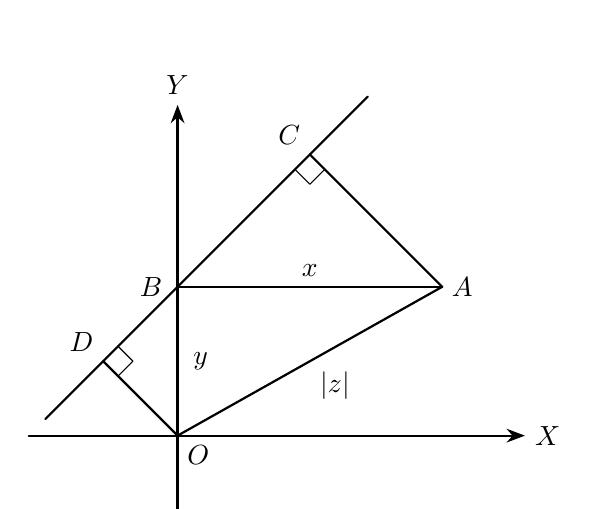
\begin{tikzpicture}[>=Stealth, scale=1.05, line cap=round, line join=round]
  \coordinate (O) at (0, 0);
  \coordinate (X) at (4.2, 0);
  \coordinate (Y) at (0, 4.0);

  \draw[->, thick] (-1.8, 0) -- (X) node[right] {$X$};
  \draw[->, thick] (0, -1.0) -- (Y) node[above] {$Y$};
  \node[below right] at (O) {$O$};

  % 點 A(x, y), B(0, y)
  \coordinate (A) at (3.2, 1.8);
  \coordinate (B) at (0, 1.8);

  \draw[thick] (O) -- (A) node[midway, below right] {$|z|$};
  \draw[thick] (B) -- (A) node[midway, above] {$x$};
  \draw[thick] (O) -- (B) node[midway, right=2pt] {$y$};
  \node[right] at (A) {$A$};
  \node[left=2pt] at (B) {$B$};

  % 過 B 斜率為 1 之直線 y = x + 1.8，以及 A, O 之正交投影 C(1.6, 3.4), D(-0.9, 0.9)
  \draw[thick] (-1.6, 0.2) -- (2.3, 4.1);
  \coordinate (C) at (1.6, 3.4);
  \coordinate (D) at (-0.9, 0.9);

  \draw[thick] (A) -- (C);
  \draw[thick] (O) -- (D);

  % 直角記號於 C 與 D
  \draw[thin] ($(C)+(-0.18,-0.18)$) -- ($(C)+(0,-0.36)$) -- ($(C)+(0.18,-0.18)$);
  \draw[thin] ($(D)+(0.18,0.18)$) -- ($(D)+(0.36,0)$) -- ($(D)+(0.18,-0.18)$);

  \node[above left] at (C) {$C$};
  \node[above left] at (D) {$D$};
\end{tikzpicture}
\caption{$|z| \le |x|+|y| \le \sqrt{2}|z|$ 之幾何投影證明}
\label{fig:b6s-4-prob16}
\end{figure}

\paragraph{注意：} (b) 亦可由幾何得到解決（考慮第一象限）：自 $B$ 作斜率為 1 的直線，則
\[ \overline{BC} = \overline{AB}\cos\dfrac{\pi}{4} = \dfrac{x}{\sqrt{2}}, \quad \overline{BD} = \overline{OB}\cos\dfrac{\pi}{4} = \dfrac{y}{\sqrt{2}} \]
今由於 $\angle ACB, \angle BDO$ 均為直角，
\[ \overline{OA} \ge \overline{CD} = \overline{BC}+\overline{BD} = \dfrac{x}{\sqrt{2}} + \dfrac{y}{\sqrt{2}} \]
即 $|z| \ge \dfrac{1}{\sqrt{2}}(|x|+|y|)$，或 $|x|+|y| \le \sqrt{2}|z|$。

\paragraph{17. （56年度，聯招）}
方程式 $\sqrt{x} - \sqrt{x+\sqrt{x-1}} = 1$ 有幾個實根？
\begin{multicols}{2}
\begin{enumerate}[label=(\Alph*)]
  \item 一個
  \item 兩個
  \item 三個
  \item 四個
  \item 以上皆非
\end{enumerate}
\end{multicols}

\paragraph{【分析】}
用最簡方式將之先有理化。

\paragraph{【解答】}
$\sqrt{x}-1 = \sqrt{x+\sqrt{x-1}}$，兩邊平方：
\[ x - 2\sqrt{x} + 1 = x + \sqrt{x-1} \implies 1-2\sqrt{x} = \sqrt{x-1} \]
再平方：
\[ 1-4\sqrt{x}+4x = x-1 \implies 2+3x = 4\sqrt{x} \]
再平方：
\[ 4+12x+9x^2 = 16x \implies 9x^2-4x+4 = 0 \]
判別式 $= 16 - 144 < 0$，無實根，故答案為 (E)。\hfill$\#$

\paragraph{注意：} 這種有開根號的方程式，就是有根也需代入原式驗證，因在平方時很可能引進一些新的或不合理的根。

\paragraph{18. （56年度，聯招）}
方程式
\[ \begin{vmatrix}
a_{11}-x & a_{12} & \dots & a_{1n} \\
a_{21} & a_{22}-x & \dots & a_{2n} \\
\vdots & \vdots & \ddots & \vdots \\
a_{n1} & a_{n2} & \dots & a_{nn}-x
\end{vmatrix} = 0 \]
諸根的乘積是：
\begin{multicols}{2}
\begin{enumerate}[label=(\Alph*)]
  \item $a_{11}+a_{22}+\dots+a_{nn}$
  \item $(-1)^n (a_{11}+a_{22}+\dots+a_{nn})$
  \item $|a_{ij}|_n$
  \item $(-1)^n |a_{ij}|_n$
  \item 以上皆非
\end{enumerate}
\end{multicols}

\paragraph{【分析】}
這是行列式與方程式論的混合題。我們知道一個多項式 $f(x)$ 的常數項為 $f(0)$。又一 $n$ 次多項式之 $n$ 次項係數除其常數項所得商之 $(-1)^n$ 為諸根之乘積。

\paragraph{【解答】}
設
\[ f(x) = \begin{vmatrix}
a_{11}-x & a_{12} & \dots & a_{1n} \\
a_{21} & a_{22}-x & \dots & a_{2n} \\
\vdots & \vdots & \ddots & \vdots \\
a_{n1} & a_{n2} & \dots & a_{nn}-x
\end{vmatrix} \]
則 $f(x)$ 為一 $n$ 次多項式，其 $n$ 次項係數為 $(-1)^n$，常數項 $f(0) = |a_{ij}|_n$。故諸根乘積 $= (-1)^n \dfrac{|a_{ij}|_n}{(-1)^n} = |a_{ij}|_n$。答案為 (C)。\hfill$\#$

\paragraph{19. （57年度，聯招）}
兩觀測站 $S_1, S_2$ 之距離為 $r$；飛機 $A$ 在地面 $B$ 點上空。$S_1$ 站測得 $A$ 之仰角為 $\phi$。$\angle BS_1 S_2 = \psi$；$S_2$ 站測得 $\angle BS_2 S_1 = \theta$，則飛機高 $\overline{AB}$ 為：
\begin{multicols}{2}
\begin{enumerate}[label=\tiangan*]
  \item $r\dfrac{\sin\theta\sin\phi}{\sin(\theta+\psi)}$
  \item $r\dfrac{\sin\theta\tan\phi}{\sin(\theta+\psi)}$
  \item $r\dfrac{\cot\phi\cot\psi+\sqrt{\cot^2\phi\csc^2\psi-\cot^2\theta}}{\cot^2\theta-\cot^2\psi}$
  \item $r\dfrac{\cot\phi\cot\psi-\sqrt{\cot^2\phi\csc^2\psi-\cot^2\theta}}{\cot^2\theta-\cot^2\psi}$
  \item 以上皆非
\end{enumerate}
\end{multicols}

\begin{figure}[H]
\centering
\begin{tikzpicture}[>=Stealth, scale=1.05, line cap=round, line join=round]
  \coordinate (S1) at (0, 0);
  \coordinate (S2) at (4.8, 0);
  \coordinate (B) at (3.2, 1.7);
  \coordinate (A) at (3.2, 4.1);

  \draw[thick] (S1) -- (S2) node[midway, below] {$r$};
  \draw[thick] (S1) -- (B);
  \draw[thick] (S2) -- (B);
  \draw[line width=1.4pt] (B) -- (A) node[midway, left=3pt] {高};
  \draw[thick] (S1) -- (A);
  \draw[dashed] (S2) -- (A);

  % 直角記號於 B (AB 垂直地面 S1B)
  \draw[thin] (3.2, 1.98) -- (2.96, 1.85) -- (2.96, 1.57);

  \node[below left] at (S1) {$S_1$};
  \node[below right] at (S2) {$S_2$};
  \node[above] at (A) {$A$};
  \node[right=2pt] at (B) {$B$};

  \draw[thin] (0.95, 0) arc (0:28:0.95);
  \node[font=\small] at (1.22, 0.25) {$\psi$};
  \draw[thin] (0.72, 0.38) arc (28:52:0.82);
  \node[font=\small] at (0.85, 0.72) {$\phi$};
  \draw[thin] (4.15, 0) arc (180:133:0.65);
  \node[font=\small] at (4.05, 0.28) {$\theta$};
\end{tikzpicture}
\caption{飛機高度之立體三角觀測模型}
\label{fig:b6s-4-prob19}
\end{figure}

\paragraph{【解答】}
$\overline{AB} = \overline{S_1 B}\tan\phi$。又在 $\triangle S_1 B S_2$ 中，由正弦定理：
\[ \dfrac{\sin\theta}{\overline{S_1 B}} = \dfrac{\sin(\pi-(\psi+\theta))}{r} \implies \overline{S_1 B} = \dfrac{r\sin\theta}{\sin(\psi+\theta)} \]
故
\[ \overline{AB} = \overline{S_1 B}\tan\phi = \dfrac{r\sin\theta\tan\phi}{\sin(\psi+\theta)} \]
故答案為 (乙)。\hfill$\#$

\paragraph{20. （57年度，聯招）}
方程式 $x^2+4xy+4y^2-2x-4y-3=0$ 的圖形是：
\begin{multicols}{2}
\begin{enumerate}[label=\tiangan*]
  \item 橢圓
  \item 雙曲線
  \item 兩平行直線之聯集
  \item 兩相交直線之聯集
  \item 以上皆非
\end{enumerate}
\end{multicols}

\paragraph{【解答】}
$B^2-AC = 4-4=0$ 為直線，因式分解：
\begin{align*}
x^2+(4y-2)x+(4y^2-4y-3) &= 0 \\
x^2+2(2y-1)x+(2y+1)(2y-3) &= 0 \\
(x+2y+1)(x+2y-3) &= 0
\end{align*}
所得二直線 $x+2y+1=0, x+2y-3=0$ 為平行。答案為 (丙)。\hfill$\#$

\paragraph{21. （57年度，聯招）}
令 $O$ 為 $\triangle ABC$ 內部之一點，設射線 $\vec{AO}$ 交 $\overline{BC}$ 於 $D$，$\vec{BO}$ 交 $\overline{CA}$ 於 $E$，$\vec{CO}$ 交 $\overline{AB}$ 於 $F$。令 $P = AB+BC+CA, q = AD+BE+CF$。則必有：
\begin{multicols}{2}
\begin{enumerate}[label=\tiangan*]
  \item $q < \frac{1}{3}P$
  \item $\frac{1}{3}P \le q \le \frac{1}{2}P$
  \item $\frac{1}{2}P < q < \frac{3}{2}P$
  \item $\frac{3}{2}P \le q \le 2P$
  \item 以上皆非
\end{enumerate}
\end{multicols}

\begin{figure}[H]
\centering
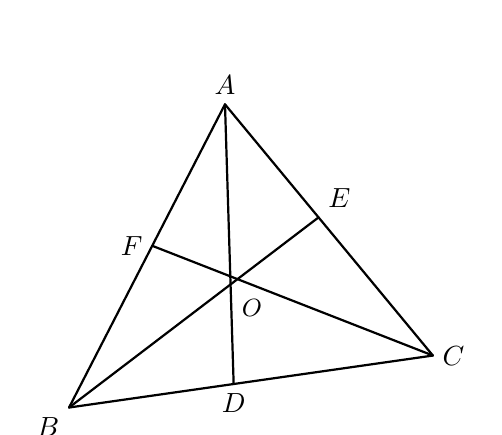
\begin{tikzpicture}[>=Stealth, scale=1.1, line cap=round, line join=round]
  \coordinate (A) at (1.8, 3.5);
  \coordinate (B) at (0, 0);
  \coordinate (C) at (4.2, 0.6);

  % 重心內部點 O 及三條準確共點塞瓦線
  \coordinate (D) at (1.9, 0.271);
  \coordinate (E) at (2.88, 2.195);
  \coordinate (F) at (0.96, 1.867);
  \coordinate (O) at (1.84, 1.40);

  \draw[thick] (A) -- (B) -- (C) -- cycle;
  \draw[thick] (A) -- (D);
  \draw[thick] (B) -- (E);
  \draw[thick] (C) -- (F);

  \node[above] at (A) {$A$};
  \node[below left] at (B) {$B$};
  \node[right] at (C) {$C$};
  \node[below] at (D) {$D$};
  \node[above right] at (E) {$E$};
  \node[left] at (F) {$F$};
  \node[below right=1pt, font=\small] at (1.86, 1.38) {$O$};
\end{tikzpicture}
\caption{三角形內部線段之不等式關係}
\label{fig:b6s-4-prob21}
\end{figure}

\paragraph{【解答】}
在 $\triangle ABD$ 中，$AB < AD+BD$；於 $\triangle ACD$ 中，$AC < AD+CD$。兩邊相加：
\[ AB+AC < 2AD+BC \implies AB+AC-BC < 2AD \]
同理 $AB+BC-AC < 2BE, AC+BC-AB < 2CF$。三式相加得：
\[ \dfrac{1}{2}(AB+BC+CA) < AD+BE+CF \tag{1} \]
又在 $\triangle ABD$ 中，$AD < AB+BD$；於 $\triangle ACD$ 中，$AD < AC+CD$。邊邊相加得 $2AD < AB+AC+BC$。同理可得
\[ AD+BE+CF < \dfrac{3}{2}(AB+BC+AC) \tag{2} \]
綜合 (1), (2) 得 $\dfrac{1}{2}P < q < \dfrac{3}{2}P$。答案：丙。\hfill$\#$

\paragraph{22. （57年度，聯招）}
方程式 $\log_6 x + \log_6(x^2-7) = 1$ 的解集合之元素個數為：
\begin{multicols}{2}
\begin{enumerate}[label=\tiangan*]
  \item 0
  \item 1
  \item 2
  \item 3
  \item 以上皆非
\end{enumerate}
\end{multicols}

\paragraph{【解答】}
由原式得 $\log_6 x(x^2-7) = 1 \implies x(x^2-7) = 6 \implies x^3-7x-6 = 0$。
分解得 $(x+1)(x+2)(x-3) = 0$。
因需 $x>0, x^2-7>0$，故只能取 $x=3$。元素個數為 1。答案：(乙)（原書誤寫為丁，實為 1 個解，即乙）。\hfill$\#$

\paragraph{23. （58年度，聯招）}
設 $a, b$ 為實數，若已知方程式 $x^3+ax+b=0$ 之一複數根為 $1+i$，則 $\dfrac{a}{b}$ 滿足下列不等式：
\begin{multicols}{2}
\begin{enumerate}[label=\tiangan*]
  \item $-1 \le \frac{a}{b} < -\frac{2}{3}$
  \item $-\frac{2}{3} \le \frac{a}{b} < -\frac{1}{3}$
  \item $-\frac{1}{3} \le \frac{a}{b} < 0$
  \item $0 \le \frac{a}{b} < \frac{1}{3}$
  \item $\frac{1}{3} \le \frac{a}{b} < \frac{2}{3}$
  \item $\frac{2}{3} \le \frac{a}{b} < 1$
  \item $1 \le \frac{a}{b} < \frac{4}{3}$
  \item $\frac{4}{3} \le \frac{a}{b} < \frac{5}{3}$
\end{enumerate}
\end{multicols}

\paragraph{【解答】}
實係數方程式有根 $1+i$，必有共軛根 $1-i$。故
\[ x^3+ax+b \text{ 能為 } (x-1-i)(x-1+i) = x^2-2x+2 \text{ 所整除。} \]
令 $x^3+ax+b = (x^2-2x+2)(x-\alpha) = x^3 - (\alpha+2)x^2 + (2+2\alpha)x - 2\alpha$。
得 $\alpha = -2, a = 2+2\alpha = -2, b = 4$。
故 $\dfrac{a}{b} = -\dfrac{1}{2}$。答案：(乙)。\hfill$\#$

\paragraph{24. （58年度，聯招）}
$xyz$ 一平面之一點 $(1, 0, -1)$ 及一直線 $\dfrac{x-1}{4} = \dfrac{y-2}{5} = \dfrac{z-3}{6}$ 決定一平面，其平面方程式為：
\begin{multicols}{2}
\begin{enumerate}[label=\tiangan*]
  \item $x-2y+z+1=0$
  \item $x-2y+z=0$
  \item $x-2y+z-1=0$
  \item $2x-y+2z+1=0$
  \item $2x-y+2z-1=0$
  \item $2x-y+2z=0$
  \item $x-2y+2z+1=0$
  \item $x-2y+2z-1=0$
\end{enumerate}
\end{multicols}

\paragraph{【解答】}
平面設為 $a(x-1)+by+c(z+1)=0$。直線上一點 $(1, 2, 3)$ 在平面上，得 $2b+4c=0$；直線方向向量 $(4,5,6)$ 與法向量垂直，得 $4a+5b+6c=0$。
解得 $b=-2c, a=c$。代入得 $c(x-1)-2c(y-0)+c(z+1)=0 \implies x-2y+z=0$。答案：(乙)。\hfill$\#$

\paragraph{25. （58年度，聯招）}
給予二正整數 $n$ 及 $M$，設 $n$ 階方陣 $[z_{jk}]$ 之元 $z_{jk} = x_{jk} + i y_{jk}$，$x_{jk}, y_{jk}$ 均為整數，其絕對值滿足 $|x_{jk}| \le M, |y_{jk}| \le M$，且 $\bar{z}_{jk} = z_{kj}$。則此類方陣共有：
\begin{multicols}{2}
\begin{enumerate}[label=\tiangan*]
  \item $(2M+1)^{\frac{n(n+1)}{2}}$
  \item $(2n+1)^{\frac{M(M+1)}{2}}$
  \item $M^n \cdot n^{\frac{n(n+1)}{2}}$
  \item $M^{\frac{n(n+1)}{2}}$
  \item $(2M+1)^{n^2} \cdot n^{\frac{n(n+1)}{2}}$
  \item $(2M+1)^{n(n+1)}$
  \item $(2M+1)^{n^2}$
  \item $n^{2(2M+1)}$
\end{enumerate}
\end{multicols}

\paragraph{【解答】}
\begin{enumerate}[label=\arabic*., leftmargin=2em]
  \item $x_{jk}$ 可取 $-M, -M+1, \dots, 0, \dots, M$，共 $2M+1$ 種；$y_{jk}$ 亦有 $2M+1$ 種。故一般元素有 $(2M+1)^2$ 種取法。
  \item 對角線上之元 $z_{ii}$ 滿足 $\bar{z}_{ii} = z_{ii}$，故 $y_{ii} = 0$，僅有實部 $x_{ii}$，共 $2M+1$ 種取法。
  \item 由於對稱性，由主對角線及下三角（或上三角）的元素決定整個方陣。
  下三角非對角元素共 $\dfrac{n(n-1)}{2}$ 個，每個有 $(2M+1)^2$ 種取法；對角線上 $n$ 個元素，每個有 $2M+1$ 種取法。
  故總共有
  \[ [(2M+1)^2]^{\frac{n(n-1)}{2}} \cdot (2M+1)^n = (2M+1)^{n(n-1)+n} = (2M+1)^{n^2} \text{ 種。} \]
  答案：(庚)。\hfill$\#$
\end{enumerate}

\paragraph{26. （58年度，聯招）}
不等式 $(|x|-1)^2 + (|y|-2)^2 \le 5$ 之解集合為 $xy$ 一平面上之一區域，此區域之面積為：
\begin{multicols}{2}
\begin{enumerate}[label=\tiangan*]
  \item $2(5\pi+8)$
  \item $3(4\pi+3)$
  \item $4(3\pi+2)$
  \item $5(2\pi+3)$
  \item $6\left(2\pi+\frac{5}{2}\right)$
  \item $8\left(\pi+\frac{5}{2}\right)$
  \item $10\left(\pi+\frac{4}{5}\right)$
  \item $12\left(\pi+\frac{4}{3}\right)$
\end{enumerate}
\end{multicols}

\begin{figure}[H]
\centering
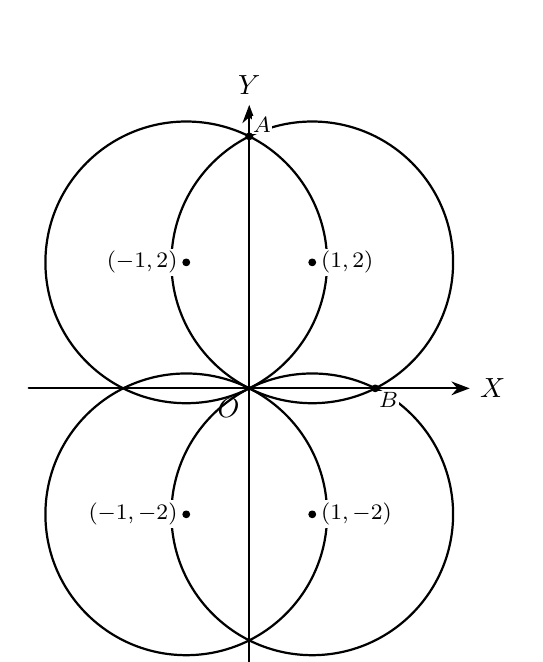
\begin{tikzpicture}[>=Stealth, scale=0.8, line cap=round, line join=round]
  \draw[->, thick] (-3.5, 0) -- (3.5, 0) node[right] {$X$};
  \draw[->, thick] (0, -4.5) -- (0, 4.5) node[above] {$Y$};
  \node[below left] at (0, 0) {$O$};

  % 四個圓心 (1,2), (-1,2), (-1,-2), (1,-2), 半徑 sqrt(5) ~= 2.236
  \draw[thick] (1, 2) circle (2.236);
  \draw[thick] (-1, 2) circle (2.236);
  \draw[thick] (-1, -2) circle (2.236);
  \draw[thick] (1, -2) circle (2.236);

  \filldraw (1, 2) circle (1.5pt) node[right=2pt, fill=white, inner sep=1pt] {\footnotesize $(1,2)$};
  \filldraw (-1, 2) circle (1.5pt) node[left=2pt, fill=white, inner sep=1pt] {\footnotesize $(-1,2)$};
  \filldraw (-1, -2) circle (1.5pt) node[left=2pt, fill=white, inner sep=1pt] {\footnotesize $(-1,-2)$};
  \filldraw (1, -2) circle (1.5pt) node[right=2pt, fill=white, inner sep=1pt] {\footnotesize $(1,-2)$};

  \coordinate (A) at (0, 4);
  \coordinate (B) at (2, 0);
  \filldraw (A) circle (1.5pt) node[above right=1pt, fill=white, inner sep=0.5pt] {\footnotesize $A$};
  \filldraw (B) circle (1.5pt) node[below right=1pt, fill=white, inner sep=0.5pt] {\footnotesize $B$};
\end{tikzpicture}
\caption{四圓相交重疊區域之對稱面積}
\label{fig:b6s-4-prob26}
\end{figure}

\paragraph{【解答】}
在四個象限各有一圓心在 $(\pm 1, \pm 2)$ 半徑為 $\sqrt{5}$ 的圓。兩圓相交之重疊區域面積經計算為 $\dfrac{5\pi}{2}-4$。
故所求總面積為 $4 \times 5\pi - 4\left(\dfrac{5\pi}{2}-4\right) = 2(5\pi+8)$。答案：(甲)。\hfill$\#$

\paragraph{27. （59年度，聯招）}
設 $z$ 為複數，則 $|z-2|+|z+2|=6$ 之解集合在複數平面之圖形為：
\begin{multicols}{2}
\begin{enumerate}[label=\tiangan*]
  \item 相交二直線
  \item 正方形
  \item 圓
  \item 橢圓
  \item 雙曲線
  \item 一直線
\end{enumerate}
\end{multicols}

\paragraph{【解答】}
令 $z=x+iy$，原式即 $\sqrt{(x-2)^2+y^2} + \sqrt{(x+2)^2+y^2} = 6$。
表示點 $(x,y)$ 到兩焦點 $(2,0), (-2,0)$ 之距離和恆為常數 $6 > 4$，故其軌跡為一橢圓。答案：(丁)。\hfill$\#$

\begin{figure}[H]
\centering
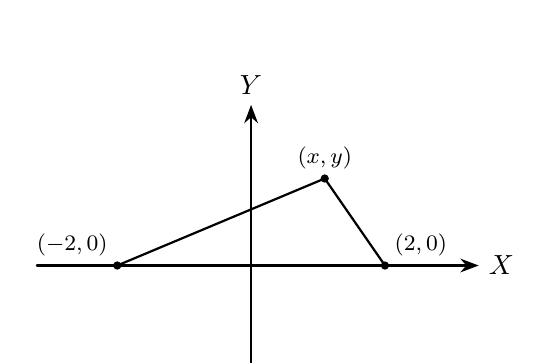
\begin{tikzpicture}[>=Stealth, scale=0.85, line cap=round, line join=round]
  \draw[->, thick] (-3.2, 0) -- (3.4, 0) node[right] {$X$};
  \draw[->, thick] (0, -1.6) -- (0, 2.4) node[above] {$Y$};
  \coordinate (F1) at (-2, 0);
  \coordinate (F2) at (2, 0);
  \coordinate (P) at (1.1, 1.3);
  \draw[thick] (F1) -- (P) -- (F2);
  \filldraw (F1) circle (1.5pt) node[above left] {\footnotesize $(-2,0)$};
  \filldraw (F2) circle (1.5pt) node[above right] {\footnotesize $(2,0)$};
  \filldraw (P) circle (1.5pt) node[above] {\footnotesize $(x,y)$};
\end{tikzpicture}
\end{figure}

\paragraph{28. （59年度，聯招）}
設 $a_n = 1+2+\dots+n$，則無窮級數 $\dfrac{1}{a_1}+\dfrac{1}{a_2}+\dots+\dfrac{1}{a_n}+\dots$ 之和等於多少？

\paragraph{【解答】}
$a_n = \dfrac{n(n+1)}{2} \implies \dfrac{1}{a_n} = \dfrac{2}{n(n+1)} = 2\left(\dfrac{1}{n} - \dfrac{1}{n+1}\right)$。
故
\[ S_n = 2\left[\left(1-\dfrac{1}{2}\right) + \left(\dfrac{1}{2}-\dfrac{1}{3}\right) + \dots + \left(\dfrac{1}{n}-\dfrac{1}{n+1}\right)\right] = 2\left(1-\dfrac{1}{n+1}\right) \longrightarrow 2 \quad (n\to\infty) \text{。}\hfill\# \]

\paragraph{29. （59年度，聯招）}
空間中有二平行線，其方程式分別為
\[ \dfrac{x}{2} = \dfrac{y-1}{1} = \dfrac{z-2}{-1} \quad \text{及} \quad \dfrac{x-1}{2} = \dfrac{y+1}{1} = \dfrac{z-8}{-1} \]
求此二直線之間的距離。

\begin{figure}[H]
\centering
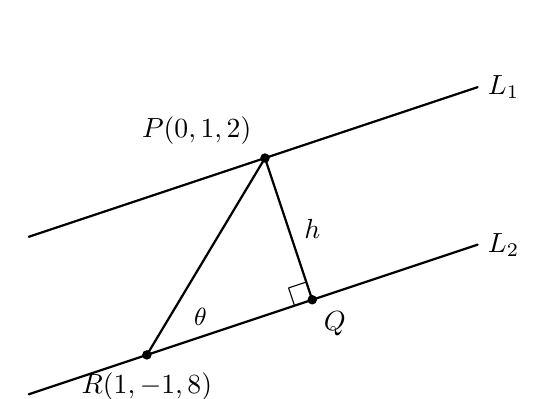
\begin{tikzpicture}[>=Stealth, scale=1.0, line cap=round, line join=round]
  % 兩平行線 L1, L2 (斜率 1/3)
  \draw[thick] (-1.0, 1.6) -- (4.7, 3.5) node[right] {$L_1$};
  \draw[thick] (-1.0, -0.4) -- (4.7, 1.5) node[right] {$L_2$};

  \coordinate (P) at (2.0, 2.6);
  \coordinate (Q) at (2.6, 0.8);
  \coordinate (R) at (0.5, 0.1);

  \draw[thick] (P) -- (Q) node[midway, right=2pt] {$h$};
  \draw[thick] (P) -- (R);

  % 直角記號於 Q (PQ 垂直 L2)
  \draw[thin] ($(Q)+(-0.075,0.225)$) -- ($(Q)+(-0.30,0.15)$) -- ($(Q)+(-0.225,-0.075)$);

  \filldraw (P) circle (1.5pt) node[above left=2pt] {$P(0,1,2)$};
  \filldraw (R) circle (1.5pt) node[below=3pt] {$R(1,-1,8)$};
  \filldraw (Q) circle (1.5pt) node[below right=1pt] {$Q$};
  \node[font=\small] at (1.18, 0.58) {$\theta$};
\end{tikzpicture}
\caption{空間兩平行直線距離幾何投影}
\label{fig:b6s-4-prob29}
\end{figure}

\paragraph{【解答】}
取 $L_1$ 上一點 $P(0,1,2)$，$L_2$ 上一點 $R(1,-1,8)$。方向向量 $\vec{u} = (2,1,-1)$，$\vec{RP} = (-1, 2, -6)$。
\begin{align*}
\cos\theta &= \dfrac{\vec{u}\cdot\vec{RP}}{|\vec{u}||\vec{RP}|} = \dfrac{-2+2+6}{\sqrt{6}\sqrt{41}} = \dfrac{6}{\sqrt{246}}, \\
h &= |\vec{RP}|\sin\theta = \sqrt{41}\sqrt{1-\dfrac{36}{246}} = \sqrt{41}\sqrt{\dfrac{210}{246}} = \sqrt{35} \text{。}\hfill\#
\end{align*}

\paragraph{30. （60年度，聯招）}
以 $x+1$ 除 $6x^3-x^2+2$，所得餘數為：
\begin{multicols}{2}
\begin{enumerate}[label=\tiangan*]
  \item $-5$
  \item $-1$
  \item 2
  \item 3
  \item 7
  \item 9
\end{enumerate}
\end{multicols}

\paragraph{【解答】}
由餘式定理，餘數 $= f(-1) = 6(-1)^3 - (-1)^2 + 2 = -6-1+2 = -5$。答案：(甲)。\hfill$\#$

\paragraph{31. （60年度，聯招）}
設 $\alpha, \beta$ 為二角，並令
\[ \begin{pmatrix} \cos\alpha & -\sin\alpha \\ \sin\alpha & \cos\alpha \end{pmatrix} \begin{pmatrix} \cos\beta & \sin\beta \\ -\sin\beta & \cos\beta \end{pmatrix} = \begin{pmatrix} a & b \\ -a & a \end{pmatrix} \]
則 $b$ 為：
\begin{multicols}{2}
\begin{enumerate}[label=\tiangan*]
  \item $\sin(\alpha+\beta)$
  \item $\cos(\alpha+\beta)$
  \item $\sin(\alpha-\beta)$
  \item $\cos(\alpha-\beta)$
  \item $\sin(\beta-\alpha)$
  \item $-\cos(\beta-\alpha)$
\end{enumerate}
\end{multicols}

\paragraph{【解答】}
由矩陣乘法，第一列第二行元素為：
\[ b = \cos\alpha\sin\beta - \sin\alpha\cos\beta = \sin(\beta-\alpha) \]
答案：(戊)。\hfill$\#$

\paragraph{31*. （60年度，聯招）}\phantomsection\label{note:b6s-ch4-p172-prob-dup}\footnote{【原書註記】：原書此處連續兩題編號皆為 31，本題實為接續之第 32 題，為保持與原書查閱對照之精確性，特加星號註記。}
平面 $x+y+z=4$ 截球面 $(x-1)^2+(y-1)^2+(z-1)^2=1$ 於一圓，此圓之面積為多少？

\begin{figure}[H]
\centering
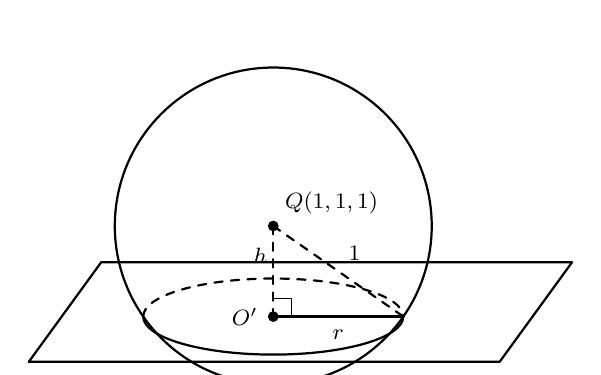
\begin{tikzpicture}[>=Stealth, scale=1.15, line cap=round, line join=round]
  % 球面與平面截圓 (與原書 p.173 一致，放大半徑避免標籤穿線)
  \coordinate (O) at (0, 1.35);
  \draw[thick] (O) circle (1.75);
  \filldraw (O) circle (1.5pt) node[above right=1pt, font=\footnotesize] {$Q(1,1,1)$};

  % 截面橢圓 (y=0.35, 半長軸 sqrt(1.75^2 - 1^2) = 1.436)
  \coordinate (Oprime) at (0, 0.35);
  \coordinate (A) at (1.436, 0.35);
  \draw[thick] (-1.436, 0.35) arc (180:360:1.436 and 0.42);
  \draw[thick, dashed] (-1.436, 0.35) arc (180:0:1.436 and 0.42);
  \filldraw (Oprime) circle (1.5pt) node[left=2pt, font=\footnotesize] {$O'$};

  \draw[thick, dashed] (O) -- (Oprime);
  \node[left=1.5pt, fill=white, inner sep=0.5pt, font=\footnotesize] at (0, 1.02) {$h$};
  \draw[thick, dashed] (O) -- (A) node[midway, above right, font=\footnotesize] {$1$};
  \draw[thick] (Oprime) -- (A) node[midway, below=1pt, font=\footnotesize] {$r$};
  % 直角記號
  \draw[thin] (0, 0.55) -- (0.20, 0.55) -- (0.20, 0.35);

  % 平面示意
  \draw[thick] (-2.7, -0.15) -- (2.5, -0.15) -- (3.3, 0.95) -- (-1.9, 0.95) -- cycle;
\end{tikzpicture}
\caption{平面截球面所成圓面積之立體幾何模型}
\label{fig:b6s-4-prob31bis}
\end{figure}

\paragraph{【解答】}
\begin{enumerate}[label=(\arabic*), leftmargin=2em]
  \item 球心 $Q(1,1,1)$ 至平面 $x+y+z-4=0$ 的距離：
  \[ h = \dfrac{|1+1+1-4|}{\sqrt{1+1+1}} = \dfrac{1}{\sqrt{3}} \]
  \item 圓的半徑 $r = \sqrt{1^2-h^2} = \sqrt{1-\dfrac{1}{3}} = \sqrt{\dfrac{2}{3}}$。
  \item 圓之面積為 $\pi r^2 = \dfrac{2}{3}\pi$。\hfill$\#$
\end{enumerate}

\paragraph{32. （61年度，聯招）}
聯立不等式
\[ \begin{cases} 0 < x < 2\pi \\ \sin x \cos^3 x > \sin^3 x \cos x \end{cases} \]
之解集合為：

\paragraph{【解答】}
$\sin x \cos x(\cos^2 x - \sin^2 x) > 0 \implies \dfrac{1}{2}\sin 2x \cos 2x > 0 \implies \dfrac{1}{4}\sin 4x > 0$。
故 $2n\pi < 4x < (2n+1)\pi \implies \dfrac{n\pi}{2} < x < (2n+1)\dfrac{\pi}{4}$。
在 $0<x<2\pi$ 內，解集合為：
\[ 0 < x < \dfrac{\pi}{4}, \quad \dfrac{\pi}{2} < x < \dfrac{3\pi}{4}, \quad \pi < x < \dfrac{5\pi}{4}, \quad \dfrac{3\pi}{2} < x < \dfrac{7\pi}{4} \text{。}\hfill\# \]

\paragraph{33. （61年度，聯招）}
下表係錄自60年度綜合所得稅申報表中之一段：

\begin{center}
\textbf{第一表\quad 綜合所得稅稅率表}

\small
\renewcommand{\arraystretch}{1.2}
\begin{tabular}{|c|l|c|}
\hline
級別 & 級\qquad 距 & 稅率 \\ \hline
1 & 綜合所得淨額在 3 萬元以下的 & $6\%$ \\
2 & 綜合所得淨額超過 3 萬元到 6 萬元之間的 & $8\%$ \\
3 & 綜合所得淨額超過 6 萬元到 10 萬元之間的 & $10\%$ \\
4 & 綜合所得淨額超過 10 萬元到 15 萬元之間的 & $12\%$ \\ \hline
\end{tabular}

\vspace{0.8em}
\textbf{第二表\quad 速算公式表}

\begin{tabular}{|c|r@{\ }c@{\ }l|}
\hline
級別 & \multicolumn{3}{c|}{綜合所得淨額 $\times$ 稅率 $-$ 累進差額 $=$ 全年應納稅額} \\ \hline
1 & 綜合所得淨額 $\times 0.06$ & $-$ & $0$ 元 $=$ 全年應納稅額 \\
2 & 綜合所得淨額 $\times 0.08$ & $-$ & $600$ 元 $=$ 全年應納稅額 \\
3 & 綜合所得淨額 $\times 0.10$ & $-$ & $1800$ 元 $=$ 全年應納稅額 \\
4 & 綜合所得淨額 $\times 0.12$ & $-$ & $3800$ 元 $=$ 全年應納稅額 \\ \hline
\end{tabular}
\end{center}

今設綜合所得淨額為 $x$，全年應納所得稅額為 $y$，則 $y$ 為 $x$ 的函數。
\begin{enumerate}[label=\arabic*), leftmargin=2em]
  \item 根據第一表將各級之 $x, y$ 的關係式分別列出。
  \item 由此結果導出第二表的速算公式。
  \item 將第一級到第 4 級 $x, y$ 間的關係用單一個式子表示出來。
\end{enumerate}

\paragraph{【解答】}
\begin{enumerate}[label=\arabic*), leftmargin=2em]
  \item 
  \begin{align*}
  \text{在 } 0\le x\le 30000: &\quad y = x \times 0.06 \tag{1} \\
  \text{在 } 30000 < x \le 60000: &\quad y = (x-30000)\times 0.08 + 30000\times 0.06 \tag{2} \\
  \text{在 } 60000 < x \le 100000: &\quad y = (x-60000)\times 0.10 + 30000\times 0.08 + 30000\times 0.06 \tag{3} \\
  \text{在 } 100000 < x \le 150000: &\quad y = (x-100000)\times 0.12 + 40000\times 0.10 \\
  &\quad\quad + 30000\times 0.08 + 30000\times 0.06 \tag{4}
  \end{align*}
  \item 
  從 (1): $y = x\times 0.06 - 0$ 為第一級\\
  從 (2): $y = x\times 0.08 - 600$ 為第二級\\
  從 (3): $y = x\times 0.10 - 1800$ 為第三級\\
  從 (4): $y = x\times 0.12 - 3800$ 為第四級
  \item 令函數為
  \[ y = ax + b|x-30000| + c|x-60000| + d|x-100000| + e \]
  經分段比較係數，解得
  \[ a=0.09, \quad b=0.01, \quad c=0.01, \quad d=0.01, \quad e=-1900 \]
  故原方程式為
  \[ y = 0.09x + 0.01|x-30000| + 0.01|x-60000| + 0.01|x-100000| - 1900 \text{。}\hfill\# \]
\end{enumerate}

\begin{center}
\textbf{63 年聯考（甲丙組）}
\end{center}

\paragraph{1. （63年度，聯招）}
設 $m, n$ 為任意正整數，且 $m>n$。令 $x=m^2-n^2, y=2mn, z=m^2+n^2$。譬如說 $m=2, n=1$，則 $x=3, y=4, z=5$，而下列各敘述成立。今問其中那些敘述在一般情形恆成立？
\begin{multicols}{2}
\begin{enumerate}[label=(\Alph*)]
  \item $x < y$
  \item $x+y > z$
  \item $x, y$ 中必有一數為 4 之倍數
  \item $x, y$ 中必有一數為 3 之倍數
  \item $x, y, z$ 中必有一數為 5 之倍數
\end{enumerate}
\end{multicols}

\paragraph{【解答】}
(B), (C), (D), (E) 為真。（第一冊，第三章）。\hfill$\#$

\paragraph{2. （63年度，聯招）}
三直線 $x-y-9=0, x+2y=0$ 及 $3x-y-7=0$ 圍成一三角形，設此三角形外接圓的方程式為 $x^2+y^2+ax+by+c=0$，則
\begin{multicols}{2}
\begin{enumerate}[label=(\Alph*)]
  \item 此三角形的三個頂點都在第四象限
  \item $a+b=8$
  \item $2a-b=20$
  \item 外接圓圓心的坐標為 $(2, -6)$
  \item $a^2+b^2-4c=100$
\end{enumerate}
\end{multicols}

\paragraph{【解答】}
解出三直線的交點為 $(6,-3), (-1,-10), (2,-1)$。代入圓方程式得：
\[ a = -4, \quad b = 12, \quad c = 15 \]
圓心為 $(2, -6)$，$a+b = 8$，$a^2+b^2-4c = 16+144-60 = 100$。
答案：(B), (D), (E) 為真。（第六冊，第一章；第四冊，第三章）。\hfill$\#$

\paragraph{3. （63年度，聯招）}
考慮如右的街道圖，其中 $A, B, C, D$ 為四邊站。警察在巡邏時，必須走過所有的街道，但是不重複走過同一條街，因此派出所只能設在 $A$ 站或 $D$ 站。從 $A$ 站出發要完成一次巡邏，可以有 $N$ 個不同路線（試求出 $N$），則
\begin{multicols}{2}
\begin{enumerate}[label=(\Alph*)]
  \item $N$ 可被 25 整除
  \item $N$ 可被 45 整除
  \item $N$ 可被 48 整除
  \item $N$ 可被 160 整除
  \item $N > 700$
\end{enumerate}
\end{multicols}

\begin{figure}[H]
\centering
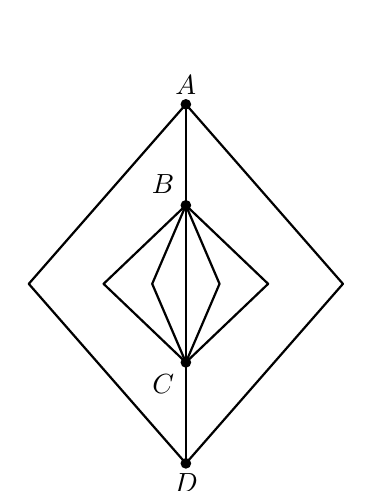
\begin{tikzpicture}[>=Stealth, scale=0.95, line cap=round, line join=round]
  % 依原書 p.178 精確繪製多層菱形歐拉圖
  \coordinate (A) at (0, 2.4);
  \coordinate (B) at (0, 1.05);
  \coordinate (C) at (0, -1.05);
  \coordinate (D) at (0, -2.4);
  \coordinate (L1) at (-2.1, 0);
  \coordinate (R1) at (2.1, 0);
  \coordinate (L2) at (-1.1, 0);
  \coordinate (R2) at (1.1, 0);
  \coordinate (L3) at (-0.45, 0);
  \coordinate (R3) at (0.45, 0);

  \draw[thick] (A) -- (L1) -- (D) -- (R1) -- cycle;
  \draw[thick] (B) -- (L2) -- (C) -- (R2) -- cycle;
  \draw[thick] (B) -- (L3) -- (C) -- (R3) -- cycle;
  \draw[thick] (A) -- (D);

  \filldraw (A) circle (1.8pt) node[above] {$A$};
  \filldraw (B) circle (1.8pt) node[above left=1pt] {$B$};
  \filldraw (C) circle (1.8pt) node[below left=1pt] {$C$};
  \filldraw (D) circle (1.8pt) node[below] {$D$};
\end{tikzpicture}
\caption{警察巡邏路線圖（歐拉圖）}
\label{fig:b6s-4-prob-patrol}
\end{figure}

\paragraph{【解答】}
$N = 6! = 720$。故 (C), (E) 為真。（第五冊，第二章）。\hfill$\#$


% ==========================================
% 附錄 IV\quad 導數 (pp. 179-214)
% ==========================================
\newpage
\phantomsection
\section*{附錄 IV\quad 導數}\label{sec:b6s-app4}
\addcontentsline{toc}{section}{\texorpdfstring{附錄 IV\quad 導數}{附錄 IV 導數}}
\resetsectcounters

\begin{itemize}[leftmargin=3em, itemsep=0.2em]
  \item[§ 1] \textbf{函數與極限}
  \item[§ 2] \textbf{導函數}
  \begin{itemize}[leftmargin=2em, itemsep=0.1em]
    \item[甲、] 變率和導數
    \item[乙、] 導函數
  \end{itemize}
  \item[§ 3] \textbf{幾個基本函數的微分}
  \begin{itemize}[leftmargin=2em, itemsep=0.1em]
    \item[甲、] 三角函數的導函數
    \item[乙、] 指數函數與對數函數
    \item[丙、] 高階導函數
  \end{itemize}
  \item[§ 4] \textbf{函數圖形}
  \begin{itemize}[leftmargin=2em, itemsep=0.1em]
    \item[甲、] 切線方程式
    \item[乙、] 極大極小
  \end{itemize}
  \item[§ 5] \textbf{近似值}
  \begin{itemize}[leftmargin=2em, itemsep=0.1em]
    \item[甲、] 均值定理與泰勒公式
    \item[乙、] 牛頓式求根法
  \end{itemize}
  \item[§ 6] \textbf{導數與面積}
\end{itemize}

\begin{center}
$* \qquad * \qquad * \qquad * \qquad *$
\end{center}

\phantomsection
\subsection*{§ 1\quad 函數與極限}\label{subsec:b6s-app4-1}
\addcontentsline{toc}{subsection}{\texorpdfstring{§ 1\quad 函數與極限}{§ 1 函數與極限}}

在第一冊第五章裡，我們討論了函數的涵義，在第二冊第二章我們又討論了數列和數列的極限，其實數列就是由自然數集合到實數集合的函數。所以，是一種函數的特例。因此，很自然地我們就可以考慮到一般函數的極限觀念。

\begin{example}\label{ex:b6s-app4-1}
令 $f: \mathbb{R}\to\mathbb{R}$ 定義如下：
\[ f(x) = 1+x \]
則它的圖形如圖 1-1。顯然，當 $x$ 不管從左或從右趨近於 0 時，$y$ 就會趨近於 1。

在這種情形，仿照數列極限的定義，我們就說當 $x$ 趨近於 0 時，函數 $f$ 的極限為 1，記作
\[ \lim_{x\to 0} f(x) = 1 \]
\end{example}

\begin{example}\label{ex:b6s-app4-2}
設函數 $f: \mathbb{R}\to\mathbb{R}$ 由下式定義：
\[ f(x) = |x-1| \]
則它的圖示如右（圖 1-2）。顯然，當 $x$ 趨近於 1 時，$y$ 趨近於 0。因此，當 $x$ 趨近於 1 時函數 $f$ 的極限為 0，$\lim_{x\to 1} f(x) = 0$。
\end{example}

\begin{figure}[H]
\centering
\begin{subfigure}[b]{0.45\textwidth}
\centering
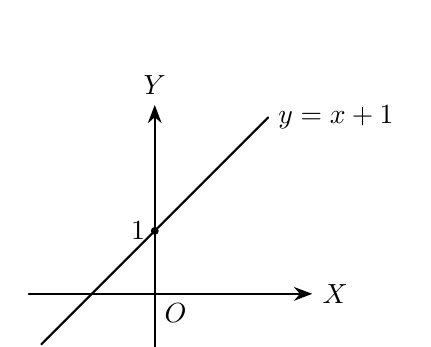
\begin{tikzpicture}[>=Stealth, scale=0.8, line cap=round]
  \draw[->, thick] (-2, 0) -- (2.5, 0) node[right] {$X$};
  \draw[->, thick] (0, -1) -- (0, 3) node[above] {$Y$};
  \node[below right] at (0, 0) {$O$};
  \draw[thick] (-1.8, -0.8) -- (1.8, 2.8) node[right] {$y=x+1$};
  \filldraw (0, 1) circle (1.5pt) node[left] {$1$};
\end{tikzpicture}
\caption{圖 1-1}
\end{subfigure}
\begin{subfigure}[b]{0.45\textwidth}
\centering
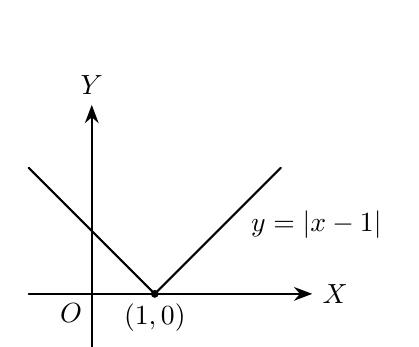
\begin{tikzpicture}[>=Stealth, scale=0.8, line cap=round]
  \draw[->, thick] (-1, 0) -- (3.5, 0) node[right] {$X$};
  \draw[->, thick] (0, -1) -- (0, 3) node[above] {$Y$};
  \node[below left] at (0, 0) {$O$};
  \draw[thick] (-1, 2) -- (1, 0) -- (3, 2);
  \node[right=4pt] at (2.2, 1.1) {$y=|x-1|$};
  \filldraw (1, 0) circle (1.5pt) node[below] {$(1,0)$};
\end{tikzpicture}
\caption{圖 1-2}
\end{subfigure}
\caption{函數極限直觀圖示}
\label{fig:b6s-app4-limit-intro}
\end{figure}

對於任意函數 $f: A\to B$，當 $x$ 趨近 $a$ 於時，$f(x)$ 趨近於 $b$，則稱 $x$ 趨近於 $a$ 時函數 $f$ 的極限為 $b$，記為 $\lim_{x\to a} f(x) = b$。

這就是說，當 $x$ 無限逼近於 $a$ 時，$f(x)$ 就會無限的逼近於 $b$。換一種方式講，就是說，對任意靠近 $b$ 的範圍內，只要 $x$ 相當接近 $a$，$f(x)$ 就會在這個 $b$ 的臨近範圍內。這些話可用數學符號表示如下：
\[ \text{對於任意的 } \varepsilon > 0, \text{ 一定存在 } \delta > 0 \text{ 使得 } |x-a| < \delta \implies |f(x)-b| < \varepsilon \]

上面這種嚴格的定義，在現階段我們不須要去強調它。我們只要接受「當 $x$ 趨近於 $a$ 時，$f(x)$ 趨近於 $b$，就說 $\lim_{x\to a} f(x) = b$」這個觀念就足夠了。

\begin{example}\label{ex:b6s-app4-3}
求 $\lim_{x\to 2} \dfrac{x^2-4}{x-2}$。
\end{example}

\paragraph{【解】}
若 $f(x) = \dfrac{x^2-4}{x-2}$，當 $x=2$ 時，我們從式中不知道 $f(2)$ 等於多少。但我們知道，對於 $x\ne 2$ 的實數，
\[ f(x) = \dfrac{x^2-4}{x-2} = x+2 \]
所以，當 $x\longrightarrow 2$ 時，$f(x)\longrightarrow 4$，因此 $\lim_{x\to 2}\dfrac{x^2-4}{x-2} = 4$。\hfill$\#$

\begin{example}\label{ex:b6s-app4-4}
求 $\lim_{x\to 0} x\sin\dfrac{1}{x}$。
\end{example}

\paragraph{【解】}
當 $x$ 趨近於 0 時，因為 $\sin\dfrac{1}{x}$ 是一週期函數 $\sin\dfrac{1}{x}$ 在 $-1$ 與 1 之間變動，但無論如何 $\left|\sin\dfrac{1}{x}\right| \le 1$，因此
\[ \left|x\sin\dfrac{1}{x}\right| \le |x| \]
所以當 $x\longrightarrow 0$ 時，$\left|x\sin\dfrac{1}{x}\right|\longrightarrow 0$，因此
\[ \lim_{x\to 0} x\sin\dfrac{1}{x} = 0 \text{。}\hfill\# \]

並不是所有的極限都會存在，下面就是一個例子。

\begin{example}\label{ex:b6s-app4-5}
求 $\lim_{x\to 0}\dfrac{|x|}{x}$。
\end{example}

\paragraph{【解】}
我們先看看 $f(x) = \dfrac{|x|}{x}$ 的圖形，當 $x>0$ 時，$|x|=x$，因此 $f(x) = 1$；當 $x<0$ 時，$|x|=-x$，所以 $f(x) = -1$。

\begin{figure}[H]
\centering
\begin{tikzpicture}[>=Stealth, scale=0.9, line cap=round]
  \draw[->, thick] (-2.5, 0) -- (2.5, 0) node[right] {$X$};
  \draw[->, thick] (0, -2) -- (0, 2) node[above] {$Y$};
  \node[below right] at (0, 0) {$O$};

  \draw[line width=1.5pt] (0.05, 1) -- (2.2, 1);
  \draw (0, 1) circle (2pt);
  \draw[line width=1.5pt] (-2.2, -1) -- (-0.05, -1);
  \draw (0, -1) circle (2pt);
\end{tikzpicture}
\caption{圖 1-3\quad 符號函數 $\dfrac{|x|}{x}$ 之跳躍不連續圖形}
\label{fig:b6s-app4-signum}
\end{figure}

其圖如圖 1-3，可見當 $x$ 從左（小於 0）趨近於 0 時，$\dfrac{|x|}{x}$ 趨近於 $-1$，而當 $x$ 從右（大於 0）趨近於 0 時，$\dfrac{|x|}{x}$ 趨近於 1。因此我們不能說：當 $x$ 趨近於 0 時，$\dfrac{|x|}{x}$ 趨近於某一固定實數，所以 $\lim_{x\to 0}\dfrac{|x|}{x}$ 不存在。\hfill$\#$

如同數列的極限一樣，函數的極限有下述的性質：如果 $f, g$ 為兩個函數，且 $\lim_{x\to a} f(x)$ 和 $\lim_{x\to a} g(x)$ 都存在，則 $\lim_{x\to a}(f(x)\pm g(x))$，$\lim_{x\to a}(f(x)g(x))$ 存在，而且：
\begin{enumerate}[label=\Roman*., leftmargin=2em]
  \item $\lim_{x\to a}(f(x)+g(x)) = \lim_{x\to a}f(x) + \lim_{x\to a}g(x)$
  \item $\lim_{x\to a}(f(x)-g(x)) = \lim_{x\to a}f(x) - \lim_{x\to a}g(x)$
  \item $\lim_{x\to a}(f(x)g(x)) = \lim_{x\to a}f(x) \cdot \lim_{x\to a}g(x)$
  \item 如果再加上條件：$\lim_{x\to a}g(x)\ne 0$，則 $\lim_{x\to a}\dfrac{f(x)}{g(x)}$ 存在，而且
  \[ \lim_{x\to a}\dfrac{f(x)}{g(x)} = \dfrac{\lim_{x\to a}f(x)}{\lim_{x\to a}g(x)} \]
  \item 如果 $\sqrt[n]{\lim_{x\to a}f(x)}$ 有意義（有定義）時，則 $\lim_{x\to a}\sqrt[n]{f(x)}$ 存在，而且
  \[ \lim_{x\to a}\sqrt[n]{f(x)} = \sqrt[n]{\lim_{x\to a}f(x)} \]
\end{enumerate}

這些性質表明了，在“良好”的情況下，函數間相加減乘數或開根號的運算可以與取極限的運算互換。

這些等式我們不做嚴密的證明，只要知道如何應用就可以了。

\begin{discussion}\label{ex:b6s-app4-disc1}\label{disc:b6s-app4-1}
令 $f(x) = a_0 + a_1 x + \dots + a_n x^n$，則
\begin{align*}
\lim_{x\to a} f(x) &= \lim_{x\to a}(a_0 + a_1 x + \dots + a_n x^n) \\
&= \lim_{x\to a}a_0 + \lim_{x\to a}a_1 x + \dots + \lim_{x\to a}a_n x^n \\
&= \lim_{x\to a}a_0 + \lim_{x\to a}a_1\lim_{x\to a}x + \dots + \lim_{x\to a}a_n\left(\lim_{x\to a}x\right)^n \\
&= a_0 + a_1 a + \dots + a_n a^n
\end{align*}
\end{discussion}

\begin{example}\label{ex:b6s-app4-6}
試求 $\lim_{x\to 2} \dfrac{x-2}{\sqrt{x^2-4}}$。
\end{example}

\paragraph{【解】}
\begin{align*}
\lim_{x\to 2} \dfrac{x-2}{\sqrt{x^2-4}} &= \lim_{x\to 2}\dfrac{(\sqrt{x-2})^2}{\sqrt{x-2}\sqrt{x+2}} = \lim_{x\to 2}\dfrac{\sqrt{x-2}}{\sqrt{x+2}} \\
&= \lim_{x\to 2}\sqrt{\dfrac{x-2}{x+2}} = 0
\end{align*}
因為 $\lim_{x\to 2}\dfrac{x-2}{x+2} = 0$。\hfill$\#$

\subsubsection*{習題 1}\label{sec:b6s-ex-app4-1}

\begin{enumerate}[label=\arabic*., leftmargin=2em]
  \item 試求下列各極限：
  \begin{multicols}{2}
  \begin{enumerate}[label=(\arabic*)]
    \item $\lim_{x\to 1}(1+x+x^2)$
    \item $\lim_{x\to 4}(1+\sqrt{x}+x^2)$
    \item $\lim_{x\to 1}\dfrac{x^3-2x^2+1}{x-1}$
    \item $\lim_{x\to 1}\dfrac{\sqrt{1-x^2}}{\sqrt{1-x}}$
    \item $\lim_{x\to 1}\dfrac{x^3-x^2-x+1}{x^2+x-2}$
    \item $\lim_{x\to 0}(\sqrt{a+x}+\sqrt{a-x})$
    \item $\lim_{x\to 0}\dfrac{x}{\sqrt{1+x}-\sqrt{1-x}}$
    \item $\lim_{x\to 1}\dfrac{x-1}{\sqrt[3]{x}-1}$
    \item $\lim_{x\to 0}x\cos\dfrac{1}{x}$
    \item $\lim_{x\to 1}\dfrac{x-1}{x}\sin\dfrac{1}{x-1}$
  \end{enumerate}
  \end{multicols}

  \item 令 $[x]$ 表示小於或等於 $x$ 的最大整數，試問
  \[ \lim_{x\to 1}[x] \text{ 是否存在？} \qquad \lim_{x\to 0.5}[x] \text{ 是否存在？} \]

  \item 將 $x$ 看做常數，試求：
  \[ \lim_{h\to 0}\dfrac{2(x+h)^2 - 5(x+h)^3 - 2x^2 - 5x^3}{h} \]

  \item 令 $f(x)=x^2$，試證 $\lim_{h\to 0}\dfrac{f(x+h)-f(x)}{h} = 2x$。

  \item 問 $a$ 為何值時，$\lim_{x\to 1}\dfrac{x^2-6x+a}{x^2+2x-3}$ 有極限？它的極限是多少？
\end{enumerate}

\phantomsection
\subsection*{§ 2\quad 導函數}\label{subsec:b6s-app4-2}
\addcontentsline{toc}{subsection}{\texorpdfstring{§ 2\quad 導函數}{§ 2 導函數}}
\setcounter{theorem}{0}
\renewcommand{\thetheorem}{2.\arabic{theorem}}

\subsubsection*{甲、變率和導數}

數學上，我們用函數來描示事物的狀態和幾何圖形，對於事物的狀態和幾何圖形我們常須了解它的變動情形。

下表是縱貫鐵路光華號 2001 次列車所停各站的時刻和該站與基隆的距離：

\begin{center}
\textbf{表 2-1}

\renewcommand{\arraystretch}{1.2}
\begin{tabular}{|c|c|c|c|c|c|c|}
\hline
站名 & 基隆 & 臺北 & 臺中 & 臺南 & 高雄 & 屏東 \\ \hline
時間 & 6.17 & 7.00 & 9.32 & 11.28 & 12.10 & 12.34 \\ \hline
距離 & 0 & 28.6 & 197.4 & 357.5 & 404.2 & 425.1 \\ \hline
\end{tabular}
\end{center}

現在以 $x$ 代表時間，$y=f(x)$ 表示在時間為 $x$ 時，該列車與基隆的距離則由表記：
\begin{align*}
f(7.00) &= 28.6 \qquad (\text{在臺北站}) \\
f(9.32) &= 197.4 \qquad (\text{在臺中站}) \\
&\ \ \vdots \\
f(12.34) &= 425.1 \qquad (\text{在屏東站})
\end{align*}
注意上面的 $x$ 值並非十進位數！函數 $f$ 描述了該列車行駛狀態，由 $f$，我們知道該列，從基隆到屏東所須時間為 6.28 小時（$\doteq 6$ 小時 17 分）所以，它平均每小時走 $\dfrac{425.1}{6.28} = 67.69$ 公里，我們說這是它的平均速率，在數學上，我們稱它為\textbf{平均變率}。

當函數 $y=f(x)$ 在線段 $[a, b] = \{x; a\le x\le b\}$ 上定義時，比值 $\dfrac{f(b)-f(a)}{b-a}$ 叫做函數 $y=f(x)$ 在 $a, b$ 間的平均變率。如下圖所示，平均變率，其實就是線段 $\overline{P_a P_b}$ 的斜率。

\begin{figure}[H]
\centering
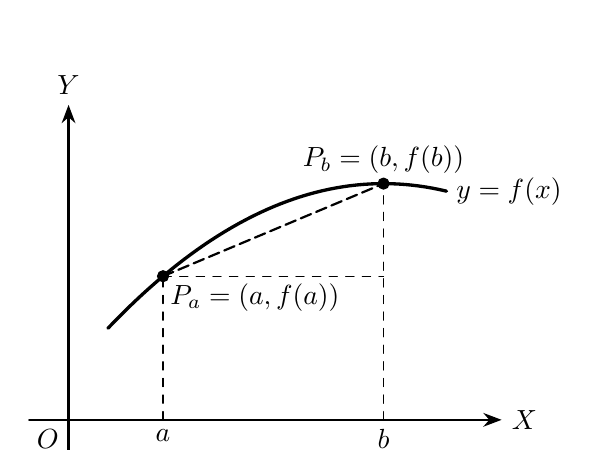
\begin{tikzpicture}[>=Stealth, scale=1.0, line cap=round, line join=round]
  \draw[->, thick] (-0.5, 0) -- (5.5, 0) node[right] {$X$};
  \draw[->, thick] (0, -0.5) -- (0, 4.0) node[above] {$Y$};
  \node[below left] at (0, 0) {$O$};

  % 曲線 y = f(x)
  \draw[line width=1.2pt, domain=0.5:4.8, samples=50] plot (\x, {0.6 + 1.2*\x - 0.15*\x*\x});
  \node[right] at (4.8, 2.9) {$y=f(x)$};

  \coordinate (Pa) at (1.2, 1.824);
  \coordinate (Pb) at (4.0, 3.0);

  \draw[thick, dash pattern=on 4pt off 2pt] (Pa) -- (Pb);
  \draw[dashed] (1.2, 0) node[below] {$a$} -- (Pa);
  \draw[dashed] (4.0, 0) node[below] {$b$} -- (Pb);
  \draw[dashed] (Pa) -- (4.0, 1.824);

  \filldraw (Pa) circle (2pt) node[below right=2pt, fill=white, inner sep=1pt] {$P_a=(a, f(a))$};
  \filldraw (Pb) circle (2pt) node[above] {$P_b=(b, f(b))$};
\end{tikzpicture}
\caption{圖 2-1\quad 平均變率之幾何意義（割線斜率）}
\label{fig:b6s-app4-avg-rate}
\end{figure}

對於等速運動來說，取任意時間內的平均速率都相等。但對上例的火車來說，平均速率並不能代表該列車在任意時刻走的快慢。這很容易從表中驗算比較得來。

\subsubsection*{作業 1}
試計算下列各站間，2001 次光華號的平均速率：
\begin{enumerate}[label=\alph*., leftmargin=2em]
  \item 臺北與臺南間
  \item 臺中與高雄間
\end{enumerate}

物理學告訴我們，要看一物體運動的快慢，必需用每瞬間的快慢來衡量，如以光華號車為例，該車在 10 時正行駛快慢的程度，應以 10 時到 10 時 01 分所走的路程，或甚至更短時間 $\Delta t$ 所走的路程的平均速率才能表示它的快慢，而且 $\Delta t$ 越逼近於 0 的平均速率越能表示該時刻的速率，以此推之於函數的變動情形，我們有如下的觀念：

\begin{definition*}[導數（變率）的定義]\label{def:b6s-app4-derivative}
對於一個固定的 $a$，假如平均變率 $\dfrac{f(b)-f(a)}{b-a}$ 在 $b\to a$ 時有一個極限值，即 $\lim_{b\to a}\dfrac{f(b)-f(a)}{b-a}$ 存在，則稱這種極限為 $y=f(x)$ 在 $x=a$ 時的\textbf{瞬間變率}又稱為函數 $f(x)$ 在 $x=a$ 的\textbf{導數}。
\end{definition*}

平常為了明示 $a$ 為固定，而 $b\to a$，我們改用 $b=a+h$（即 $h=b-a$）則 $y=f(x)$ 在 $x=a$ 的導數為
\[ \lim_{h\to 0}\dfrac{f(a+h)-f(a)}{h} \]
我們將 $f(x)$ 在 $x=a$ 的導數記為 $\left.\dfrac{df}{dx}\right|_a$，又記為 $f'(a)$。

\paragraph{注意：}
\begin{enumerate}[label=(\roman*), leftmargin=2em]
  \item $h$ 是可正可負的。
  \item 當上述極限不存在時，我們說 $y=f(x)$ 在點 $x=a$ 無導數。
  \item 由上節所定義的極限觀念，不難看出函數 $f$ 在 $x=a$ 連續的充分必要條件為 $\lim_{x\to a}f(x) = f(a)$。如果 $f$ 在 $x=a$ 有導數 $f'(a)$，則
  \begin{align*}
  \lim_{x\to a}[f(x)-f(a)] &= \lim_{x\to a}\left[\dfrac{f(x)-f(a)}{x-a}(x-a)\right] \\
  &= \lim_{x\to a}\dfrac{f(x)-f(a)}{x-a}\lim_{x\to a}(x-a) = 0
  \end{align*}
  所以 $f$ 在 $x=a$ 連續。
\end{enumerate}

這種求函數在某點的導數的手段叫做\textbf{微分}。函數 $f(x)$ 在 $x=a$ 有導數時，稱 $f(x)$ 在 $x=a$ 可微分或可微又可說 $f(x)$ 在 $x=a$ 處是平滑的，否則稱為在 $x=a$ 不可微分或不可微。

\begin{example}\label{ex:b6s-app4-7}
求 $f(x)=cx+d$ 在 $x=a$ 的導數。
\end{example}

\paragraph{【解】}
\[ f'(a) = \lim_{h\to 0}\dfrac{f(a+h)-f(a)}{h} = \lim_{h\to 0}\dfrac{[c(a+h)+d]-[ca+d]}{h} = c \]
所以 $f(x)=cx+d$，在任意點 $x=a$ 的導數都為常數 $c$。這由 $y=f(x)$ 的圖形很容易看出來，因為它的圖形是直線，所以圖上任意兩點連線的斜率為常數。\hfill$\#$

\begin{example}\label{ex:b6s-app4-8}
試求 $y=x^2$ 在 $x=a$ 時的導數。
\end{example}

\paragraph{【解】}
因為 $f(a+h) = (a+h)^2 = a^2+2ah+h^2$，$f(a+h)-f(a) = 2ah+h^2$。
所以 $f'(a) = \lim_{h\to 0}\dfrac{2ah+h^2}{h} = 2a$。\hfill$\#$

\begin{example}\label{ex:b6s-app4-9}
試求 $y=x^n$ 在 $x=a$ 時的導數。
\end{example}

\paragraph{【解】}
\begin{align*}
f'(a) &= \lim_{h\to 0}\dfrac{(a+h)^n - a^n}{h} = \lim_{h\to 0}\dfrac{na^{n-1}h + {}_n C_2 a^{n-2}h^2 + \dots + h^n}{h} \quad (\text{二項式定理展開}) \\
&= na^{n-1} \text{。}\hfill\#
\end{align*}

\begin{example}\label{ex:b6s-app4-10}
設 $f(x)=|x|$，求 $f(x)$ 在 $x=0$ 的導數。
\end{example}

\paragraph{【解】}
當 $h>0$ 時，$\dfrac{f(0+h)-f(0)}{h} = \dfrac{h}{h} = 1$；故當 $h$ 從右邊（大於 0）趨近於 0 時，$\dfrac{f(0+h)-f(0)}{h}$ 趨近於 1。
當 $h<0$ 時，$\dfrac{f(0+h)-f(0)}{h} = -1$，故當 $h$ 從左（小於 0）趨近於 0 時，$\dfrac{f(0+h)-f(0)}{h}$ 趨近於 $-1$。所以當 $h$ 趨近於 0 時，$\dfrac{f(0+h)-f(0)}{h}$ 不能趨近於一固定數，就是說 $\lim_{h\to 0}\dfrac{f(0+h)-f(0)}{h}$ 不存在。所以 $f(x)=|x|$ 在 $x=0$ 無導數。\hfill$\#$

\begin{figure}[H]
\centering
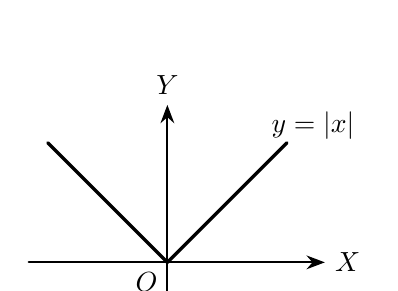
\begin{tikzpicture}[>=Stealth, scale=0.8, line cap=round, line join=round]
  \draw[->, thick] (-2.2, 0) -- (2.5, 0) node[right] {$X$};
  \draw[->, thick] (0, -0.6) -- (0, 2.5) node[above] {$Y$};
  \node[below left] at (0, 0) {$O$};
  \draw[line width=1.2pt] (-1.9, 1.9) -- (0, 0) -- (1.9, 1.9);
  \node[above right] at (1.5, 1.8) {$y=|x|$};
\end{tikzpicture}
\end{figure}

\begin{example}\label{ex:b6s-app4-11}
令 $x\ge 0, f(x)=\sqrt{x}$，試求 $f(x)$ 在 $x=a\ (>0)$ 時的導數。
\end{example}

\paragraph{【解】}
對任意 $x=a>0$，取 $|h|$ 相當小時，$a+h>0$，所以 $\sqrt{a+h}$ 有意義，而且
\[ \dfrac{\sqrt{a+h}-\sqrt{a}}{h} = \dfrac{a+h-a}{h(\sqrt{a+h}+\sqrt{a})} = \dfrac{1}{\sqrt{a+h}+\sqrt{a}} \]
所以 $f'(a) = \lim_{h\to 0}\dfrac{f(a+h)-f(a)}{h} = \lim_{h\to 0}\dfrac{1}{\sqrt{a+h}+\sqrt{a}} = \dfrac{1}{2\sqrt{a}}$。\hfill$\#$

\subsubsection*{作業 2}
當 $x=0$ 時，$f(x)=\sqrt{x}$ 的導數為何？有無意義？

\subsubsection*{習題 2-A}\label{sec:b6s-ex-app4-2a}

\begin{enumerate}[label=\arabic*., leftmargin=2em]
  \item 試求下列各函數在 $x=a$ 時的導數：
  \begin{multicols}{2}
  \begin{enumerate}[label=(\roman*)]
    \item $f(x)=3x+2$
    \item $f(x)=6x^2+7$
    \item $f(x)=a_0+a_1 x+\dots+a_n x^n$
    \item $f(x)=\dfrac{1}{x}, x\ne 0$
    \item $f(x)=\sqrt{3x+1}, x>-\frac{1}{3}$
  \end{enumerate}
  \end{multicols}

  \item 下列各函數在何時才有意義？才有導數？
  \begin{multicols}{2}
  \begin{enumerate}[label=(\roman*)]
    \item $f(x)=\dfrac{1}{2x+1}$
    \item $f(x)=\sqrt{x-1}$
    \item $f(x)=\sqrt{|x|}$
    \item $f(x)=\sqrt{x^2-1}$
    \item $f(x)=\sqrt[3]{x}$
    \item $f(x)=x^{\frac{1}{m}}$
    \item $f(x)=\sqrt{ax+b}$
  \end{enumerate}
  \end{multicols}

  \item 如圖，一石頭沿一 $45^\circ$ 的斜坡滾下，若石頭在斜坡滾下的距離為 $y$ 時，它在垂直方向下降的高度為 $x$，現 $x$ 為時間 $t$ 的函數 $x(t) = \dfrac{1}{2}gt^2, g=980\text{ cm/t}^2$。試問：a. 石頭的垂直下降速率；b. 石頭沿山坡滾動速率。
  \begin{center}
  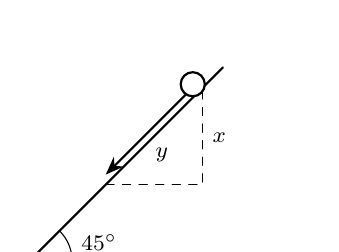
\begin{tikzpicture}[>=Stealth, scale=0.85, line cap=round, line join=round]
    \draw[thick] (0, 0) -- (4.2, 0);
    \draw[thick] (0, 0) -- (2.9, 2.9);
    \draw[thin] (0.65, 0) arc (0:45:0.65);
    \node[font=\footnotesize] at (1.05, 0.28) {$45^\circ$};
    % 石頭與位移箭頭
    \draw[thick, fill=white] (2.45, 2.65) circle (0.18);
    \draw[->, thick] (2.35, 2.50) -- (1.15, 1.30);
    \node[below right, font=\footnotesize] at (1.75, 1.85) {$y$};
    % 垂直高度 x 虛線直角三角形
    \draw[dashed] (1.15, 1.15) -- (2.6, 1.15) -- (2.6, 2.6);
    \node[right, font=\footnotesize] at (2.6, 1.85) {$x$};
  \end{tikzpicture}
  \end{center}
\end{enumerate}

\subsubsection*{乙、導函數}

當函數 $y=f(x)$ 到處都可微時，對應：
\[ x \longrightarrow f'(x) = \lim_{h\to 0}\dfrac{f(x+h)-f(x)}{h} \]
就成為一新函數，這新函數稱為 $y=f(x)$ 的\textbf{導函數}，通常以 $y'=f'(x)$ 或 $\dfrac{dy}{dx} = \dfrac{df(x)}{dx}$ 表之。

\begin{align*}
\text{〔例 7〕}\quad f(x)=cx+d \text{ 的導函數為 } y' &= c \\
\text{〔例 8〕}\quad f(x)=x^2 \text{ 的導函數為 } y' &= 2x \\
\text{〔例 9〕}\quad y=x^n \text{ 的導函數為 } y' &= nx^{n-1} \\
\text{〔例 10〕}\quad y=|x| \text{ 的導函數為 } y' &= \begin{cases} 1 & \text{當 } x>0 \\ -1 & \text{當 } x<0 \end{cases} \quad \text{當 } x=0 \text{ 時 } y' \text{ 無定義。} \\
\text{〔例 11〕}\quad y=\sqrt{x} \text{ 的導函數為 } y' &= \dfrac{1}{2\sqrt{x}}, \quad x>0
\end{align*}

由一個已知函數求出它的導函數的「運算」也叫做微分，下面我們來談一談微分這個新的運算和我們原來就熟悉函數間的運算如「加」，「減」，「乘」，「除」等的關係。

\begin{theorem}[微分運算的基本法則]\label{thm:b6s-app4-diff-rules}
令函數 $f(x), g(x)$ 為到處可微，則
\begin{enumerate}[label=(\roman*), leftmargin=2em]
  \item $\dfrac{d}{dx}(f(x)\pm g(x)) = \dfrac{df(x)}{dx} \pm \dfrac{dg(x)}{dx}$；
  \item $\dfrac{d}{dx}(f(x)g(x)) = \dfrac{df(x)}{dx}g(x) + f(x)\dfrac{dg(x)}{dx}$；
  \item $\dfrac{d}{dx}\left(\dfrac{f(x)}{g(x)}\right) = \dfrac{\dfrac{df(x)}{dx}g(x) - f(x)\dfrac{dg(x)}{dx}}{(g(x))^2}, \qquad (g(x)\ne 0)$；
  \item 若 $y=f(u), u=g(x)$ 即 $y=f(g(x))$ 為 $f, g$ 的合成函數，則
  \[ \dfrac{d}{dx}[f(g(x))] = \left[\dfrac{df(u)}{du}\right]\dfrac{dg(x)}{dx} \]
\end{enumerate}
\end{theorem}

\begin{proof}[【證明】]
(i), (ii) 直接由極限的性質而來，現在證明 (iii)：
\begin{align*}
\dfrac{d}{dx}\left(\dfrac{1}{g(x)}\right) &= \lim_{h\to 0}\dfrac{\dfrac{1}{g(x+h)} - \dfrac{1}{g(x)}}{h} = \lim_{h\to 0}\dfrac{-[g(x+h)-g(x)]}{h g(x+h)g(x)} \\
&= -\lim_{h\to 0}\dfrac{g(x+h)-g(x)}{h}\cdot\lim_{h\to 0}\dfrac{1}{g(x+h)g(x)} \\
&= -\dfrac{dg(x)}{dx}\cdot\dfrac{1}{[g(x)]^2}
\end{align*}
再由 (ii) 得
\begin{align*}
\dfrac{d}{dx}\left(\dfrac{f(x)}{g(x)}\right) &= \dfrac{df(x)}{dx}\cdot\dfrac{1}{g(x)} + f(x)\dfrac{d\left(\dfrac{1}{g(x)}\right)}{dx} \\
&= \dfrac{\dfrac{df(x)}{dx}g(x) - f(x)\dfrac{dg(x)}{dx}}{[g(x)]^2}
\end{align*}
(iv) 令 $k=g(x+h)-g(x)$，則 $g(x+h)=u+k$，而且當 $h\longrightarrow 0$ 時，$k\longrightarrow 0$，所以：
\begin{align*}
\dfrac{d}{dx}[f(g(x))] &= \lim_{h\to 0}\dfrac{f(g(x+h))-f(g(x))}{h} \\
&= \lim_{h\to 0}\left[\dfrac{f(u+k)-f(u)}{k}\cdot\dfrac{k}{h}\right] \\
&= \lim_{k\to 0}\dfrac{f(u+k)-f(u)}{k}\cdot\lim_{h\to 0}\dfrac{g(x+h)-g(x)}{h} \\
&= \dfrac{df(u)}{du}\cdot\dfrac{dg(x)}{dx}
\end{align*}
\end{proof}\hfill$\#$

上述諸式是計算函數不可或缺的工具，但這裡須注意公式 (iv) 並不是對一切函數都成立，這裡所說的條件並不完整，這裡的“證明”也不是一個完全的“證明”。這些精密的證明和條件我們不在這裡敘述，而留到大學正式微積分課作詳細證明。

\begin{example}\label{ex:b6s-app4-12}
$y=(2x+1)^2$ 可以看做 $y=u^2, u=2x+1$ 的合成函數，所以由 (iv) 得
\[ y' = \dfrac{dy}{du}\cdot\dfrac{du}{dx} = 2u \cdot 2 = 4(2x+1) \text{。}\hfill\# \]
\end{example}

\begin{example}\label{ex:b6s-app4-13}
$y=\sqrt{3x+1}, 3x+1>0$，試求 $y'$。
\end{example}

\paragraph{【解】}
令 $u=3x+1$，則 $y=\sqrt{u}$，故
\[ y' = \dfrac{d\sqrt{u}}{du}\cdot\dfrac{du}{dx} = \dfrac{1}{2\sqrt{u}}\cdot 3 = \dfrac{3}{2\sqrt{3x+1}} \text{。}\hfill\# \]

\subsubsection*{習題 2-B}\label{sec:b6s-ex-app4-2b}

試計算下列各式之導函數：
\begin{multicols}{2}
\begin{enumerate}[label=\arabic*., leftmargin=2em]
  \item $y = 3x^2$
  \item $y = 5x^3+4x^2+3x+2$
  \item $y = (3x^3+2x^2+x+1)^2$
  \item $y = (2x^2+1)(3x+2)$
  \item $y = \sqrt{2x-1}, (2x>1)$
  \item $y = \dfrac{1}{x^4}, (x\ne 0)$
  \item $y = \dfrac{1}{\sqrt{x+1}}, (x>-1)$
  \item $y = \sqrt{2x^2+3x+1}$
  \item $y = \left(\dfrac{2x+5}{3x+1}\right)^2$
  \item $y = (2x^2+4x-1)\sqrt{x^2+1}$
\end{enumerate}
\end{multicols}

\phantomsection
\subsection*{*§ 3\quad 幾個基本函數的微分}\label{subsec:b6s-app4-3}
\addcontentsline{toc}{subsection}{\texorpdfstring{*§ 3\quad 幾個基本函數的微分}{*§ 3 幾個基本函數的微分}}
\setcounter{lemma}{0}
\renewcommand{\thelemma}{3.\arabic{lemma}}
\setcounter{theorem}{1}
\renewcommand{\thetheorem}{3.\arabic{theorem}}

多項式，三角函數，和指數是我們常見而且應用最廣的幾種函數。上節例 9 和定理 2.1 已告訴我們多項式 $f(x)=a_0+a_1 x+\dots+a_n x^n$ 的導數為 $f'(x)=a_1+2a_2 x+\dots+n a_n x^{n-1}$。在這節裡我們來求三角函數和指數函數的導函數。

\subsubsection*{甲、三角函數的導函數}

我們先求 $y=\sin x$ 的導函數。要求 $y=\sin x$ 的導函數，必須利用下述的極限：

\begin{lemma}\label{lem:b6s-app4-sin-limit}
\[ \lim_{h\to 0}\dfrac{\sin h}{h} = 1 \]
\end{lemma}

\begin{figure}[H]
\centering
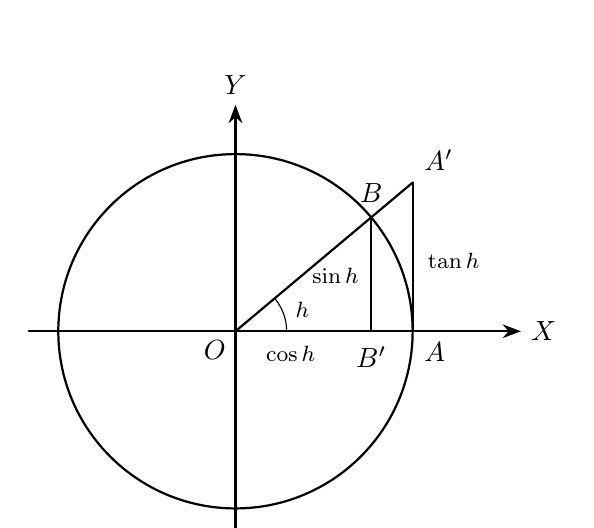
\begin{tikzpicture}[>=Stealth, scale=1.25, line cap=round, line join=round]
  \coordinate (O) at (0, 0);
  \draw[->, thick] (-2.1, 0) -- (2.9, 0) node[right] {$X$};
  \draw[->, thick] (0, -2.1) -- (0, 2.3) node[above] {$Y$};
  \node[below left] at (O) {$O$};

  % 完整單位圓 (與原書 p.192 一致，半徑 1.8，角度 40 度使 B' 與 A 清晰分離)
  \draw[thick] (O) circle (1.8);
  \coordinate (B) at (40:1.8);
  \coordinate (A) at (1.8, 0);
  \coordinate (Aprime) at (1.8, {1.8*tan(40)});
  \coordinate (Bprime) at ({1.8*cos(40)}, 0);

  \draw[thick] (O) -- (Aprime);
  \draw[thick] (A) -- (Aprime);
  \draw[thick] (B) -- (Bprime);

  \node[above=2pt] at (B) {$B$};
  \node[below right=1pt] at (A) {$A$};
  \node[above right=1pt] at (Aprime) {$A'$};
  \node[below=2pt] at (Bprime) {$B'$};

  \draw[thin] (0.52, 0) arc (0:40:0.52);
  \node[font=\footnotesize] at (0.68, 0.22) {$h$};
  \node[below=2pt, font=\footnotesize] at (0.56, 0) {$\cos h$};
  \node[left=1pt, font=\footnotesize] at ({1.8*cos(40)}, 0.56) {$\sin h$};
  \node[right=2pt, font=\footnotesize] at (1.8, 0.72) {$\tan h$};
\end{tikzpicture}
\caption{圖 3-1\quad $\lim_{h\to 0}\dfrac{\sin h}{h}=1$ 之單位圓幾何證明}
\label{fig:b6s-app4-sin-geom}
\end{figure}

\begin{proof}[【證明】]
參考圖 3-1，令圓 $O$ 為單位圓，則因為 $\triangle OBB' \subseteq \text{扇形 } OAB \subseteq \triangle OAA'$，而且
\begin{align*}
\triangle OBB' \text{ 的面積} &= \dfrac{1}{2}\sin h \cos h, \qquad \text{扇形 } OAB \text{ 的面積} = \dfrac{1}{2}\cdot 1 \cdot h, \\
\triangle OAA' \text{ 的面積} &= \dfrac{1}{2}\cdot 1 \cdot \tan h
\end{align*}
所以 $\sin h \cos h \le h \le \tan h$ 即 $\cos h \le \dfrac{\sin h}{h} \le \dfrac{1}{\cos h}$，所以當 $h\longrightarrow 0$ 時，$\cos h\longrightarrow 1, \dfrac{1}{\cos h}\longrightarrow 1$，故 $\lim_{h\to 0}\dfrac{\sin h}{h} = 1$。
\end{proof}\hfill$\#$

\begin{theorem}\label{thm:b6s-app4-deriv-sin}
\[ \dfrac{d}{dx}(\sin x) = \cos x \tag{I} \]
\end{theorem}

\begin{proof}[【證明】]
\begin{align*}
\dfrac{d}{dx}\sin x &= \lim_{h\to 0}\dfrac{\sin(x+h)-\sin x}{h} \\
&= \lim_{h\to 0}\dfrac{\sin x\cos h + \sin h\cos x - \sin x}{h} \\
&= \lim_{h\to 0}\left[\dfrac{\sin x(\cos h - 1)}{h} + \dfrac{\sin h}{h}\cos x\right] \\
&= \left(\lim_{h\to 0}\dfrac{\cos h - 1}{h}\right)\sin x + \left(\lim_{h\to 0}\dfrac{\sin h}{h}\right)\cos x = \cos x
\end{align*}
因為 $\lim_{h\to 0}\dfrac{\cos h - 1}{h} = \lim_{h\to 0}\dfrac{-2\sin^2\frac{h}{2}}{h} = \lim_{h\to 0}\left(-\sin\dfrac{h}{2}\right)\lim_{h\to 0}\dfrac{\sin\frac{h}{2}}{\frac{h}{2}} = 0$。
\end{proof}\hfill$\#$

應用 $\sin x$ 的導函數和上節所得的公式，我們已經可以求得其它三角函數的導函數：

\begin{theorem}\label{thm:b6s-app4-deriv-trig-other}
\begin{align*}
\dfrac{d}{dx}\cos x &= -\sin x \tag{II} \\
\dfrac{d}{dx}\tan x &= \sec^2 x \tag{III}
\end{align*}
\end{theorem}

\begin{proof}[【證明】]
(II) $\dfrac{d}{dx}\cos x = \dfrac{d}{dx}\sin\left(\dfrac{\pi}{2}+x\right) = \dfrac{d}{du}\sin u\cdot\dfrac{du}{dx}, \quad u=\dfrac{\pi}{2}+x$
\[ = \cos\left(\dfrac{\pi}{2}+x\right) = -\sin x \]
(III) $\dfrac{d}{dx}\tan x = \dfrac{d}{dx}\left(\dfrac{\sin x}{\cos x}\right) = \dfrac{\dfrac{d\sin x}{dx}\cos x - \sin x\dfrac{d\cos x}{dx}}{\cos^2 x} \quad (\text{定理 2.1, (iii)})$
\[ = \dfrac{\cos^2 x + \sin^2 x}{\cos^2 x} = \sec^2 x \quad (\text{(I), (II)}) \]
\end{proof}\hfill$\#$

\subsubsection*{乙、指數函數與對數函數的微分}

如果有家銀行的年利率是 $100\%$，存一元在該銀行一年後本利和為 $1+1=2$ 元。如果以複利計算每半年算一次，則一年後的本利率為 $\left(1+\frac{1}{2}\right)^2$ 元，每年算三次則為 $\left(1+\frac{1}{3}\right)^3$ 元，每年算 $n$ 次，則一年的本利和為 $\left(1+\frac{1}{n}\right)^n$ 元。當然 $n$ 增大時，其本利和也就增大，當 $n$ 無限的增大時，則其本利和是否會無限的增大？這就是說極限 $\lim_{n\to\infty}\left(1+\frac{1}{n}\right)^n$ 是否存在？答案是肯定的，這個極限在描寫自然現象上很重要，我們叫它尤拉數（Euler number）記為 $e$，以 $e$ 為底的對數就叫做\textbf{自然對數}。

\begin{theorem}\label{thm:b6s-app4-euler-e}
$e = \lim_{n\to\infty}\left(1+\dfrac{1}{n}\right)^n$ 存在。
\end{theorem}

\begin{proof}[【證明】]
a: $\left(1+\dfrac{1}{n}\right)^n$ 有上界，即有一 $c>0, \left(1+\dfrac{1}{n}\right)^n \le c$。因為由二項式定理知
\begin{align*}
\left(1+\dfrac{1}{n}\right)^n &= 1 + n\cdot\dfrac{1}{n} + \dfrac{n(n-1)}{2!}\left(\dfrac{1}{n}\right)^2 + \dots + \left(\dfrac{1}{n}\right)^n \\
&= 1 + 1 + \dfrac{1}{2!}\left(1-\dfrac{1}{n}\right) + \dots + \dfrac{1}{n!}\left(1-\dfrac{1}{n}\right)\dots\left(1-\dfrac{n-1}{n}\right) \\
&\le 1 + 1 + \dfrac{1}{2!} + \dots + \dfrac{1}{n!}
\end{align*}
但當 $n\ge 2$ 時，$n!\ge 2^{n-1}$，故 $\dfrac{1}{n!}\le\dfrac{1}{2^{n-1}}$，所以
\[ \left(1+\dfrac{1}{n}\right)^n \le 1 + 1 + \dfrac{1}{2} + \dfrac{1}{2^2} + \dots + \dfrac{1}{2^{n-1}} \le 3 \]
b: 數列 $a_n = \left(1+\dfrac{1}{n}\right)^n, n=1, 2, 3, \dots$ 為遞增數列，這由上面複利計算的例子很容易了解，$n+1>n$，所以 $\dfrac{1}{n}>\dfrac{1}{n+1}$，故 $\dfrac{k}{n}>\dfrac{k}{n+1}, k>0$，因此 $a_n \le a_{n+1}$。

由 a, b 和實數完備性（第二冊第三章 § 3-2），我們知道一遞增數列有上限時，它的極限 $e = \lim_{n\to\infty}\left(1+\dfrac{1}{n}\right)^n$ 存在。$e$ 的數值約等於 $2.71828182845904523536\dots$。
\end{proof}\hfill$\#$

令 $x=\dfrac{1}{h}$，則在 $h$ 從右邊（大於 0）趨近於 0 時，$x\longrightarrow\infty$。所以直觀上，我們有

\begin{theorem}\label{thm:b6s-app4-lim-h-e}
$\lim_{h\to 0}(1+h)^{\frac{1}{h}} = e$。
\end{theorem}

上面所敘述的並不是嚴格的證明，這些證明已經超過本書的範圍，在這裡不加以討論。以 $e$ 為底的對數我們叫它做自然對數，通常我們將 $\log_e x$ 記為 $\ln x$。

\setcounter{lemma}{5}
\begin{lemma}\label{lem:b6s-app4-e-limits}
\begin{enumerate}[label=(\roman*), leftmargin=2em]
  \item $\lim_{x\to 0}\dfrac{\ln(1+x)}{x} = 1$
  \item $\lim_{x\to 0}\dfrac{e^x-1}{x} = 1$
\end{enumerate}
\end{lemma}

\begin{proof}[【證明】]
(i) $\lim_{x\to 0}\dfrac{\ln(1+x)}{x} = \lim_{x\to 0}\ln(1+x)^{\frac{1}{x}} = \ln\lim_{x\to 0}(1+x)^{\frac{1}{x}} = \ln e = 1$。

(ii) 令 $e^x = 1+h$，則 $x=\ln(1+h)$，而且 $x\longrightarrow 0, h\longrightarrow 0$，故
\[ \lim_{x\to 0}\dfrac{e^x-1}{x} = \lim_{h\to 0}\dfrac{h}{\ln(1+h)} = \dfrac{1}{\lim_{h\to 0}\dfrac{\ln(1+h)}{h}} = 1 \]
\end{proof}\hfill$\#$

\setcounter{theorem}{6}
\begin{theorem}\label{thm:b6s-app4-deriv-exp-ln}
\begin{enumerate}[label=(\roman*), leftmargin=2em]
  \item $\dfrac{d}{dx}e^x = e^x$，
  \item $\dfrac{d}{dx}\ln x = \dfrac{1}{x}$
\end{enumerate}
\end{theorem}

\begin{proof}[【證明】]
(i) $\dfrac{d}{dx}e^x = \lim_{h\to 0}\dfrac{e^{x+h}-e^x}{h} = \lim_{h\to 0}\dfrac{e^x(e^h-1)}{h} = e^x\lim_{h\to 0}\dfrac{e^h-1}{h} = e^x$（引理 3.6(ii)）。

(ii) $\dfrac{d}{dx}\ln x = \lim_{h\to 0}\dfrac{\ln(x+h)-\ln x}{h} = \lim_{h\to 0}\dfrac{\ln\left(1+\frac{h}{x}\right)}{h}$。令 $t=\dfrac{h}{x}$，則 $h\longrightarrow 0$ 時，$t\longrightarrow 0$，
\[ \dfrac{d}{dx}\ln x = \lim_{h\to 0}\dfrac{1}{x}\dfrac{\ln\left(1+\frac{h}{x}\right)}{\frac{h}{x}} = \dfrac{1}{x}\lim_{t\to 0}\dfrac{\ln(1+t)}{t} = \dfrac{1}{x} \quad (\text{引理 3.6, (i)}) \]
\end{proof}\hfill$\#$

\begin{example}\label{ex:b6s-app4-14}
$a>0$，試求 $\dfrac{d}{dx} a^x$。
\end{example}

\paragraph{【解】}
$a^x = e^{x\ln a}$，故令 $u=x\ln a$，則 $\dfrac{d}{dx}a^x = \dfrac{d}{dx}e^{x\ln a} = \dfrac{d}{du}e^u \cdot \dfrac{d}{dx}(x\ln a) = (\ln a)e^u = (\ln a)e^{x\ln a} = (\ln a)a^x$。\hfill$\#$

\subsubsection*{丙、高階函數}

給一導函數 $f'(x)$，如果它的導函數存在，則稱為 $f(x)$ 的\textbf{第二階導函數}，並記之為 $f''(x)$，或寫成 $y'', \dfrac{d^2 y}{dx^2}, \dfrac{d^2}{dx^2}f(x)$。

\begin{example}\label{ex:b6s-app4-15}
求 $f(x)=3x^2+5x-2$ 的第二階導函數。
\end{example}

\paragraph{【解】}
因 $f'(x)=6x+5$，所以 $f''(x)=6$。\hfill$\#$

\begin{example}\label{ex:b6s-app4-16}
$f(x)=\sin x$ 的導函數為 $f'(x)=\cos x$，故其第二階導函數為 $f''(x)=-\sin x$。\hfill$\#$
\end{example}

依此類推，函數經過 $n$ 次微分之後，所得的函數叫做第 $n$ 階導函數，我們將它記為：$f^{(n)}(x), y^{(n)}, \dfrac{d^n}{dx^n}f(x)$ 或 $\dfrac{d^n y}{dx^n}$。

\begin{example}\label{ex:b6s-app4-17}
求 $y=x^n$ 的第 $n$ 階導函數。
\end{example}

\paragraph{【解】}
$\dfrac{dy}{dx} = nx^{n-1}, \dfrac{d^2 y}{dx^2} = n(n-1)x^{n-2}, \dots, \dfrac{d^n y}{dx^n} = n!$。\hfill$\#$

\subsubsection*{習題 3}\label{sec:b6s-ex-app4-3}

\begin{enumerate}[label=\Roman*., leftmargin=2em]
  \item 試求下列各函數的導函數：
  \begin{multicols}{2}
  \begin{enumerate}[label=\arabic*.]
    \item $x\sin x$
    \item $2x^2\sin x$
    \item $\sin x\cos x$
    \item $\dfrac{\sin x}{x}$
    \item $e^{-x}$
    \item $\dfrac{e^x}{x}$
    \item $x\ln x - x$
    \item $\log_{10} x$
    \item $e^x \ln x$
    \item $\ln(x^2+x+1)$
    \item $\ln\sqrt{1+x^2}$
    \item $\ln\sqrt{\dfrac{1+x}{1-x}}$
    \item $e^{-x}\sin(2x+1)$
    \item $e^x\sin^3 x$
    \item $a^{x^2}$
  \end{enumerate}
  \end{multicols}

  \item 試求習題 I 中各函數的第二階導函數。

  \item \textbf{簡諧運動}（如圖）：一質點沿一單位圓圓周作順時針等速圓周運動，即在時間 $t$ 時，其所掃過的角度為 $\theta(t)=\omega t$，$\omega$ 為常數。試問其在 $x$ 軸和 $y$ 軸上的投影的速率是多少？
  \begin{center}
  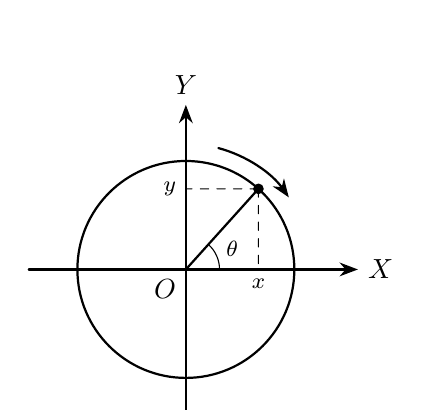
\begin{tikzpicture}[>=Stealth, scale=0.95, line cap=round, line join=round]
    \draw[->, thick] (-2.1, 0) -- (2.3, 0) node[right] {$X$};
    \draw[->, thick] (0, -2.0) -- (0, 2.2) node[above] {$Y$};
    \node[below left] at (0, 0) {$O$};
    \draw[thick] (0, 0) circle (1.45);
    \coordinate (P) at (48:1.45);
    \draw[thick] (0, 0) -- (P);
    \filldraw (P) circle (1.8pt);
    \draw[dashed] (P) -- ({1.45*cos(48)}, 0) node[below, font=\footnotesize] {$x$};
    \draw[dashed] (P) -- (0, {1.45*sin(48)}) node[left, font=\footnotesize] {$y$};
    \draw[thin] (0.45, 0) arc (0:48:0.45);
    \node[font=\footnotesize] at (0.62, 0.28) {$\theta$};
    % 順時針方向箭頭
    \draw[->, thick] (75:1.68) arc (75:35:1.68);
  \end{tikzpicture}
  \end{center}
\end{enumerate}

\phantomsection
\subsection*{§ 4\quad 函數圖形}\label{subsec:b6s-app4-4}
\addcontentsline{toc}{subsection}{\texorpdfstring{§ 4\quad 函數圖形}{§ 4 函數圖形}}
\setcounter{theorem}{0}
\renewcommand{\thetheorem}{4.\arabic{theorem}}

\subsubsection*{甲、切線方程式}

給一函數 $f(x)$，令 $y=f(x)$ 在平面上的圖形為 $C$，前面我們已經說明平均變率 $\dfrac{f(x)-f(x_0)}{x-x_0}$ 代表平面上，經過 $(x_0, f(x_0))$ 與 $(x, f(x))$ 的直線斜率（圖 4-1）。我們以 $L(x)$ 代表連接 $(x_0, f(x_0))$ 與 $(x, f(x))$ 的直線，則當 $x\longrightarrow x_0$ 時，直線 $L(x)$ 就趨近曲線 $C$ 在 $(x_0, f(x_0))$ 的切線 $L_0$。所以
\[ f'(x_0) = \lim_{x\to x_0}\dfrac{f(x)-f(x_0)}{x-x_0} \]
是 $C$ 在 $(x_0, f(x_0))$ 的切線的斜率，因此 $C$ 在 $(x_0, f(x_0))$ 的切線方程式為：
\[ y - f(x_0) = f'(x_0)(x - x_0) \]
有了這公式，一般曲線的切線方程式就很容易求了。

\begin{figure}[H]
\centering
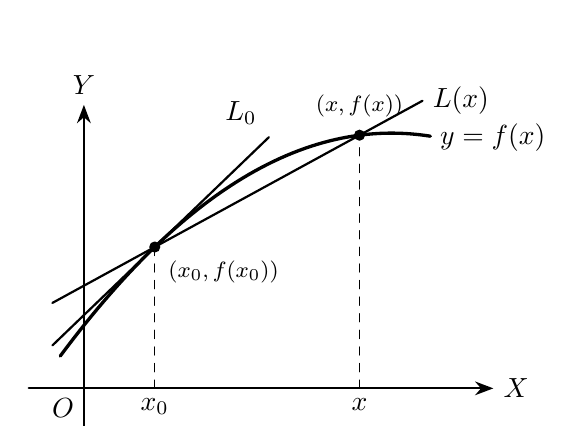
\begin{tikzpicture}[>=Stealth, scale=1.0, line cap=round, line join=round]
  \draw[->, thick] (-0.7, 0) -- (5.2, 0) node[right] {$X$};
  \draw[->, thick] (0, -0.6) -- (0, 3.6) node[above] {$Y$};
  \node[below left] at (0, 0) {$O$};

  % 凹向下曲線 y = f(x) = 0.8 + 1.25*x - 0.16*x^2 (與原書 p.200 一致，L0/L(x)/f(x) 絕不重疊)
  % f(0.9) = 1.7954, f'(0.9) = 0.962; f(3.5) = 3.215
  \draw[line width=1.2pt, domain=-0.3:4.4, samples=60] plot (\x, {0.8 + 1.25*\x - 0.16*\x*\x});
  \node[right] at (4.4, 3.18) {$y=f(x)$};

  \coordinate (P0) at (0.9, 1.795);
  \coordinate (P) at (3.5, 3.215);

  % 切線 L0: y = 1.795 + 0.962*(x - 0.9)
  \draw[thick] (-0.4, 0.545) -- (2.35, 3.190) node[above left=1pt] {$L_0$};
  % 割線 L(x): slope = (3.215 - 1.795)/2.6 = 0.546
  \draw[thick] (-0.4, 1.085) -- (4.3, 3.652) node[right] {$L(x)$};

  \filldraw (P0) circle (1.8pt) node[below right=2pt, font=\footnotesize] {$(x_0, f(x_0))$};
  \filldraw (P) circle (1.8pt) node[above=3pt, font=\footnotesize] {$(x, f(x))$};

  \draw[dashed] (0.9, 0) node[below] {$x_0$} -- (P0);
  \draw[dashed] (3.5, 0) node[below] {$x$} -- (P);
\end{tikzpicture}
\caption{圖 4-1\quad 割線極限與切線幾何關係}
\label{fig:b6s-app4-tangent-secant}
\end{figure}

\begin{example}\label{ex:b6s-app4-18}
求橢圓 $\dfrac{x^2}{a^2}+\dfrac{y^2}{b^2}=1$ 上經過 $(x_0, y_0)$ 的切線方程式。
\end{example}

\paragraph{【解】}
把 $y$ 看成 $x$ 的函數，令 $u=y^2$，則得 $u = b^2\left(1-\dfrac{x^2}{a^2}\right)$，
\[ \therefore \dfrac{du}{dx} = \dfrac{du}{dy}\dfrac{dy}{dx} = \dfrac{d}{dx}\left(b^2-\dfrac{b^2 x^2}{a^2}\right), \quad \text{即} \quad 2y\dfrac{dy}{dx} = -\dfrac{2b^2 x}{a^2} \implies \left.\dfrac{dy}{dx}\right|_0 = -\dfrac{b^2 x_0}{a^2 y_0} \]

\begin{figure}[H]
\centering
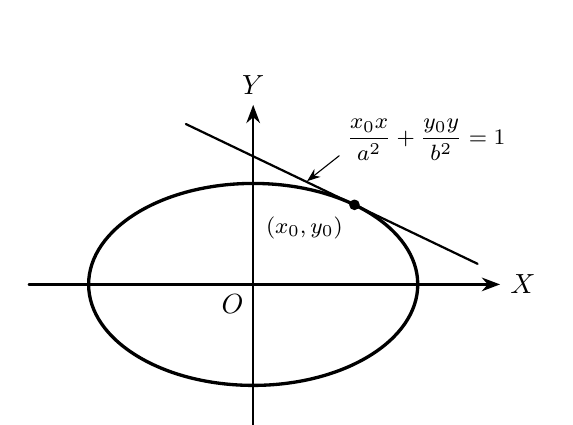
\begin{tikzpicture}[>=Stealth, scale=0.95, line cap=round, line join=round]
  \draw[->, thick] (-3.0, 0) -- (3.3, 0) node[right] {$X$};
  \draw[->, thick] (0, -2.0) -- (0, 2.4) node[above] {$Y$};
  \node[below left] at (0, 0) {$O$};

  % 橢圓 (a=2.2, b=1.35) 與點 (x0, y0) = (2.2*cos 52, 1.35*sin 52) = (1.354, 1.064)
  \draw[line width=1.2pt] (0, 0) ellipse (2.2 and 1.35);
  \coordinate (P0) at (1.354, 1.064);
  % 切線: (1.354/4.84)x + (1.064/1.8225)y = 1 => 0.2798x + 0.5838y = 1 => slope = -0.479
  \draw[thick] (-0.9, 2.144) -- (3.0, 0.275);
  \filldraw (P0) circle (1.8pt) node[below left=1pt, font=\footnotesize] {$(x_0, y_0)$};
  \draw[->, thin] (1.15, 1.72) -- (0.72, 1.38);
  \node[above right, font=\footnotesize] at (1.12, 1.52) {$\dfrac{x_0 x}{a^2}+\dfrac{y_0 y}{b^2}=1$};
\end{tikzpicture}
\caption{圖 4-2\quad 橢圓上一點 $(x_0, y_0)$ 之切線}
\label{fig:b6s-app4-ellipse-tangent}
\end{figure}

所以切線方程式為 $y-y_0 = -\dfrac{b^2 x_0}{a^2 y_0}(x-x_0)$，化簡之得：
\[ \dfrac{x_0 x}{a^2} + \dfrac{y_0 y}{b^2} = 1 \text{。}\hfill\# \]

\begin{example}\label{ex:b6s-app4-19}
求 $y=\sin x$ 在 $(0,0)$ 的切線方程式。
\end{example}

\paragraph{【解】}
因為 $f'(0)=\cos 0 = 1$，所以在 $(0,0)$ 的切線方程式為 $y=x$。\hfill$\#$

\begin{figure}[H]
\centering
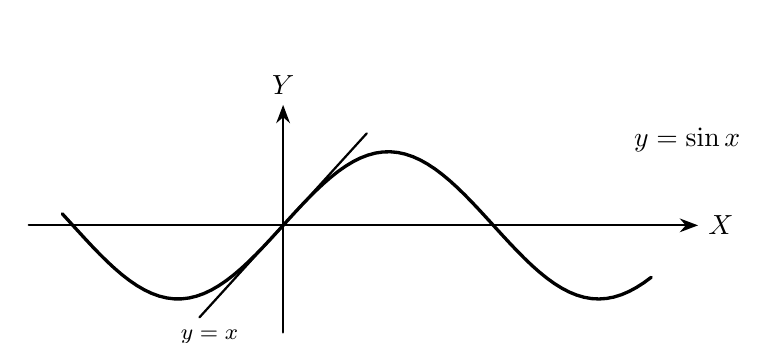
\begin{tikzpicture}[>=Stealth, scale=0.85, line cap=round, line join=round]
  \draw[->, thick] (-3.8, 0) -- (6.2, 0) node[right] {$X$};
  \draw[->, thick] (0, -1.6) -- (0, 1.8) node[above] {$Y$};
  % 正弦曲線 y = sin(x)
  \draw[line width=1.2pt, domain=-3.3:5.5, samples=80] plot (\x, {1.1*sin(\x r)});
  \node[above right] at (5.1, 0.95) {$y=\sin x$};
  % 原點切線 y = x (斜率 1.1 因縱軸放大 1.1 倍以相切)
  \draw[thick] (-1.25, -1.375) -- (1.25, 1.375);
  \node[below, font=\footnotesize] at (-1.1, -1.42) {$y=x$};
\end{tikzpicture}
\caption{圖 4-3\quad $y=\sin x$ 在原點之切線 $y=x$}
\label{fig:b6s-app4-sin-tangent}
\end{figure}

\begin{example}\label{ex:b6s-app4-20}
求 $y=e^x$ 在 $(0,1)$ 的切線方程式。
\end{example}

\paragraph{【解】}
因為 $f'(0)=1$，所以在 $(0,1)$ 的切線方程式為 $y-1=x$，即 $y=x+1$。\hfill$\#$

\subsubsection*{作業 4}
試求下列各曲線在 $(x_0, y_0)$ 的切線方程式：
\begin{enumerate}[label=(\roman*), leftmargin=2em]
  \item 拋物線 $y^2 = 4ax$
  \item 雙曲線 $\dfrac{x^2}{a^2} - \dfrac{y^2}{b^2} = 1$
  \item 雙曲線 $xy = a$
  \item 對數曲線 $y = \ln x$
\end{enumerate}

\subsubsection*{乙、極大，極小}

如圖 4-4 所示，我們知道（見本冊第二章第四節），如果 $f(x_0)$ 是極小值則在它的附近，所有的 $f(x)$ 都大於或等於 $f(x_0)$，這是說存在有一 $h_0>0$，使所有的 $x\in[x_0-h_0, x_0+h_0], f(x)\ge f(x_0)$。所以當 $|h|<h_0$ 時，$f(x_0+h)\ge f(x_0)$，因此當 $h<0$，而且 $|h|<|h_0|$ 時，

\begin{figure}[H]
\centering
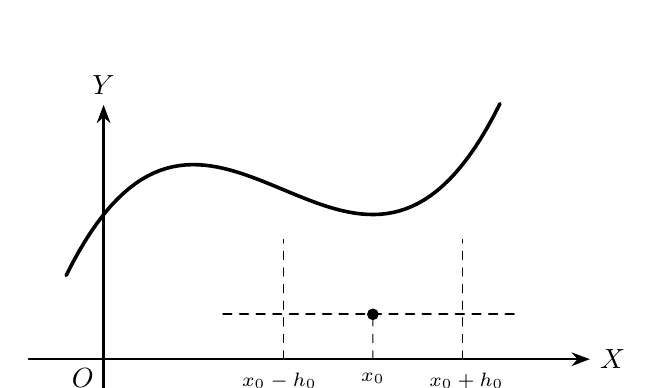
\begin{tikzpicture}[>=Stealth, scale=0.95, line cap=round, line join=round]
  \draw[->, thick] (-1.0, 0) -- (6.5, 0) node[right] {$X$};
  \draw[->, thick] (0, -0.5) -- (0, 3.4) node[above] {$Y$};
  \node[below left] at (0, 0) {$O$};

  % 顯式三次函數：極大於 x=1.2 (y=2.6), 極小於 x=3.6 (y=0.6)
  % f'(x) = 0.29*(x-1.2)*(x-3.6) = 0.29*(x^2 - 4.8x + 4.32)
  % f(x) = 0.0967*x^3 - 0.696*x^2 + 1.2528*x + 1.933 -> check: f(1.2)=2.60, f(3.6)=0.60, f(2.4)=1.60, f(4.8)=1.60
  \draw[line width=1.3pt, domain=-0.5:5.3, samples=70]
    plot (\x, {0.0967*\x*\x*\x - 0.696*\x*\x + 1.2528*\x + 1.933});

  \coordinate (X0) at (3.6, 0.60);
  \draw[dashed] (2.4, 0) -- (2.4, 1.60);
  \draw[dashed] (3.6, 0) -- (X0);
  \draw[dashed] (4.8, 0) -- (4.8, 1.60);

  \node[below, font=\scriptsize] at (2.35, -0.05) {$x_0-h_0$};
  \node[below, font=\scriptsize] at (3.60, -0.05) {$x_0$};
  \node[below, font=\scriptsize] at (4.85, -0.05) {$x_0+h_0$};

  \filldraw (X0) circle (2pt);
  \draw[thick, dashed] (1.6, 0.60) -- (5.5, 0.60); % 水平切線
\end{tikzpicture}
\caption{圖 4-4\quad 局部極值點之水平切線特徵}
\label{fig:b6s-app4-extrema-geom}
\end{figure}

\[ \dfrac{f(x_0+h)-f(x_0)}{h} \le 0, \quad \text{即} \quad \lim_{h\to 0^-}\dfrac{f(x_0+h)-f(x_0)}{h} \le 0 \tag{I} \]
同理，當 $h>0$，而且 $|h|<h_0$ 時，
\[ \dfrac{f(x_0+h)-f(x_0)}{h} \ge 0, \quad \text{即} \quad \lim_{h\to 0^+}\dfrac{f(x_0+h)-f(x_0)}{h} \ge 0 \tag{II} \]
如果 $f(x)$ 在 $x=x_0$ 時可微，則 $\lim_{h\to 0}\dfrac{f(x_0+h)-f(x_0)}{h} = f'(x_0)$ 存在，但由 (I) 知 $f'(x_0)\le 0$，由 (II) 知 $f'(x_0)\ge 0$，所以
\[ f'(x_0) = 0 \]

\begin{theorem}\label{thm:b6s-app4-extrema-zero}
如果函數 $f(x)$ 在 $x=x_0$ 時可微，而且 $f(x_0)$ 為極小值時，則 $f'(x_0) = 0$。
\end{theorem}

同理可證：

\begin{theorem}\label{thm:b6s-app4-extrema-max}
如果函數 $f(x)$ 在 $x=x_0$ 時可微，而且 $f(x_0)$ 為極大值時，則 $f'(x_0) = 0$。
\end{theorem}

\subsubsection*{作業 5}
試證定理 4.2。

我們再觀察圖 4-4，當 $f(x_0)$ 為極小值時的情形，因為在 $x=x_0$ 附近的 $f(x)$ 都不小於 $f(x_0)$，所以在 $x=x_0$ 左邊的 $f(x)$ 由 $\ge f(x_0)$ 而漸漸等於 $f(x_0)$，所以越來越小，這種情形叫做下降，用符號表示，就是說，如果在區間 $[a, b]$ 內，對於 $x, y\in[a, b], x\le y$ 時，$f(x)\ge f(y)$，則稱 $f(x)$ 在 $[a, b]$ 內下降。如果對於 $x, y\in[a, b], x\le y \implies f(x)\le f(y)$，稱 $f(x)$ 在 $[a, b]$ 上昇。

只要觀察圖形，我們就會知道下降和上昇這兩個名詞是完全由自然現象定義出來的。而且我們很容易觀察出來，當 $f(x_0)$ 為極小值時，在 $x=x_0$ 的左邊必有一個區域 $f(x)$ 下降，在 $x=x_0$ 的右邊，有一區域 $f(x)$ 上昇。

現在我們用微分法來研討函數的下降與上昇的問題。假設 $a<x_0<b$，函數 $f(x)$ 在區間 $[a, b]$ 內下降（如圖 4-5），則當 $h>0, x_0+h<b$ 時，$f(x_0)-f(x_0+h) \ge 0$，所以 $\dfrac{f(x_0+h)-f(x_0)}{h} \le 0$；當 $h<0, a<x_0+h<x_0$ 時，$f(x_0+h)-f(x_0) \ge 0$，所以 $\dfrac{f(x_0+h)-f(x_0)}{h} \le 0$（因 $h<0$）。如果 $f(x)$ 在 $x=x_0$ 可微，則 $f'(x_0)$ 存在，因此得 $f'(x_0) = \lim_{h\to 0}\dfrac{f(x_0+h)-f(x_0)}{h} \le 0$。因此我們得到下述的性質：

\begin{figure}[H]
\centering
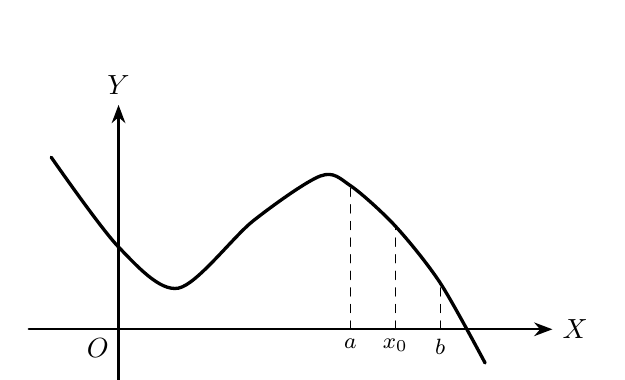
\begin{tikzpicture}[>=Stealth, scale=0.95, line cap=round, line join=round]
  \draw[->, thick] (-1.2, 0) -- (5.8, 0) node[right] {$X$};
  \draw[->, thick] (0, -0.8) -- (0, 3.0) node[above] {$Y$};
  \node[below left] at (0, 0) {$O$};
  % 與原書 p.204 一致：局部極小在 x=0.8，極大在 x=2.7，[a, b] 在下降段 [3.0, 4.4]
  \draw[line width=1.2pt, smooth] plot coordinates {
    (-0.9, 2.3) (0.0, 1.1) (0.8, 0.55) (1.8, 1.45) (2.7, 2.05) (3.1, 1.92) (3.7, 1.38) (4.3, 0.62) (4.9, -0.45)
  };
  \draw[dashed] (3.1, 0) node[below, font=\footnotesize] {$a$} -- (3.1, 1.92);
  \draw[dashed] (3.7, 0) node[below, font=\footnotesize] {$x_0$} -- (3.7, 1.38);
  \draw[dashed] (4.3, 0) node[below, font=\footnotesize] {$b$} -- (4.3, 0.62);
\end{tikzpicture}
\caption{圖 4-5\quad 函數於區間 $[a, b]$ 內下降之幾何示意}
\label{fig:b6s-app4-decreasing}
\end{figure}

\begin{theorem}\label{thm:b6s-app4-monotonicity}
如果 $f(x)$ 在區間 $[a, b]$ 內可微而且下降，則對於 $a<x_0<b, f'(x_0) \le 0$。
\end{theorem}

同理可證：

\begin{theorem}\label{thm:b6s-app4-monotonicity-inc}
如果 $f(x)$ 在區間 $[a, b]$ 內可微而且上昇，則對於 $a<x_0<b, f'(x_0) \ge 0$。
\end{theorem}

\subsubsection*{作業 6}
試證定理 4.4。

一個函數的極大值和極小值，我們通稱為極值。由定理 4.1--4.4，我們已經可以判斷可微函數的極值問題。

\begin{example}\label{ex:b6s-app4-21}
求 $y=ax^2+bx+c$ 的極值，$a\ne 0$。
\end{example}

\paragraph{【解】}
若 $f(x_0)$ 為 $y$ 的極值，則 $f'(x_0)=0$，即 $2ax_0+b=0$，所以 $x_0 = -\dfrac{b}{2a}$。
\begin{enumerate}[label=\roman*), leftmargin=2em]
  \item 如果 $a>0$，則當 $x<\dfrac{-b}{2a}$ 時，$f'(x)=(2ax+b)<2a\left(\dfrac{-b}{2a}\right)+b=0$；當 $x>\dfrac{-b}{2a}$ 時，$f'(x)>0$，故 $f(x_0)$ 為極小值。
  \item 同理 $a<0$ 時，$f(x_0)$ 為極大值。（試證之）\hfill$\#$
\end{enumerate}

\begin{example}\label{ex:b6s-app4-22}
求 $y=\sin x$ 的極值。
\end{example}

\paragraph{【解】}
$y'=\cos x$，所以 $y$ 的極值在 $x = \dfrac{\pi}{2}+k\pi, k=0, 1, 2, \dots$。\hfill$\#$

\subsubsection*{作業 7}
試證當 $k$ 為偶數時，$\sin\left(\dfrac{\pi}{2}+k\pi\right)$ 為極大值，當 $k$ 為奇數時 $\sin\left(\dfrac{\pi}{2}+k\pi\right)$ 為極小值\phantomsection\label{note:b6s-app4-p205-sin}\footnote{【原書校訂】：原書此處誤印為「$\sin k\pi$」，對照例 22 極值點應為「$\sin\left(\dfrac{\pi}{2}+k\pi\right)$」，茲予校訂。}。

\subsubsection*{作業 8}
求下列各函數的極值：
\begin{multicols}{2}
\begin{enumerate}[label=\roman*)]
  \item $x^5 - 5x^4 + 5x^3$
  \item $x + \dfrac{1}{x}$
  \item $\dfrac{1}{\cos 2\theta}, \left(-\frac{\pi}{4}<\theta<\frac{\pi}{4}\right)$
  \item $\sin x + \sin 2x$
\end{enumerate}
\end{multicols}

\phantomsection
\subsection*{§ 5\quad 近似值}\label{subsec:b6s-app4-5}
\addcontentsline{toc}{subsection}{\texorpdfstring{§ 5\quad 近似值}{§ 5 近似值}}
\setcounter{theorem}{0}
\renewcommand{\thetheorem}{5.\arabic{theorem}}

微分法一個很實際的應用是函數近似值的計算，下面我們介紹泰勒（Taylor）公式和牛頓式的求根法。

\subsubsection*{甲、均值定理與泰勒公式}

假設圖 5-1 是函數 $y=f(x)$ 從 $x=a$ 到 $x=b$ 間的圖形，$P=(a, f(a)), Q=(b, f(b))$，而且 $y=f(x)$ 在這區間內每一點都可微，以平行於線段 $PQ$ 的直線 $L$ 向下或向上移動，則一定有一個位置 $x=c$，使 $L$ 成為其圖形在 $(c, f(c))$ 的切線，在這一點 $f'(c) = \dfrac{f(b)-f(a)}{b-a}$。我們得到了：

\begin{figure}[H]
\centering
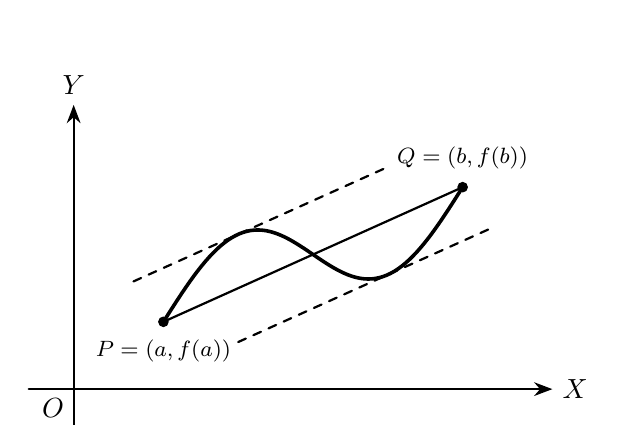
\begin{tikzpicture}[>=Stealth, scale=0.95, line cap=round, line join=round]
  \draw[->, thick] (-0.6, 0) -- (6.4, 0) node[right] {$X$};
  \draw[->, thick] (0, -0.6) -- (0, 3.8) node[above] {$Y$};
  \node[below left] at (0, 0) {$O$};

  % 與原書 p.205 圖 5-1 一致：S 型曲線精確通過 P(1.2, 0.9) 與 Q(5.2, 2.7)
  % 直線 PQ 斜率 m = (2.7 - 0.9)/4.0 = 0.45: L(x) = 0.9 + 0.45*(x - 1.2)
  % 曲線 y(x) = 0.9 + 0.45*(x - 1.2) + 0.72*sin((x - 1.2)*90) -> 在 x=1.2 時 y=0.9 (P), 在 x=5.2 時 y=2.7 (Q)
  % 極值點 (y'(x)=0.45): x1 = 2.2 (offset +0.72), x2 = 4.2 (offset -0.72)
  \coordinate (P) at (1.2, 0.9);
  \coordinate (Q) at (5.2, 2.7);

  \draw[line width=1.3pt, domain=1.2:5.2, samples=80]
    plot (\x, {0.9 + 0.45*(\x - 1.2) + 0.72*sin((\x - 1.2)*90)});

  % 弦 PQ
  \draw[thick] (P) -- (Q);
  \filldraw (P) circle (1.8pt) node[below=3pt, font=\footnotesize] {$P=(a, f(a))$};
  \filldraw (Q) circle (1.8pt) node[above=3pt, font=\footnotesize] {$Q=(b, f(b))$};

  % 上下兩條與 PQ 平行的切線 (精確相切於 x=2.2 與 x=4.2)
  \draw[thick, dashed] (0.8, {0.9 + 0.45*(-0.4) + 0.72}) -- (4.2, {0.9 + 0.45*(3.0) + 0.72});
  \draw[thick, dashed] (2.2, {0.9 + 0.45*(1.0) - 0.72}) -- (5.6, {0.9 + 0.45*(4.4) - 0.72});
\end{tikzpicture}
\caption{圖 5-1\quad 微分均值定理之幾何意義}
\label{fig:b6s-app4-mvt}
\end{figure}

\begin{theorem}[均值定理]\label{thm:b6s-app4-mvt}
若 $f(x)$ 在 $a\le x\le b$ 間連續而且 $f(x)$ 在 $a<x<b$ 內可微，則存在一個 $c, a<c<b$ 使得
\[ f'(c) = \dfrac{f(b)-f(a)}{b-a} \]
\end{theorem}

由此定理，我們可以證明下面的重要公式：

\begin{theorem}[泰勒公式]\label{thm:b6s-app4-taylor}
設函數 $f(x)$ 在 $a_0\le x\le b_0$ 上有連續的導函數 $f'(x)$, $f''(x)$, $\dots$, $f^{(n)}(x)$，而且在 $a_0<x<b_0$ 內 $f^{(n+1)}(x)$ 存在，則對於任意的 $a_0\le a<b\le b_0$，存在一點 $c, a<c<b$ 使得
\[ f(b) = f(a) + \dfrac{f'(a)}{1!}(b-a) + \dfrac{f''(a)}{2!}(b-a)^2 + \dots + \dfrac{f^{(n)}(a)}{n!}(b-a)^n + R_n \]
其中 $R_n = \dfrac{f^{(n+1)}(c)}{(n+1)!}(b-a)^{n+1}$ 稱為餘式。
\end{theorem}

\begin{proof}[【證明】]
對於 $a\le x\le b$，我們定義
\begin{align*}
F(x) = f(x) - \biggl[ &f(a) + \dfrac{f'(a)}{1!}(x-a) + \dfrac{f''(a)}{2!}(x-a)^2 + \dots \\
&+ \dfrac{f^{(n)}(a)}{n!}(x-a)^n + k(x-a)^{n+1} \biggr]
\end{align*}
顯然 $F(a)=0$。如果我們選取
\begin{equation}
k = \dfrac{f(b) - \left[ f(a) + \dfrac{f'(a)}{1!}(b-a) + \dots + \dfrac{f^{(n)}(a)}{n!}(b-a)^n \right]}{(b-a)^{n+1}} \tag{I} \label{eq:b6s-app4-taylor-k}
\end{equation}
則 $F(b)=0$，所以由均值定理必有一 $c_1, a<c_1<b$，使得 $F'(c_1)=0$。但
\[ F'(x) = f'(x) - \left[ f'(a) + f''(a)(x-a) + \dots + \dfrac{f^{(n)}(a)}{(n-1)!}(x-a)^{n-1} + (n+1)k(x-a)^n \right] \]
所以 $F'(a)=0$，再由均值定理，知道必有 $c_2, a<c_2<c_1$ 使 $F''(c_2)=0$。這樣繼續下去，我們得到 $a<c_{n+1}<c_n<\dots<c_2<c_1<b$，使得 $F^{(i)}(c_i)=0, i=1, 2, \dots, n+1$。到第 $n+1$ 次時
\[ F^{(n+1)}(x) = f^{(n+1)}(x) - (n+1)!k \]
令 $c=c_{n+1}$，得 $k = \dfrac{f^{(n+1)}(c)}{(n+1)!}$，代入 (I) 式可得泰勒公式。
\end{proof}\hfill$\#$

泰勒公式的證明，以現階段而言似乎難了一些，我們只要能應用就好了。以 $b=x$ 代入，我們可以由各階導函數 $f(x), f'(x), \dots, f^{(n)}(x)$ 在 $x=a$ 的值，來估計 $f(x)$ 的值：
\[ f(x) = f(a) + \dfrac{f'(a)}{1!}(x-a) + \dfrac{f''(a)}{2!}(x-a)^2 + \dots + \dfrac{f^{(n)}(a)}{n!}(x-a)^n + R_n \]
其中 $R_n = \dfrac{f^{(n+1)}(c)}{(n+1)!}(x-a)^{n+1}, |a-c|<|x-a|$，為餘式。在泰勒公式中，如果 $n$ 只取到 1 時，就是均值定理，所以均值定理就是原函數一次逼近的近似值：
\[ f(x) = f(a) + (x-a)f'(c), \qquad a<c<x \]

\setcounter{example}{23}
\begin{example}\label{ex:b6s-app4-24}
求 $y=\sin x$ 在 $x=0$ 附近的泰勒公式。
\end{example}

\paragraph{【解】}
$\left.y\right|_0 = 0, \left.y'\right|_0 = 1, \left.y''\right|_0 = 0, \left.y^{(3)}\right|_0 = -1, \dots, \left.y^{(2k)}\right|_0 = 0, \left.y^{(2k+1)}\right|_0 = (-1)^k, \dots$，故
\[ \sin x = x - \dfrac{x^3}{3!} + \dfrac{x^5}{5!} - \dots + (-1)^k\dfrac{x^{2k+1}}{(2k+1)!} + \dots + R_n \]
其中 $R_n = \left.\dfrac{d^{n+1}}{dx^{n+1}}\sin x\right|_c \dfrac{x^{n+1}}{(n+1)!}, \quad 0<c<x$。\hfill$\#$

\subsubsection*{乙、牛頓式求根法}

如圖 5-2，設 $y=f(x)$ 有一個根 $\bar{x}$，則 $y=f(x)$ 的圖形與 $x$ 軸有一個交點 $(\bar{x}, 0)$。如果 $x_0$ 相當接近於 $\bar{x}$，則 $y=f(x)$ 在 $(x_0, f(x_0))$ 的切線與 $x$ 軸交點的 $x$ 座標 $x_1$ 會比 $x_0$ 更加接近於 $\bar{x}$，但在 $(x_0, f(x_0))$ 的切線方程式是 $y-f(x_0) = f'(x_0)(x-x_0)$，所以與 $x$ 軸交點的 $x$ 座標為
\[ x_1 = x_0 - \dfrac{f(x_0)}{f'(x_0)} \]
同理 $y=f(x)$ 在 $(x_1, f(x_1))$ 的切線與 $x$ 軸交點的 $x$ 座標 $x_2$ 也比 $x_1$ 更靠近 $\bar{x}$，而且 $x_2 = x_1 - \dfrac{f(x_1)}{f'(x_1)}$。這步驟可以一直做下去，就是說，求得 $x_n$ 後再計算 $x_{n+1}$ 的公式為：
\begin{equation}
x_{n+1} = x_n - \dfrac{f(x_n)}{f'(x_n)} \label{eq:b6s-app4-newton}
\end{equation}
就可得到一數列 $x_0, x_1, x_2, \dots$ 使 $\lim_{n\to\infty} x_n = \bar{x}$。這就是\textbf{牛頓式的求根法}。

\begin{figure}[H]
\centering
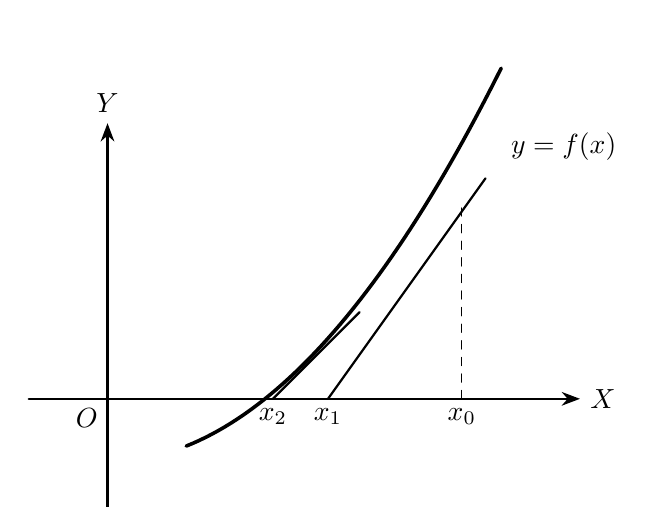
\begin{tikzpicture}[>=Stealth, scale=1.0, line cap=round, line join=round]
  \draw[->, thick] (-1, 0) -- (6.0, 0) node[right] {$X$};
  \draw[->, thick] (0, -1.5) -- (0, 3.5) node[above] {$Y$};
  \node[below left] at (0, 0) {$O$};

  % 曲線 y = f(x)
  \draw[line width=1.3pt, domain=1.0:5.0, samples=50] plot (\x, {0.2*(\x-2)^2 + 0.8*(\x-2)});
  \node[right] at (5.0, 3.2) {$y=f(x)$};

  % 切線從 x0
  \coordinate (P0) at (4.5, 2.5);
  \draw[thick] (2.8, 0) -- (4.8, 2.8);
  \draw[dashed] (4.5, 0) node[below] {$x_0$} -- (P0);
  \node[below] at (2.8, 0) {$x_1$};

  \coordinate (P1) at (2.8, 0.7);
  \draw[thick] (2.1, 0) -- (3.2, 1.1);
  \node[below] at (2.1, 0) {$x_2$};
\end{tikzpicture}
\caption{圖 5-2\quad 牛頓切線法逼近實根幾何模型}
\label{fig:b6s-app4-newton-geom}
\end{figure}

\begin{example}\label{ex:b6s-app4-25}
試求 $f(x)=x^3+x^2+x-2$ 的實根的近似值。
\end{example}

\paragraph{【解】}
因為 $f(0)=-2, f(1)=1$，所以在 0 與 1 間有它的實根，現在 $f'(x)=3x^2+2x+1$。令 $x_0=1$，則
\begin{align*}
x_1 &= 1 - \dfrac{f(1)}{f'(1)} = 1 - \dfrac{1}{6} \doteq 0.833 \\
x_2 &= 0.8333 - \dfrac{f(0.8333)}{f'(0.8333)} \doteq 0.8109
\end{align*}
所以 0.81 為二位正確數值（為甚麼？）。\hfill$\#$

牛頓法求根有一個好處，就是求得 $x_0$ 再由 $x_0$ 求 $x_1$ 的公式與由 $x_n$ 求 $x_{n+1}$ 的公式完全相同。所以可以把它放在電子計算機內操作，因此它在實用上很重要。

\subsubsection*{習題 5}\label{sec:b6s-ex-app4-5}

\begin{enumerate}[label=\arabic*., leftmargin=2em]
  \item 對於多項式，這裏所說的泰勒展開式和第二章所說的泰勒展開式是否相同？試說明之。
  \item 求下列各函數在 $x=a$ 的泰勒展開式：
  \begin{multicols}{2}
  \begin{enumerate}[label=\roman*)]
    \item $\cos x, a=0$
    \item $x^4+6x^3-3x^2+x-1, a=1$
    \item $e^x, a=0$
    \item $\sqrt{x+1}, a=3$
  \end{enumerate}
  \end{multicols}
  \item 求 $\sqrt{2}$ 到小數點以下三位正確數目（由牛頓求根法）。
  \item 求下列各方程式的實根近似值到小數點以下二位正確數值：
  \begin{enumerate}[label=\roman*)]
    \item $x^3-12x+1=0$，實根在 0 與 1 之間
    \item $x^3-3x^2+2=0$，實根在 2 與 3 之間
    \item $x^3+3x-7=0$，實根在 1 與 2 之間
  \end{enumerate}
\end{enumerate}

\phantomsection
\subsection*{§ 6\quad 導數與面積}\label{subsec:b6s-app4-6}
\addcontentsline{toc}{subsection}{\texorpdfstring{§ 6\quad 導數與面積}{§ 6 導數與面積}}
\setcounter{theorem}{0}
\renewcommand{\thetheorem}{6.\arabic{theorem}}

到現在程度，我們所能計算的平面圖形的面積，只限於如正方形、矩形、平行四邊形等直線形和圓形與扇形等幾個特殊平面圖形的面積。在計算圓形和扇形時，我們是用逼近它們的直線形的面積的極限而求出它們的面積的，這個方法可以應用於一般平面圖形的面積的計算。

\begin{example}\label{ex:b6s-app4-26}
如圖 6-1，求 $y=x^2$ 與 $x$ 軸從 $x=0$ 到 $x=a$ 所包圍（斜線部份）的面積。
\end{example}

\begin{figure}[H]
\centering
\begin{subfigure}[b]{0.45\textwidth}
\centering
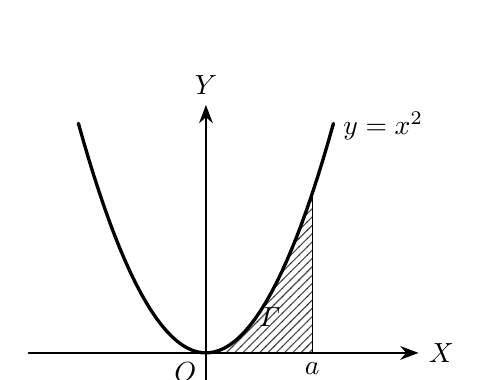
\begin{tikzpicture}[>=Stealth, scale=0.9, line cap=round, line join=round]
  \draw[->, thick] (-2.5, 0) -- (3.0, 0) node[right] {$X$};
  \draw[->, thick] (0, -0.5) -- (0, 3.5) node[above] {$Y$};
  \node[below left] at (0, 0) {$O$};

  \draw[line width=1.2pt, domain=-1.8:1.8, samples=50] plot (\x, {\x*\x});
  \node[right] at (1.8, 3.2) {$y=x^2$};

  % 斜線面積 (0 到 a, 取 a=1.5)
  \fill[pattern=north east lines, opacity=0.7] (0, 0) -- plot[domain=0:1.5] (\x, {\x*\x}) -- (1.5, 0) -- cycle;
  \draw (1.5, 0) node[below] {$a$} -- (1.5, 2.25);
  \node at (0.9, 0.5) {$\varGamma$};
\end{tikzpicture}
\caption{圖 6-1(a)}
\end{subfigure}
\begin{subfigure}[b]{0.45\textwidth}
\centering
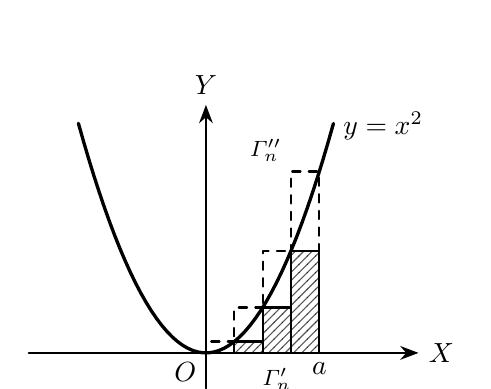
\begin{tikzpicture}[>=Stealth, scale=0.9, line cap=round, line join=round]
  \draw[->, thick] (-2.5, 0) -- (3.0, 0) node[right] {$X$};
  \draw[->, thick] (0, -0.5) -- (0, 3.5) node[above] {$Y$};
  \node[below left] at (0, 0) {$O$};

  \draw[line width=1.2pt, domain=-1.8:1.8, samples=50] plot (\x, {\x*\x});
  \node[right] at (1.8, 3.2) {$y=x^2$};

  % 上下階梯形矩形逼近 (n=4, a=1.6, 與原書 p.210 圖 6-1(b) 一致)
  \foreach \i in {1, 2, 3} {
    \fill[pattern=north east lines, opacity=0.65] ({\i*0.4}, 0) rectangle ({(\i+1)*0.4}, {(\i*0.4)^2});
    \draw[thick] ({\i*0.4}, 0) rectangle ({(\i+1)*0.4}, {(\i*0.4)^2});
  }
  \foreach \i in {1, 2, 3, 4} {
    \draw[thick, dashed] ({(\i-1)*0.4}, 0) rectangle ({\i*0.4}, {(\i*0.4)^2});
  }
  \node[below] at (1.6, 0) {$a$};
  \node[below=2pt, font=\footnotesize] at (1.0, 0) {$\varGamma'_n$};
  \node[above left, font=\footnotesize] at (1.2, 2.56) {$\varGamma''_n$};
\end{tikzpicture}
\caption{圖 6-1(b)}
\end{subfigure}
\caption{拋物線下面積之黎曼和上下逼近}
\label{fig:b6s-app4-riemann-area}
\end{figure}

\paragraph{【解】}
我們以 $\varGamma$ 表示所要求的曲線形，將 $x$ 軸上從 $x=0$ 到 $x=a$ 的線段等分成 $n$ 段（如圖 6-1(b) 所示為 $n=4$），即得兩個階梯形狀的直線形 $\varGamma'_n$ 和 $\varGamma''_n$ 使得 $\varGamma'_n \le \varGamma \le \varGamma''_n$。
依此類推，對於一般的 $n$，我們有
\begin{align*}
\varGamma'_n \text{ 的面積} &= \dfrac{a}{n}\left[\left(\dfrac{a}{n}\right)^2 + \left(\dfrac{2a}{n}\right)^2 + \dots + \left(\dfrac{(n-1)a}{n}\right)^2\right] = \dfrac{a^3}{n^3}[1^2+2^2+\dots+(n-1)^2] \\
\varGamma''_n \text{ 的面積} &= \dfrac{a}{n}\left[\left(\dfrac{a}{n}\right)^2 + \left(\dfrac{2a}{n}\right)^2 + \dots + \left(\dfrac{na}{n}\right)^2\right] = \dfrac{a^3}{n^3}[1^2+2^2+\dots+n^2]
\end{align*}
利用 $1^2+2^2+\dots+n^2 = \dfrac{1}{6}n(n+1)(2n+1)$，取極限 $n\to\infty$：
\[ \varGamma \text{ 的面積} = \lim_{n\to\infty}\dfrac{a^3 n(n+1)(2n+1)}{6n^3} = \dfrac{a^3}{3} \text{。}\hfill\# \]

在上面的例子中，$y=x^2$ 在 $[0, a]$ 之上的面積為 $\dfrac{a^3}{3}$。所以對於任意 $x>0$，$y=x^2$ 在 $[0, x]$ 之上的面積就是 $\dfrac{x^3}{3}$，設 $a\ge 0, x\ge a$，則 $y=x^2$ 在 $[a, x]$ 之上的面積為
\[ F(x) = \dfrac{x^3}{3} - \dfrac{a^3}{3} \]

\begin{figure}[H]
\centering
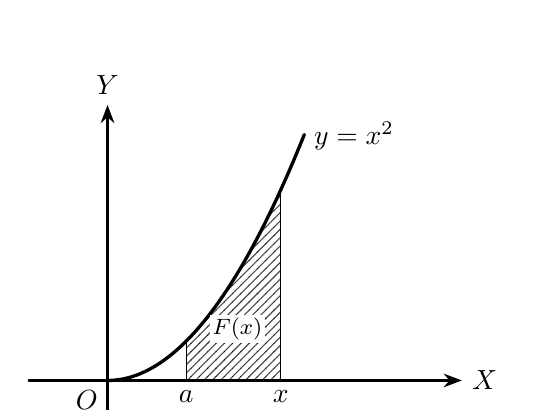
\begin{tikzpicture}[>=Stealth, scale=1.0, line cap=round, line join=round]
  \draw[->, thick] (-1.0, 0) -- (4.5, 0) node[right] {$X$};
  \draw[->, thick] (0, -0.5) -- (0, 3.5) node[above] {$Y$};
  \node[below left] at (0, 0) {$O$};

  \draw[line width=1.2pt, domain=0:2.5, samples=50] plot (\x, {0.5*\x*\x});
  \node[right] at (2.5, 3.1) {$y=x^2$};

  % 斜線面積 [a, x]
  \fill[pattern=north east lines, opacity=0.7] (1.0, 0) -- plot[domain=1.0:2.2] (\x, {0.5*\x*\x}) -- (2.2, 0) -- cycle;
  \draw (1.0, 0) node[below] {$a$} -- (1.0, 0.5);
  \draw (2.2, 0) node[below] {$x$} -- (2.2, 2.42);
  \node[fill=white, inner sep=1pt, font=\footnotesize] at (1.65, 0.65) {$F(x)$};
\end{tikzpicture}
\caption{圖 6-2\quad 面積函數 $F(x)$ 之幾何定義}
\label{fig:b6s-app4-area-func}
\end{figure}

如果固定 $a$，令 $x$ 變動，則 $F(x)$ 是一個定義在 $[a, \infty)$ 上的函數。由導函數的公式得
\[ F'(x) = x^2 \]
如令 $y=F'(x)$，則上式就是原來曲線的方程式：這就表示曲線在 $x$ 軸之上自 $a$ 到 $x$ 的面積函數 $F(x)$ 的導函數等於原來所給的函數。

在一般情形，我們也有這種面積與導數的關係，敘述如下：

\begin{theorem}[微積分基本定理]\label{thm:b6s-app4-ftc}
設 $f(x)$ 是區間 $[a, b]$ 上的連續函數，$f(x)\ge 0$。令曲線 $y=f(x)$ 在 $[a, x], a\le x\le b$ 之上的面積為 $F(x)$，則
\begin{equation}
F'(x) = f(x) \tag{I} \label{eq:b6s-app4-ftc-1}
\end{equation}
而且曲線 $y=f(x)$ 在區間 $[c, d], a\le c<d\le b$ 之上的面積等於 $F(d)-F(c)$。
\end{theorem}

\begin{figure}[H]
\centering
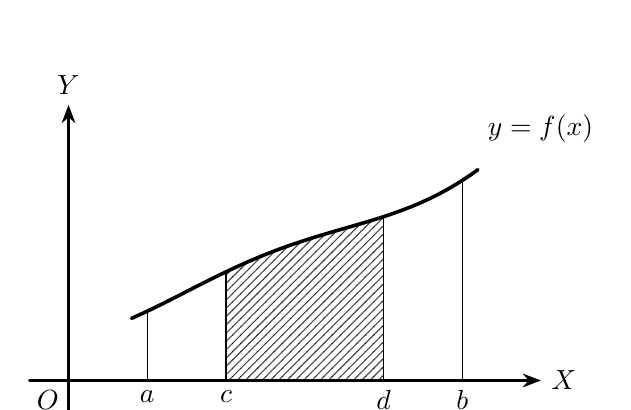
\begin{tikzpicture}[>=Stealth, scale=1.0, line cap=round, line join=round]
  \draw[->, thick] (-0.5, 0) -- (6.0, 0) node[right] {$X$};
  \draw[->, thick] (0, -0.5) -- (0, 3.5) node[above] {$Y$};
  \node[below left] at (0, 0) {$O$};

  \draw[line width=1.3pt, domain=0.8:5.2, samples=50] plot (\x, {0.8 + 0.3*sin((\x-1)*60) + 0.08*\x*\x});
  \node[right] at (5.2, 3.2) {$y=f(x)$};

  \fill[pattern=north east lines, opacity=0.7] (2.0, 0) -- plot[domain=2.0:4.0] (\x, {0.8 + 0.3*sin((\x-1)*60) + 0.08*\x*\x}) -- (4.0, 0) -- cycle;
  \draw (1.0, 0) node[below] {$a$} -- (1.0, 0.88);
  \draw (2.0, 0) node[below] {$c$} -- (2.0, 1.38);
  \draw (4.0, 0) node[below] {$d$} -- (4.0, 2.08);
  \draw (5.0, 0) node[below] {$b$} -- (5.0, 2.54);
\end{tikzpicture}
\caption{圖 6-3\quad 連續函數曲線下面積之微積分基本定理}
\label{fig:b6s-app4-ftc-geom}
\end{figure}

在定理中，我們假定 $f(x)\ge 0$，只是為了方便，容易看出直觀的意義。又因為滿足 \eqref{eq:b6s-app4-ftc-1} 式的任意兩個函數至多相差一個常數（可由均值定理導出），所以在求面積時只要找到其中任意一個就可以了。

\begin{example}\label{ex:b6s-app4-27}
求 $y=x$ 在 $[1, 4]$ 之上的面積。
\end{example}

\paragraph{【解】}
令 $F(x)=\dfrac{x^2}{2}$，則 $F'(x)=x$。所以由上面的定理得到所求面積為
\[ F(4)-F(1) = \dfrac{4^2}{2} - \dfrac{1^2}{2} = \dfrac{15}{2} \text{。}\hfill\# \]

\begin{example}\label{ex:b6s-app4-28}
求 $y=x^3$ 在 $[2, 5]$ 之上的面積。
\end{example}

\paragraph{【解】}
令 $F(x)=\dfrac{x^4}{4}$，則 $F'(x)=x^3$。所求面積為
\[ F(5)-F(2) = \dfrac{5^4}{4} - \dfrac{2^4}{4} = \dfrac{609}{4} \text{。}\hfill\# \]

\begin{example}\label{ex:b6s-app4-29}
求 $y=\sin x$ 在 $[0, \pi]$ 之上的面積。
\end{example}

\paragraph{【解】}
令 $F(x)=-\cos x$，則 $F'(x)=\sin x$。所求面積為
\[ F(\pi)-F(0) = -\cos\pi - (-\cos 0) = 1 - (-1) = 2 \text{。}\hfill\# \]

\begin{example}\label{ex:b6s-app4-30}
求 $y=e^x$ 在 $[a, b]$（$a, b$ 為任意實數，但 $a<b$）之上的面積。
\end{example}

\paragraph{【解】}
令 $F(x)=e^x$，則 $F'(x)=e^x$。故所求面積為 $e^b - e^a$。\hfill$\#$

\subsubsection*{習題 6}\label{sec:b6s-ex-app4-6}

\begin{enumerate}[label=\arabic*., leftmargin=2em]
  \item 求直線 $y=2x$ 在 $[1, 4]$ 之上的面積。
  \item 求直線 $y=3x+6$ 在 $[0, 3]$ 上的面積。
  \item 求拋物線 $y=x^2+1$ 在 $[0, 1]$ 上的面積。
  \item 求拋物線 $y=3x^2+2x+1$ 在 $[0, 2]$ 上的面積。
  \item 求曲線 $y=\cos\theta$ 在 $\left[0, \frac{\pi}{2}\right]$ 上的面積。
  \item 求曲線 $y=\dfrac{1}{x}$ 在 $[1, 5]$ 上的面積。
  \item 求 $y^2=x$ 與 $x-2y=4$ 所包圍區域的面積。
  \item 求 $xy=1$ 與 $x+y=4$ 所包圍區域的面積。
\end{enumerate}
\renewcommand{\thetheorem}{\arabic{theorem}}
\renewcommand{\thelemma}{\arabic{lemma}}


\end{document}
